%% LyX 2.1.3 created this file.  For more info, see http://www.lyx.org/.
%% Do not edit unless you really know what you are doing.
\documentclass[12pt,oneside,english,reqno]{amsbook}
\renewcommand{\familydefault}{\rmdefault}
\usepackage[T1]{fontenc}

\usepackage{geometry}
\geometry{verbose,tmargin=1in,bmargin=1in,lmargin=1in,rmargin=1in}
\usepackage{mathrsfs}
\usepackage{url}
\usepackage{amsbsy,latexsym,amsmath}
\usepackage{amsfonts}
\usepackage{amssymb}
\usepackage[mathscr]{eucal}
\usepackage{epsfig,graphics,graphicx}
\usepackage{color}
\usepackage{amsthm}
\usepackage{amstext}
\usepackage{stmaryrd}
\usepackage{graphicx}
\usepackage{setspace}
\doublespacing

\makeatletter

%%%%%%%%%%%%%%%%%%%%%%%%%%%%%% LyX specific LaTeX commands.
%% A simple dot to overcome graphicx limitations
\newcommand{\lyxdot}{.}
%%%%%%%
\newtheorem{lemma}{Lemma}

 \newcommand{\abs}[1]{\left|{#1}\right|}
 \newcommand{\av}[1]{\left\langle #1 \right\rangle}
 
  \newcommand{\br}[1]{\langle #1|}
  \newcommand{\ke}[1]{|#1\rangle}
  \newcommand{\bk}[2]{\langle #1|#2\rangle}
  \newcommand{\kb}[2]{\ke{#1}\br{#2}}
  \newcommand{\var}[2]{\langle #1,#2\rangle} 
  
  \newcommand{\al}[1]{^{(#1)}}
  \newcommand{\da}{^\dagger} 
  
  \newcommand{\pt}[1]{\left( #1 \right)}
  \newcommand{\pq}[1]{\left[ #1 \right]}
  \newcommand{\pg}[1]{\left\{ #1 \right\}} 
  
  \newcommand{\lpt}[1]{\left( #1 \right.}
  \newcommand{\lpq}[1]{\left[ #1 \right.]}
  \newcommand{\lpg}[1]{\left\{ #1 \right.}
  \newcommand{\rpt}[1]{\left. #1 \right)}
  \newcommand{\rpq}[1]{\left. #1 \right]}
  \newcommand{\rpg}[1]{\left. #1 \right\}} 


\newcommand{\td}[1]{\widetilde{#1}}

%%%%%%%%%%%%%%%%%%%%%%%%%%%%%% Textclass specific LaTeX commands.
\numberwithin{section}{chapter}
\numberwithin{equation}{section}
\numberwithin{figure}{section}

\makeatother

\usepackage{babel}

\begin{document}


\global\long\def\sandwich#1#2#3{ \left\langle #1\left|#2\right|#3\right\rangle }
\global\long\def\ket#1{\left|#1\right>}
\global\long\def\braket#1#2{\left\langle #1\mid#2\right\rangle }
\global\long\def\bra#1{\left\langle #1\right|}
\global\long\def\indep{\perp\!\!\!\perp}




 \thispagestyle{empty}\pagenumbering{gobble}

\vphantom{}

\textbf{\large{}Quantum State Discrimination and Quantum Cloning: }{\large \par}

\textbf{\large{}\hspace{2.7cm}Optimization and Implementation }{\large \par}

\vspace{1.2cm}


{\huge{}\hspace{5cm}\hspace{1cm}\hspace{1cm}}by

\vspace{0.7cm}


{\huge{}\hspace{5cm}\hspace{1.1cm}}Lazy bum

\vfill{}


\begin{singlespace}
A dissertation submitted to the Graduate Faculty in Physics in partial
fulfillment of the requirements for the degree of Doctor of Philosophy,
The City University of New York 
\end{singlespace}

\begin{center}
2015
\par\end{center}

\pagebreak{}

 \pagenumbering{roman}\setcounter{page}{2}\vphantom{}

\begin{singlespace}
\begin{center}
\vfill{}

\par\end{center}

%\begin{center}
%\includegraphics[width=2cm]{../ugur_dissertation_copy/img/creative_commons_logo_by}
%\par\end{center}

\begin{center}
2015\\
Undeserving lazy bum\\
Some rights reserved.\\
This work is licensed under a Creative Commons\\
Attribution 4.0 United States License.\\
\url{http://creativecommons.org/licenses/by/4.0/}
\par\end{center}
\end{singlespace}

\pagebreak{}

\vphantom{}

\vfill{}


\begin{center}
\begin{minipage}[c][1\totalheight][t]{1\columnwidth}%
\begin{singlespace}
\begin{center}
This manuscript has been read and accepted for the\\
Graduate Faculty in Physics in satisfaction of the \\
dissertation requirement for the degree of Doctor of Philosophy.
\par\end{center}\end{singlespace}
%
\end{minipage}
\par\end{center}

\vspace{3cm}


\begin{minipage}[t]{0.25\columnwidth}%
\begin{singlespace}
\rule[0.5ex]{1\columnwidth}{1pt}

Date\end{singlespace}
%
\end{minipage} \hfill{}%
\begin{minipage}[t]{0.6\columnwidth}%
\begin{singlespace}
\rule[0.5ex]{1\columnwidth}{1pt}

Prof. J�nos A. Bergou

Chair of Examining Committee\end{singlespace}
%
\end{minipage}

\vspace{2cm}


\begin{minipage}[t]{0.25\columnwidth}%
\begin{singlespace}
\rule[0.5ex]{1\columnwidth}{1pt}

Date\end{singlespace}
%
\end{minipage} \hfill{}%
\begin{minipage}[t]{0.6\columnwidth}%
\begin{singlespace}
\rule[0.5ex]{1\columnwidth}{1pt}

Prof. Igor L. Kuskovsky

Executive Officer\end{singlespace}
%
\end{minipage}

\vspace{1.5cm}


\begin{center}
\begin{minipage}[t]{0.8\columnwidth}%
\begin{singlespace}
Supervisory Committee:

\vspace{1cm}


Prof. Mark Hillery\hfill{}

\vspace{1cm}


Prof. Steven Greenbaum\hfill{} 

\vspace{1cm}


Prof. Ed Feldman\hfill{}

\vspace{1cm}


Prof. Neepa T. Maitra\hfill{}\end{singlespace}
%
\end{minipage}
\par\end{center}

\vspace{0.5cm}


\begin{center}
THE CITY UNIVERSITY OF NEW YORK
\par\end{center}

\pagebreak{}

{\huge{}\hspace{5cm}\hspace{1.2cm}}\textbf{\Large{}Abstract}{\Large \par}

\vspace{1.5cm}


\textbf{\large{}Quantum State Discrimination and Quantum Cloning: }{\large \par}

\textbf{\large{}\hspace{2.7cm}Optimization and Implementation }{\large \par}

\vspace{1.2cm}


{\huge{}\hspace{5cm}\hspace{1cm}\hspace{1cm}}by

\vspace{0.7cm}


{\huge{}\hspace{5cm}\hspace{1.1cm}}Lazy Bum

\vspace{1cm}


\textbf{Advisor:}\textbf{\small{} }Janos A. Bergou

\vspace{1cm}

This thesis reflects works previously published by the author and materials 
hitherto unpublished on the subject of quantum information theory.  Particularly,
results in optimal discrimination, cloning, and separation of quantum states, 
and their relationships, are discussed.  Via Neumark's theorem \cite{Neumark}, 
our description of these unitary processes can be implemented with linear optical devices. 



{\huge{}\hspace{1.0cm}}\textbf{\Large{}}{\Large \par}

\vspace{1.5cm}

\vspace{1.2cm}

\chapter*{Acknowledgements}


\vspace{0.7cm}



\vspace{1cm}


THANKS BRUVS, MUCH LOVE!



\tableofcontents{}

\listoffigures


 \pagenumbering{arabic}\pagebreak{}

%%%%%%%%%%%%%%%%%%%%%%%%%%%%%%%%%%%%%%%%%%%%%%%%
%%%%%%%%%%%%%%%%%%%%%%%%%%%%%%%%%%%%%%%%%%%%%%%%
\chapter{Introduction}


\section{Properties of Measurement Theory}



Classical bits versus quantum bits: instead of just a 0 or 1, quantum bits can maintain a superposition state

The probabalistic nature of detection: only orthogonal states can be discriminated perfectly


Quantum Computing

Quantum Communication
 factorization work of Peter Schor \cite{Shor1994} and quantum
key distribution protocols such as B92 \cite{Bennett1992}. 

%%%%%%%%%%%%%%%%%%%%%%%%%%%%%%%%%%%%%%%%%%%%%%%%
%%%%%%%%%%%%%%%%%%%%%%%%%%%%%%%%%%%%%%%%%%%%%%%%
\section{State Representation and Measurements }

We begin by describing pure quantum states $\psi$ as vectors in a Hilbert space and an ensemble of states as
 $\rho  = \sum_i \eta_i \kb{\psi_ i}{\psi_i}$ where $\sum \eta_i = 1$. The evolution of this ensemble is the 
Schrodinger equation as
\[i \hbar \frac{\partial\rho}{\partial t} =  [H,\rho].\]
Solving this for time-independent evolution we get
\[\rho(t) = U(t) \rho(0) U(t)^\dagger.\]
and where the unitary matrix U obeys $UU^\dagger = I$.
There are several ways to view this formula. The first is by decomposing the unitary into a set of Kraus operators $A_i$
such that $U(\ke {\psi_A} \otimes \ke {\phi_B}) = \sum_i A_i \ke {\psi_A} \otimes \ke {i_B}$ and $\sum A_i A_i^\dagger = I$.
 The alternative effects of the evolution, for example a particle striking 
one detector as opposed to another, are described by the different operators $A_i$.  Blah blah measurement operators $\Pi_i$.

The other is due to Neumark \cite{Neumark1}. A unitary acts on a pure state $\psi$ to make state $\phi$, as in $U\ke \psi = \phi$.

Before we describe such processes particularly let us describe the mathematics of these structures.  The ensemble 
previously described can be describes as a density matrix.  This is a generalized state that is a statistical collection 
of pure states defined by four properties:

\begin{enumerate}
\item $\rho  = \sum_i \eta_i \kb{\psi_ i}{\psi_i}$ where $\sum \eta_i = 1$,
\item It is Hermitian ,
\item $Tr \rho = 1$,
\item $\br {\phi_i} \rho \ke {\phi_i} \geq 0$.
\end{enumerate}

The measurements $\Pi_i$ are a decomposition of the identity in terms of positive semi-definite matrices. 
A measurement can be either a projector onto an eigenvector of the Hilbert space or a generalized measurement.  In the latter case it must fulfill only 2 properties:

\begin{enumerate}
\item $\sum \Pi_i = 1$
\item They are Hermitian.  This corresponds to real eigenvalues (measurement outcomes).
\end{enumerate}

Since non-orthogonal states cannot be discriminated perfectly, we can speak of the probability of a given outcome:
	$\av {\Pi_i} = \sum_j \eta_j \br {\psi_j} \Pi_i \ke {\psi_j} = Tr(\Pi_i \rho)$


The generalization of the postulates of quantum mechanics in terms
of the POVM can be expressed as:
\begin{enumerate}
\item The decomposition of the identity in terms of positive operators,
$\Pi_{j}\geq0$, $\sum_{j}\Pi_{j}=I$ is called a POVM.
\item The elements of the POVM can be expressed in terms of the detection
operators $\Pi_{j}=A_{j}^{\dagger}A_{j}$ where the operators satisfy
the requirements $\sum_{j}A_{j}^{\dagger}A_{j}=I$ but they need not
be Hermitian.
\item A detection yields an element on POVM.
\item The state of the system collapses onto: $\ket{\phi_{j}}=\frac{A_{j}\ket{\psi}}{\sqrt{\sandwich{\psi}{A_{j}^{\dagger}A_{j}}{\psi}}}$
if the system was initially in a pure state, $\rho_{j}=\frac{A_{j}^{\dagger}\rho A_{j}}{Tr(A_{j}\rho A_{j}^{\dagger})}=\frac{A_{j}^{\dagger}\rho A_{j}}{Tr(A_{j}^{\dagger}A_{j}\rho)}=\frac{A_{j}^{\dagger}\rho A_{j}}{Tr(\Pi_{j}\rho)}$
if the system was initially in a mixed state. 
\item The probability of obtaining $\rho_{j}$ is $p_{j}=Tr(A_{j}\rho_{j}A_{j}^{\dagger})=Tr(A_{j}^{\dagger}A_{j}\rho_{j})=Tr(\Pi_{j}\rho_{j})$.
\item If a measurement is performed but the result is not recorded the post-measurement
state collapses onto: $\tilde{\rho}=\sum_{j}p_{j}\rho_{j}=\sum_{j}A_{j}\rho A_{j}^{\dagger}$.
\end{enumerate}
\subsection{Standard Quantum Measurements}

We start with the postulates of standard or projective quantum measurements
introduced by von Neumann \cite{Neumann1955} analyzing a model for
the coupling of the system with the meter or ancilla and generalizing
the predictions of the model. 

The postulates are:
\begin{enumerate}
\item Observables in quantum mechanics have a Hermintian operator $\chi$
which has a spectral representation $\chi=\sum_{j}^{N}\lambda_{j}\ket j\bra j$,
where the eigenvalues are real and assuming non-degeneracy for simplicity.
The eigenvectors $\left\{ \ket j\right\} $ form a complete orthonormal
basis set.
\item The Hilbert space is spanned by the projectors $P_{j}=\ket j\bra j$,
such that $\sum_{j}P_{j}=1.$ 
\item The eigenvalues of the projectors are $0$ or $1$ due to the orthogonality
of the states $P_{i}P_{j}=P_{i}\delta_{ij}$.
\item Any measurement of the $\chi$ will yield one of the eigenvalues $\lambda_{j}$.
\item If $\lambda_{j}$ is obtained in a measurements, the state of the
system collapses onto: $\ket{\phi_{j}}=\frac{P_{j}\ket{\psi}}{\sqrt{\sandwich{\psi}{P_{j}}{\psi}}}$
if the system was initially in a pure state, $\rho_{j}=\frac{P_{j}\rho P_{j}}{Tr(P_{j}\rho)}$
if the system was initially in a mixed state. 
\item The probability of obtaining $\ket{\phi_{j}}$ is $p_{j}=\left|\left|P_{j}\psi\right|\right|^{2}=\sandwich{\psi}{P_{j}^{2}}{\psi}=\sandwich{\psi}{P_{j}}{\psi}$.
The probability of obtaining $\rho_{j}$ is $p_{j}=Tr(P_{j}\rho P_{j})=Tr(P_{j}^{2}\rho)=Tr(P_{j}\rho)$. 
\item If a measurement is performed but the result is not recorded the post-measurement
state collapses onto: $\rho=\sum_{j}P_{j}\ket{\psi}\bra{\psi}P_{j}$
if the system was initially in a pure state, $\tilde{\rho}=\sum_{j}p_{j}\rho_{j}=\sum_{j}P_{j}\rho P_{j}$
if the system was initially in a mixed state.
\end{enumerate}



%%%%%%%%%%%%%%%%%%%%%%%%%%%%%%%%%%%%%%%%%%%%%%%%
%%%%%%%%%%%%%%%%%%%%%%%%%%%%%%%%%%%%%%%%%%%%%%%%%%%%%%%%%%%%%%%%%%%%%%%%%%%%%%%%%%%%%%%%%%%%%%%%
%%%%%%%%%%%%%%%%%%%%%%%%%%%%%%%%%%%%%%%%%%%%%%%%
\chapter{Discrimination of Pure States}
Consider the problem of discriminating between two states $\ke \psi_1$ and $\ke \psi_2$.  If we could always perform this perfectly
then we should be able to write a unitary U such that 
\begin{eqnarray}
U\ke {\psi_1}= \ke 1,\\
U\ke {\psi_2} = \ke 2,
\end{eqnarray}
where the states $\ke 1$ and $\ke 2$ are orthogonal in the basis of the input states, and each result is associated with the respective input.  However
since the unitary is inner-product preserving, taking the product of the first with the second's adjoint shows
this unitary and hence such a measurement are impossible unless the input states are orthogonal:
\[\br {\psi_2} U^\dagger U \ke {\psi_1} = \bk {\psi_2}{\psi_1} = \bk 1 2 = 0.  \]
We can make a similar demonstration
using the operator method.  If 
\begin{equation}
\Pi_1 \ke {\psi_2} = 0 \\
\Pi_2 \ke {\psi_1} = 0
\end{equation} 
then using $\Pi_1 + \Pi_2 = I$ and inner product of these equations, we get the same result:
\[0= \br{\psi_2} \Pi_1 + \Pi_2 \ke {\psi_1} = \bk{\psi_1}{\psi_2} \]

 Since the two constraints of measurement,
orthogonality of the measurement vectors and their spanning the space, proved contradictory, we must give up one of these two
functions in order to perform a physical measurement.
 Hence we must choose a unitary that performs this task optimally according to some figure of merit, typically a probability measure.  For all future discussion
we assume that the input states $\psi_1$ and $\psi_2$ are provided one at a time, 
and with known probabilities $\eta_1$ and $\eta_2$ respectively, such that $\eta_1 + \eta_2 = 1$.  



%%%%%%%%%%%%%%%%%%%%%%%%%%%%%%%%%%%%%%%%%%%%%%%%
%%%%%%%%%%%%%%%%%%%%%%%%%%%%%%%%%%%%%%%%%%%%%%%%
\section{Minimum Error Discrimination}
Historically, the first solution to this problem is due to Helstrom \cite{Helstrom1969}.  
Now known as the Minimum Error (ME) strategy, the figure of merit is the average rate
of mistakingly identifying one state for the other.  Using the density matrix and trace notation,
this average probability of error can be written as
\[P_e = \eta_1 tr[\rho_1 \Pi_2] + \eta_2 tr[\rho_2 \Pi_1],\]
where we associate the outcome $\Pi_i$ with state $\psi_i$.
Analagously, the average probability of success is simply 
\[P_s = \eta_1 tr[\rho_1 \Pi_1] + \eta_2 tr[\rho_2 \Pi_2],\]
Because we want a result every time a state is sent to us the
operators $\Pi_i$ must span the space, so $\Pi_1 + \Pi_2 = I$ which implies $P_e + P_s =1$.  The minimum error is attained at the Helstrom bound:
\begin{equation}
P_{E}=\frac{1}{2}[1-\sqrt{1-4\eta_{1}\eta_{2}|\langle\psi_{1}|\psi_{2}\rangle|^{2}}].
\end{equation}
The detectors and states can are graphically represented in Fig. 1 for the case when the given states are qubits and occur with equal likelihood.

\begin{figure}
\begin{centering}
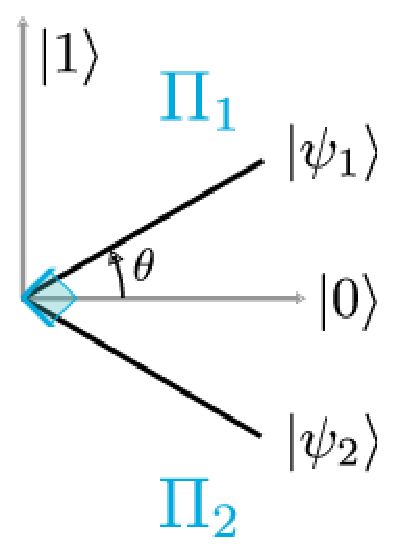
\includegraphics[width=8.5cm,height=8.5cm]{ME}\protect\caption[\hspace{1cm}Min Error]{ The states $\psi_i$ and projectors $\Pi_i = \kb {\phi_i}{\phi_i}$ which minimizes the error rate for detection.
along the states $\left\{ \protect\ket{\psi_{1}},\protect\ket{\psi_{2}}\right\} $
for $\eta_{1}=\eta_{2}=\frac{1}{2}$. }

\par\end{centering}

\label{POVM_ME} 
\end{figure}

We provide a derivation of this result to demonstrate the Neumark formalism.
Since both $\psi_1$ and $\psi_2$ can now evolve to either $0$ or $1$, we must write the unitary equations as
\begin{eqnarray}
U \ke{\psi_1} = \sqrt{p_1} \ke 1 + \sqrt{r_1} \ke 2\\
U \ke{\psi_2} = \sqrt{p_2} \ke 2 + \sqrt{r_2} \ke 1,\label{eq:ME neumark}
\end{eqnarray}
where $p_i$ and $r_i$ are the individual success and error probabilities of the measurement.  Taking the inner product of these 
two equations with themselves we find $p_i + r_i = 1$, and taking the inner product with each other we get the overlap constraint

\begin{equation}
s = \bk{\psi_1}{\psi_2} = \sqrt{p_1 r_2} + \sqrt{ p_2 r_1}, \label{eq:ME constraint}
\end{equation}

We wish to minimize the average error rate

\begin{equation}
P_{E}=\eta_{1}r_{1}+\eta_{2}r_{2},\label{eq:ME}
\end{equation}

subject to the constraint in (\ref{eq:ME constraint}).  We solve this two variable problem using the method of Lagrange multipliers.  
For details on this method see Appendix 2.  The constrained error equation can be written as

\begin{equation}
F(r_1,r_2,\lambda)=\eta_{1}r_{1}+\eta_{2}r_{2}+\lambda\left[s-\sqrt{(1-r_{1})r_{2}}-\sqrt{(1-r_{2})r_{1}}\right].
\end{equation}

Our extrema will be found when all partial derivatives of this equation are zero, therefore

\[
\frac{\partial F_{E}}{\partial r_{1}}=\eta_{1}+\frac{1}{2}\left[\sqrt{\frac{r_{2}}{1-r_{1}}}-\sqrt{\frac{1-r_{2}}{r_{1}}}\right]=0,
\]
and

\[
\frac{\partial F_{E}}{\partial r_{2}}=\eta_{2}+\frac{1}{2}\left[-\sqrt{\frac{r_{1}}{1-r_{2}}}+\sqrt{\frac{1-r_{1}}{r_{2}}}\right]=0.
\]

We notice that these two equations may be re-arranged such that the left hand side is dependent on a single variable:


\begin{equation}
\frac{2\eta_{1}}{\lambda}\sqrt{r_{1}(1-r_{1})}=\sqrt{r_{1}r_{2}}-\sqrt{(1-r_{1})(1-r_{2})},\label{eq:r12}
\end{equation}


\begin{equation}
\frac{2\eta_{2}}{\lambda}\sqrt{r_{2}(1-r_{2})}=\sqrt{r_{1}r_{2}}-\sqrt{(1-r_{1})(1-r_{2})}.\label{eq:r1r2}
\end{equation}


The right hand sides of Eq.(\ref{eq:r12}) and (\ref{eq:r1r2}) can
be set to a constant $\frac{2\eta_{i}}{\lambda}\sqrt{r_{i}(1-r_{i})}\equiv C$,
which can later be determined from the unitarity constraint \ref{eq:ME constraint}, 

\begin{eqnarray}
r_{i} & = & \frac{1}{2}\left(1\pm\sqrt{1-\frac{\lambda^{2}C^{2}}{\eta_{i}^{2}}}\right)=\frac{1}{2}\left(1-\sqrt{1-\frac{\delta^{2}}{\eta_{i}^{2}}}\right),\label{eq:r_i-1}\\
r_{i} & = & \frac{1}{2}\left[1-A_{i}\right],
\end{eqnarray}


where $A_{i}\equiv\sqrt{1-\frac{\delta^{2}}{\eta_{i}^{2}}}$ and $\delta^{2}\equiv\lambda^{2}C^{2}$.
The smaller $r_{i}$ is picked (lower sign in \ref{eq:r_i-1} ) as
this represents error rate, which is to be minimized. Now replace
$r_{i}$ into the constraint (\ref{eq:ME constraint}) and solve for
$\delta$:

\begin{eqnarray*}
s & = & \sqrt{(1-r_{1})r_{2}}+\sqrt{(1-r_{2})r_{1}},\\
2s & = & \sqrt{(1+A_{1})(1-A_{2})}+\sqrt{(1-A_{1})(1+A_{2})},\\
2s^{2} & = & 1-A_{1}A_{2}+\sqrt{(1-A_{1}^{2})(1-A_{2}^{2})},\\
2s^{2} & = & 1-A_{1}A_{2}+\frac{\delta^{2}}{\eta_{1}\eta_{2}},\\
(2s^{2}-1 & -\frac{\delta^{2}}{\eta_{1}\eta_{2}})^{2}= & 1-\frac{\delta^{2}}{\eta_{1}^{2}}-\frac{\delta^{2}}{\eta_{2}^{2}}+\frac{\delta^{4}}{\eta_{1}^{2}\eta_{2}^{2}}.
\end{eqnarray*}


After some tedious but trivial algebra:

\begin{equation}
\delta^{2}=\frac{4s^{2}(1-s^{2})\eta_{1}^{2}\eta_{2}^{2}}{1-4\eta_{1}\eta_{2}s^{2}}.\label{eq:delta}
\end{equation}


Now substitute the value of $\delta$ from (\ref{eq:delta}) into
(\ref{eq:r_i-1}) to get the explicit form of the individual error
rates,

\begin{equation}
r_{i}=\frac{1}{2}\left[1-\frac{1-2\eta_{i}s^{2}}{\sqrt{1-4\eta_{1}\eta_{2}s^{2}}}\right]
\end{equation}


Inserting $r_{1}$ and $r_{2}$ into (\ref{eq:P_E}) Helstrom bound
is retrieved \cite{Helstrom1969}

\begin{eqnarray}
P_{E} & = & \frac{1}{2}\left[1-\frac{\eta_{1}-2\eta_{1}\eta_{2}s^{2}}{\sqrt{1-4\eta_{1}\eta_{2}s^{2}}}-\frac{\eta_{2}-2\eta_{1}\eta_{2}s^{2}}{\sqrt{1-4\eta_{1}\eta_{2}s^{2}}}\right],\nonumber \\
P_{E} & = & \frac{1}{2}\left[1-\sqrt{1-4\eta_{1}\eta_{2}s^{2}}\right].
\end{eqnarray}

%%%%%%%%%%%%%%%%%%%%%%%%%%%%%%%%%%%%%%%%%%%%%%%%
%%%%%%%%%%%%%%%%%%%%%%%%%%%%%%%%%%%%%%%%%%%%%%%%
\section{Unambiguous Discrimination}

It was noticed by *UD CITations** that we may completely eliminate error from the measurement results
by giving up the constraint that our two measurement operators span the whole space, $\Pi_1 + \Pi_2 = I$.  This creates an additional result which 
is not associated with the state being either $\psi_1$ or $\psi_2$ .  It is called the inconclusive or failure outcome $\Pi_0$,
and the new decomposition of the identity reads $\Pi_0+ \Pi_1 + \Pi_2 = I$.  


\begin{eqnarray}
\Pi_{1} & = & \frac{p_{1}}{|\langle\psi_{1}|\psi_{2}^{\perp}\rangle|^{2}}|\psi_{2}^{\perp}\rangle\langle\psi_{2}^{\perp}|,\nonumber \\
\Pi_{2} & = & \frac{p_{2}}{|\langle\psi_{2}|\psi_{1}^{\perp}\rangle|^{2}}|\psi_{1}^{\perp}\rangle\langle\psi_{1}^{\perp}|.\label{eq:Pi1Pi2}
\end{eqnarray}


To determine the failure operator, insert (\ref{eq:Pi1Pi2}) into
(\ref{eq:3povms}): 

\begin{equation}
\Pi_{0}=I-\Pi_{1}-\Pi_{2}=I-\frac{p_{1}}{|\langle\psi_{1}|\psi_{2}^{\perp}\rangle|^{2}}|\psi_{2}^{\perp}\rangle\langle\psi_{2}^{\perp}|-\frac{p_{2}}{|\langle\psi_{2}|\psi_{1}^{\perp}\rangle|^{2}}|\psi_{1}^{\perp}\rangle\langle\psi_{1}^{\perp}|.
\end{equation}

The eigenvalues of $\Pi_{0}$ must be non-negative, giving us the inequality constraint between the individual failure rates as

\begin{equation}
q_{1}q_{2}\geq|\langle\psi_{1}|\psi_{2}\rangle|^{2}.\label{eq:qConstraint}
\end{equation}
 where we used $q_{i}=1-p_{i}.$

Now our value of merit will be the average failure rate $Q = \eta_1 q_1 + \eta_2 q_2$.  Since there is no error the success and failure
add to one: $P_s + Q = 1$.  Hence we wish to minimize the failure rate by taking the equality in Eq. (\ref{eq:qConstraint}), giving us the minimum
failure rate at
\begin{equation}
Q \equiv Q_0 = 2 \sqrt{\eta_1 \eta_2}|\langle\psi_{1}|\psi_{2}\rangle|. \label{Q0}
\end{equation}

This solution is valid for $q_{i}\leq1.$  Outside of this bound we ignore the state with the high rate of failure by removing that detector and
reducing our measurement strategy back to projective measurements.  We project onto the more likely state.  Therefore the total UD solution is
\begin{equation}
Q_{{\rm c}}=\left\{ \begin{array}{l}
\eta_{1}+\eta_{2}\cos^{2}\theta,\mbox{if \ensuremath{{\displaystyle \eta_{1}<\frac{\cos^{2}\theta}{1+\cos^{2}\theta}\equiv\eta_{1}^{(l)}}},}\\[0.7em]
\eta_{2}+\eta_{1}\cos^{2}\theta,\mbox{if \ensuremath{\eta_{1}>{\displaystyle \frac{1}{1+\cos^{2}\theta}\equiv\eta_{1}^{(r)}}},}\\[0.7em]
2\sqrt{\eta_{1}\eta_{2}}\cos\theta\equiv Q_{0},\mbox{if \ensuremath{\eta_{1}^{(l)}\le\eta_{1}\le\eta_{1}^{(r)}}}\ ,
\end{array}\right.\label{Qmax}
\end{equation}



%%%%%%%%%%%%%%%%%%%%%%%%%%%%%%%%%%%%%%%%%%%%%%%%
%%%%%%%%%%%%%%%%%%%%%%%%%%%%%%%%%%%%%%%%%%%%%%%%
\section{Interpolative Discrimination}
\subsection{Operator Transformation}


%[floatfix]
\begin{figure}[ht!]
\centering{ 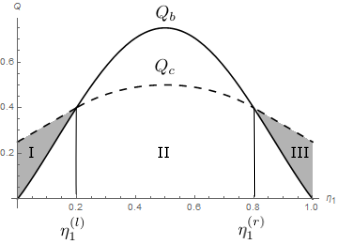
\includegraphics[height=4.5cm]{Fig1.png}}
\protect\caption[\hspace{1cm}$Q_{{\rm c}}$ and $Q_{{\rm b}}$ vs.~$\eta_{1}$]{ $Q_{{\rm c}}$ (dashed line, Eq. (\ref{Qmax})) and $Q_{{\rm b}}$
(solid line, Eq. (\ref{Qb})) vs.~$\eta_{1}$ for $\theta=\pi/3$.
Measurements can be optimized in the area under the dashed line, $Q_{c}$.
Measurements in the area above $Q_{c}$ are suboptimal. In the shaded
areas between $Q_{c}$ and $Q_{b}$ (regions I, left, and III, right)
the optimal FRIO measurement is a projective measurement, in the unshaded
area below $Q_{c}$ (region II) the optimal measurement is a POVM.}
\label{Fig1} 
\end{figure}


We review the original problem in a single two-dimensional Hilbert space, and the solution that  involves a transformation that eliminates the failure operator from the discrimination problem.  We are given two pure states $\rho_1= \ke \psi_1 \br {\psi_1}$ and $\rho_2 = \ke \psi_2 \br{\psi_2}$ with a-priori probabilities $\eta_1$ and $\eta_2$ respectively.  These two probabilities add to one:  $\eta_1 +\eta_2 = 1$. We wish to optimize the success rate  $P_s = \eta_1tr[\Pi_1 \rho_1] + \eta_2 tr[\Pi_2 \rho_2]$ for a fixed failure rate $Q = tr[\Pi_0(\eta_1 \rho_1 + \eta_2 \rho_2)]$ where the measurement operators are the $\Pi_i$ that span the Hilbert space: $\Pi_1 + \Pi_2 + \Pi_0 = I$.  The transformation we implement is
 \begin{equation}
\Omega ^{-1/2}[\Pi_1 + \Pi_2] \Omega^{-1/2} = I,
\end{equation}
where $\Omega = I - \Pi_0$.

Calling the transformed operators $\widetilde \Pi_i$ for $i= 1,2$, we can find the corresponding transformed density matrices $\widetilde \rho_i$ and a-priori probabilities $
\widetilde \eta_i$ to make this a new ME problem that can be readily solved. The minimized error probability as a function of the failure rate is
\begin{equation} P_e = \frac{1}{2} (1 - Q -\sqrt{(1-Q)^2 - (Q-Q_0)^2})\end{equation}
for $Q \leq Q_0 = 2 \sqrt{\eta_1\eta_2} \cos \theta$ where $Q_0$ is the maximum failure rate allowed in the optimization scheme and it corresponds to the best measurement in the UD case.  We will provide an in-depth description of this solution as it pertains to our problem in the next section.



%%%%%%%%%%%%%%%%%%%%%%%%%%%%%%%%%%%%%%%%%%%%%%%%
%%%%%%%%%%%%%%%%%%%%%%%%%%%%%%%%%%%%%%%%%%%%%%%%

\subsection{Neumark Solution of Interpolation}

Since our measurement results must now include the three degrees of freedom from the successful measurements and failure result, in addition to the two degrees of freedom
provided us by the pure states, we require an extra ancillary degree of freedom.  This we add by extending our Hilbert space with a direct sum extension.

\begin{eqnarray}
U \ke {\psi_1}= \sqrt{p_1} \ke 1 + \sqrt{r_1} \ke 2 + \sqrt{q_1} \ke 0 \\
U |\psi_2 \rangle = \sqrt{r_2} \ke 1 + \sqrt{p_2} \ke 2 + \sqrt{q_2} \ke 0 
\end{eqnarray}

Here $p_i$ is the probability that the state i is correctly identified when it is sent into the measurment apparatus, $r_i$ the error rate (mistaking one state for the other) and $q_i$ the failure rate, or not getting a conclusive measurement result.  By sandwiching the preceding equations with their adjoints we confirm that $q_i + r_i+p_i = 1$, the sum of various probabilities is one.

\subsubsection{Equal Weights Solution}

The solution when $\eta_1 = \eta_2=\frac{1}{2}$ is very simple and neat.  Here we have $p_1 = p_2$, $q_1 =q_2$ and $r_1 = r_2$.  Hence $Q = \eta_1 q_1 + \eta_2 q_2 = q_1$

The overlap between the two states $\bk {\psi_2}{\psi_1} = s$ can be also found  by finding the adjoint of one of the Unitary expressions and sandwiching it with the other expression, and since $U U^\dagger = 1$   we find 

\[s = 2 \sqrt{pr} + Q = s \sqrt{p(1-p-q)} + Q\]
Solving for p by squaring we find
\[ (s- Q)^2 = 4p(1-p-q)\] so
\[p^2 -p(1-Q) + (s-Q)^2/4 = 0\] and the positive root gives us the answer as
\[p = \frac{1}{2}[1-Q - \sqrt{(1-Q)^2 -(s-Q)^2}]\]


%%%%%%%%%%%%%%%%%%%%%%%%%%%%%%%%%%%%%%%%%%%%%%%%%%%%%%%%%%%%%%%%%% %%%%%%%%%%%%%%%%%%%%%%%%%%%%%%%%%%%%%%%%%%%%%%%%%%%%%%%%%%%%%%%%%%%%%%%%%%%%%%%%%%%%%%%%%%%%%%%%%%%%%%%%%%%%%%%%%%%%%%%%%%%% 

\subsection{Full Solution}
The total probability of success, error and failure we denote as $P_s = \eta_1 p_1 + \eta_2 p_2$ and $P_r = \eta_1 r_1 + \eta_2 r_2$ and $Q = \eta_1 q_1 + \eta_2 q_2$ respectively.


Taking the inner product

\[s = \langle\psi_1|\psi_2\rangle\ = \sqrt{p_1 r_2} + \sqrt{p_2 r_1} + \sqrt{q_1 q_2}\]

\[= \sqrt{(1-r_1 -q_1 )r_2} + \sqrt{(1-r_2 -q_2 )r_1} + \sqrt{q_1 q_2}\]

This is our overlap constraint.

We now use the Lagrange multiplier method to minimize $P_e$ subject to the overlap constraint.

\[F_e = \eta_1 r_1 + \eta_2 r_2 + \lambda (s - Overlap Constraint )\]

Step one: \[dF/dr_i = 0\]	

 Solve for $r_i (\lambda)$
	
Step two: substitute $s = \sqrt{p_1 r_2} + \sqrt{p_2 r_1} + \sqrt{q_1 q_2}$	
 into $r_i (\lambda)$ and solve for $\lambda$, then plug $\lambda$ into $r_i (\lambda)$.
The details of this calculation are included in Appnedix A.

A lot of algebra gives us the individual error rates as:


\[r_1=\frac{1}{2}[\alpha_1-\frac{[2\eta_2\omega-\alpha_1(1-Q)]}{\sqrt{(1-Q)^2-4\omega\eta_1\eta_2}}]\]


and

\[r_2=\frac{1}{2}[\alpha_2-\frac{[2\eta_1\omega-\alpha_2(1-Q)]}{\sqrt{(1-Q)^2-4\omega\eta_1\eta_2}}]\]


where $\alpha_i \equiv 1-q_i $ and  $\omega\equiv(s -\sqrt{q_1 q_2})^2$

These are not the final result because they were optimized individually. Let us now put these into the expression of minimum error and do a final optimization. First

\[P_E =\eta_1 r_1+\eta_2 r_2\]

\[=\frac{1}{2}[(1-Q)-\sqrt{(1-Q)^2-4\eta_1\eta_2(s-\sqrt{q_1q_2})^2}]\]

We can further minimize this expression since total $Q$ is fixed but we can choose how much of it to place on $q_1$ and $q_2$

To minimize the above expression we can maximize the term under the square root

\[(1-Q)^2-4\eta_1\eta_2(s-\sqrt{q_1q_2})^2\]
\[ = (1-Q)^2-4\eta_1\eta_2(s-\sqrt{\frac{q_1(Q-\eta_1 q_1)}{\eta_2}})^2\]

Since the only part of this expression that is dependent on the variables $q_i$ is the inner square root, we can find an extremum of this part. A simple partial derivative with respect to $q_1$ tells us the optimality condition is $Q = 2 \eta_1 q_1$ or equivalently $\eta_1 q_1 = \eta_2 q_2$

This simplifies our solution to be 


\[P_E=\frac{1}{2}[(1-Q)-\sqrt{(1-Q)^2-(Q-Q_0)^2}]\]


%%%%%%%%%%%%%%%%%%%%%%%%%%%%%%%%%%%%%%%%%%%%%%%%
%%%%%%%%%%%%%%%%%%%%%%%%%%%%%%%%%%%%%%%%%%%%%%%%
\subsection{Transformation of the problem into the Helstrom form}


%%%%%%%%%%%%%%%%%%%%%%%%%%%%%%%%%%%%%%%%%%%%%%%%
%%%%%%%%%%%%%%%%%%%%%%%%%%%%%%%%%%%%%%%%%%%%%%%%
\subsection{Lagrange Multipliers Method}

%%%%%%%%%%%%%%%%%%%%%%%%%%%%%%%%%%%%%%%%%%%%%%%%
%%%%%%%%%%%%%%%%%%%%%%%%%%%%%%%%%%%%%%%%%%%%%%%%
%%%%%%%%%%%%%%%%%%%%%%%%%%%%%%%%%%%%%%%%%%%%%%%%
%%%%%%%%%%%%%%%%%%%%%%%%%%%%%%%%%%%%%%%%%%%%%%%%
\chapter{Discrimination of Mixed States}


\section{Minimum Error Discrimination}


%%%%%%%%%%%%%%%%%%%%%%%%%%%%%%%%%%%%%%%%%%%%%%%%
%%%%%%%%%%%%%%%%%%%%%%%%%%%%%%%%%%%%%%%%%%%%%%%%
\section{Minimum Error: Two mixed states via POVM }

%%%%%%%%%%%%%%%%%%%%%%%%%%%%%%%%%%%%%%%%%%%%%%%%
%%%%%%%%%%%%%%%%%%%%%%%%%%%%%%%%%%%%%%%%%%%%%%%%
\section{Mixed States with Jordan Structure}
\subsection{Jordan Basis Structure}

In this section we discuss the interpolative discrimination of a class of mixed states with a Jordan structure.  As before, 
they are to be discriminated with a-priori probabilities $\eta_1 , \eta_2$ but now their density matricies are 
\begin{eqnarray}
\rho_1 = \sum_i r_i \vert r_i \rangle \langle r_i \vert, \\
\rho_2 = \sum_i s_i \vert s_i \rangle \langle s_i \vert, \\
 \langle r_i \vert s_j \rangle = \delta_{ij} \cos \theta_i.
\end{eqnarray}

 In each 2d subspace i there lie an $\vert r_i \rangle$ and  $\vert s_i \rangle$ with a-priori probabilities now
$\eta_{1,i} = \eta_1 r_i$ and $\eta_{2,i} = \eta_2 s_i$.  This structure can be physically interpreted as the transmission of two input states over several fiber optic cables. Each cable contains two degrees of freedom, that could be horizontal and vertical polarization.

The generalization to multiple subspaces is straightforward at first  so we begin with the two subspaces example.

Here our density matrices are in four dimensions that can be described as two tensor product spaces:
\begin{eqnarray}
 \rho_1 &=& r_1 \vert r_1 \rangle \langle r_1 \vert  + r_2 \vert r_2 \rangle \langle r_2 \vert \\
 \rho_2 &=& s_1 \vert s_1 \rangle \langle s_1 \vert  + s_2 \vert s_2 \rangle \langle s_2 \vert. \nonumber\end{eqnarray}
These mixed states are shown in Fig. 1.


Defining our measurement operators for the first subspace as
\begin{equation} \widetilde \Pi_{1,1} + \widetilde \Pi_{2,1} = I_1,\end{equation}
where $I_1$ is the identity matrix of the first subspace.  We define the failure rate for the first subspace as $Q_1 = \xi_1 \ke 0_{11} \br 0 $,which in terms of a measurement probability is also
\begin{equation} Q_1 = \xi_1 [ \eta_{1,1} \cos^2 \phi_1 + \eta_{2,1} \cos^2 (\theta_1 - \phi_1)],\end{equation}
where $\theta_1 $ is the overlap angle between the two states in subspace 1, and $\phi_1$ is the angle $\ke {r_1}$ makes with respect to $\vert 0 \rangle_1$.  The error rate in that subspace is
\begin{equation}P_{e,1} = \eta_{1,1} \langle r_1 \vert \Pi_2 \vert r_1 \rangle + \eta_{2,1} \langle s_1 \vert \Pi_1 \vert s_1 \rangle. \end{equation}
For our simplification trick to work we introduce the normalized state vector \begin{equation} \vert \widetilde{r_1} \rangle  = \frac{ \Omega^{1/2} \vert r_1 \rangle}{\sqrt{\langle r_1 \vert \Omega \vert r_1 \rangle}} \end{equation}
and normalized coefficients
\begin{equation} \widetilde{\eta_{1,1}} = \frac{\eta_{1,1} \langle r_1 \vert \Omega \vert r_1 \rangle}{\eta_{1,1} \langle r_1 \vert \Omega \vert r_1 \rangle + \eta_{2,1} \langle s_1 \vert \Omega \vert s_1 \rangle}\end{equation}
to get 
\[P_{e,1}= \]
\[ [\eta_{1.1} \langle r_1 \vert \Omega \vert r_1 \rangle + \eta_{2,1}\langle s_1 \vert \Omega \vert s_1 \rangle](\widetilde{\eta_{1,1}}\langle\widetilde{r_1} \vert \widetilde{\Pi_2} \vert \widetilde{r_1} \rangle + \widetilde{\eta_{2,1}} \langle \widetilde{s_1} \vert \widetilde{\Pi_1} \vert \widetilde{s_1}\rangle ).\]

We notice that the expression in the ( ) with all tildes contains a pure state minimum error problem, while with the notation $ \eta_{1,1} +\eta_{2,1} = \omega_1$ the left hand set of [ ]  can be reworked into $\omega_1 - Q_1 $ to rewrite the error rate as
\[ P_{e,1}= \frac{1}{2} [\omega_1 - Q_1] (1- \sqrt{1 - 4 \widetilde{\eta_{1,1}} \widetilde{\eta_{2,1}} \vert \langle \widetilde{r_1} \vert \widetilde{s_1} \rangle \vert ^2 }). \]
If we substitute and simplify we find this equals to
\[=\frac{1}{2} ( \omega_1 - Q_1 - \sqrt{ ( \omega_1 - Q_1)^2 -(Q_{0,1} - Q_1 \sin 2 \phi )^2}),\]
where we used the notation $Q_{0,1} = 2 \sqrt{\eta_{1,1}\eta_{2,1}} \cos \theta_1$ and 
 $ \sin \phi = \frac{ \sqrt {\eta_{2,1}} \cos (\theta_1 - \phi_1)}{\sqrt{ \eta_{1,1} \cos^2 (\phi_1)+ \eta_{2,1} \cos^2 (\theta_1 - \phi_1)}}$.  Minimization of the error rate as a function of $\phi_1$ tells us to set $\phi_1 =\frac{\pi}{4}$ so finally
\begin{equation}P_{e,1} = \frac{1}{2} ( \omega_1 - Q_1 - \sqrt{ ( \omega_1 - Q_1)^2 -(Q_{0,1} - Q_1 )^2}).\end{equation}

This result agrees with the single subspace limit and is simply the optimized solution for that subspace alone. We can derive a similar result for the other subspace, so we can consider an optimal distribution of failure among the two subspaces.  However, we want to treat this distribution problem for n subspaces so we first generalize our preceding solution to 2n dimensions.


Recognizing that the likelihood of finding a particle in a subspace isn't 1, we want to normalize our problem so that we can solve it like the 2d case where we had $P_e+ P_s+ Q= 1.$ Instead, in our problem we have $P_{e,i} + P_{s,i} + Q_i = \eta_{1,i} + \eta_{2,i} = \omega_i$ where $P_{s,i}$ and $Q_i$ are the success and the failure probabilities in that subspace.  Since our measurements span the Hilbert space of this subspace, the total probability of a particle being measured therein we call $\omega_i$, or the weight of that subspace.

We can define weighted result probabilities
\begin{equation} \bar{P_{e,i}} +\bar{P_{s,i}} + \bar{Q_i} = 1 \end{equation}
with $ \bar{\bullet} = \frac{\bullet}{\omega_i} $. We can define new constants $\bar{\eta_{1,i}} $ and $ \bar{\eta_{2,i}}$ that still sum 1, so that the states and measurements in (3.8) don't change.  Now it is straightforward to apply the 2d solution to each subspace, where our error rate becomes
\[\bar{P_{e,i}} = \frac{1}{2}( 1-\bar{Q_i} - \sqrt{(1-\bar{Q_i})^2 - (\bar{Q_{0,i}} -\bar{ Q_i})^2}),\]
where $\bar{Q_{0,i}} = 2 \sqrt{\bar{\eta_{1,i}}\bar{\eta_{2,i}}}\cos\theta_i.$
If we remove the bars, this becomes the generaized version of the solution we derived for one subspace in (3.7):
\begin{equation}P_{e,i}= \frac{1}{2}( \omega_i-Q_i - \sqrt{(\omega_i-Q_i)^2 - (Q_{0,i} - Q_i)^2}).\end{equation}





\subsection{Subspaces formalism}

To discuss the more general case of higher-dimensional input states we consider a Jordan Basis structure.
Two states are now to be discriminated with a-priori probabilities $\eta_1 , \eta_2$ such that $\rho_1 = \sum r_i \vert r_i \rangle \langle r_i \vert $ and $\rho_2 = \sum s_i \vert s_i \rangle \langle s_i \vert$ with $ \langle r_i \vert s_j \rangle = \delta_{ij} \cos \theta_i$. In each 2d subspace i there lie an $\vert r_i \rangle$ and  $\vert s_i \rangle$ with a-priori probabilities now
$\eta_{1,i} = \eta_1 r_i$ and $\eta_{2,i} = \eta_2 s_i$.  This structure can be physically interpreted as the transmission of two input states over several fiber optic cables. Each cable contains two degrees of freedom, that could be horizontal and vertical polarization.

The generalization to multiple subspaces is straightforward at first  so we begin with the two subspaces example.  

%%%%%%%%%%%%%%%%%%%%%%%%%%%%%%%%%%%%%%%%%%%%%%%%%%%%%%%%%%EX%%%%%%%%%%%%%%%%%%%%%%%%%%%%%%%%%%%%%%%%%%%%%%%%%%%%%%%%%%%%% 
%%%%%%%%%%%%%%%%%%%%%%%%%%%%%%%%%%%%%%%%%%%%%%%%%%%%%%%%%%%%%%%%%%%%%%%%%%%%%%%%%%%%%%%%%%%%%%%%%%%%%%%%%%%%%%%%%%%%%%%%%%%%%%%%  
\subsubsection{Two Subspaces}
Here our density matrices are in four dimensions that can be described as two tensor product spaces:
\begin{eqnarray}
 \rho_1 &=& r_1 \vert r_1 \rangle \langle r_1 \vert  + r_2 \vert r_2 \rangle \langle r_2 \vert \\
 \rho_2 &=& s_1 \vert s_1 \rangle \langle s_1 \vert  + s_2 \vert s_2 \rangle \langle s_2 \vert. \nonumber\\
\end{eqnarray}
%These mixed states are shown in Fig. 1.
%\begin{figure}[th]
%\centering
%$%
%\begin{array}{c}
%\includegraphics[height=4 cm]{Figure1.png} \\
%\end{array}%
%$%
%\caption{Input states in subspaces one and two}
%\label{fig:Graphs}
%\end{figure}

Defining our measurement operators for the first subspace as
\begin{equation} \widetilde \Pi_{1,1} + \widetilde \Pi_{2,1} = I_1,\end{equation}
where $I_1$ is the identity matrix of the first subspace.  We define the failure rate for the first subspace as $Q_1 = \xi_1 \ke 0_{11} \br 0 $,which in terms of a measurement probability is also
\begin{equation} Q_1 = \xi_1 [ \eta_{1,1} \cos^2 \phi_1 + \eta_{2,1} \cos^2 (\theta_1 - \phi_1)],\end{equation}
where $\theta_1 $ is the overlap angle between the two states in subspace 1, and $\phi_1$ is the angle $\ke {r_1}$ makes with respect to $\vert 0 \rangle_1$.  The error rate in that subspace is
\begin{equation}P_{e,1} = \eta_{1,1} \langle r_1 \vert \Pi_2 \vert r_1 \rangle + \eta_{2,1} \langle s_1 \vert \Pi_1 \vert s_1 \rangle. \end{equation}
For our simplification trick to work we introduce the normalized state vector \begin{equation} \vert \widetilde{r_1} \rangle  = \frac{ \Omega^{1/2} \vert r_1 \rangle}{\sqrt{\langle r_1 \vert \Omega \vert r_1 \rangle}} \end{equation}
and normalized coefficients
\begin{equation} \widetilde{\eta_{1,1}} = \frac{\eta_{1,1} \langle r_1 \vert \Omega \vert r_1 \rangle}{\eta_{1,1} \langle r_1 \vert \Omega \vert r_1 \rangle + \eta_{2,1} \langle s_1 \vert \Omega \vert s_1 \rangle}\end{equation}
to get 
\[P_{e,1}= \]
\[ [\eta_{1.1} \langle r_1 \vert \Omega \vert r_1 \rangle + \eta_{2,1}\langle s_1 \vert \Omega \vert s_1 \rangle](\widetilde{\eta_{1,1}}\langle\widetilde{r_1} \vert \widetilde{\Pi_2} \vert \widetilde{r_1} \rangle + \widetilde{\eta_{2,1}} \langle \widetilde{s_1} \vert \widetilde{\Pi_1} \vert \widetilde{s_1}\rangle ).\]

We notice that the expression in the ( ) with all tildes contains a pure state minimum error problem, while with the notation $ \eta_{1,1} +\eta_{2,1} = \omega_1$ the left hand set of [ ]  can be reworked into $\omega_1 - Q_1 $ to rewrite the error rate as
\[ P_{e,1}= \frac{1}{2} [\omega_1 - Q_1] (1- \sqrt{1 - 4 \widetilde{\eta_{1,1}} \widetilde{\eta_{2,1}} \vert \langle \widetilde{r_1} \vert \widetilde{s_1} \rangle \vert ^2 }). \]
If we substitute and simplify we find this equals to
\[=\frac{1}{2} ( \omega_1 - Q_1 - \sqrt{ ( \omega_1 - Q_1)^2 -(Q_{0,1} - Q_1 \sin 2 \phi )^2}),\]
where we used the notation $Q_{0,1} = 2 \sqrt{\eta_{1,1}\eta_{2,1}} \cos \theta_1$ and 
 $ \sin \phi = \frac{ \sqrt {\eta_{2,1}} \cos (\theta_1 - \phi_1)}{\sqrt{ \eta_{1,1} \cos^2 (\phi_1)+ \eta_{2,1} \cos^2 (\theta_1 - \phi_1)}}$.  Minimization of the error rate as a function of $\phi_1$ tells us to set $\phi_1 =\frac{\pi}{4}$ so finally
\begin{equation}P_{e,1} = \frac{1}{2} ( \omega_1 - Q_1 - \sqrt{ ( \omega_1 - Q_1)^2 -(Q_{0,1} - Q_1 )^2}).\end{equation}

This result agrees with the single subspace limit and is simply the optimized solution for that subspace alone. We can derive a similar result for the other subspace, so we can consider an optimal distribution of failure among the two subspaces.  However, we want to treat this distribution problem for n subspaces so we first generalize our preceding solution to 2n dimensions.



%%%%%%%%%%%%%%%%%%%%%%%%%%%%%%%%%%%%%%%%%%%%%%%Generalization %%%%%%%%%%%%%%%%%%%%%%%%%%%%%%%%%%%%%%%%%%%%%%%%%%%%%%%%%%%%%%%%%% %%%%%%%%%%%%%%%%%%%%%%%%%%%%%%%%%%%%%%%%%%%%%%%%%%%%%%%%%%%%%%%%%%%%%%%%%%%%%%%%%%%%%%%%%%%%%%%%%%%%%%%%%%%%%%%%%%%%%%%%%%%% 

\subsubsection{Generalization to n subspaces}

Recognizing that the likelihood of finding a particle in a subspace isn't 1, we want to normalize our problem so that we can solve it like the 2d case where we had $P_e+ P_s+ Q= 1.$ Instead, in our problem we have $P_{e,i} + P_{s,i} + Q_i = \eta_{1,i} + \eta_{2,i} = \omega_i$ where $P_{s,i}$ and $Q_i$ are the success and the failure probabilities in that subspace.  Since our measurements span the Hilbert space of this subspace, the total probability of a particle being measured therein we call $\omega_i$, or the weight of that subspace.

We can define weighted result probabilities
\begin{equation} \bar{P_{e,i}} +\bar{P_{s,i}} + \bar{Q_i} = 1 \end{equation}
with $ \bar{\bullet} = \frac{\bullet}{\omega_i} $. We can define new constants $\bar{\eta_{1,i}} $ and $ \bar{\eta_{2,i}}$ that still sum 1, so that the states and measurements in (3.8) don't change.  Now it is straightforward to apply the 2d solution to each subspace, where our error rate becomes
\[\bar{P_{e,i}} = \frac{1}{2}( 1-\bar{Q_i} - \sqrt{(1-\bar{Q_i})^2 - (\bar{Q_{0,i}} -\bar{ Q_i})^2}),\]
where $\bar{Q_{0,i}} = 2 \sqrt{\bar{\eta_{1,i}}\bar{\eta_{2,i}}}\cos\theta_i.$
If we remove the bars, this becomes the generaized version of the solution we derived for one subspace in (3.7):
\begin{equation}P_{e,i}= \frac{1}{2}( \omega_i-Q_i - \sqrt{(\omega_i-Q_i)^2 - (Q_{0,i} - Q_i)^2}).\end{equation}

%%%%%%%%%%%%%%%%%%%%%%%%%%%%%%%%%%%%%%%%%%%%%%%Lagrangian Optimization PI0%%%%%%%%%%%%%%%%%%%%%%%%%%%%%%%%%%%%%%%%%%%%%%%%%%%%%%%%%%%%%%%%%%%%%
%%%%%%%%%%%%%%%%%%%%%%%%%%%%%%%%%%%%%%%%%%%%%%%%%%%%%%%%%%%%%%%%%%%%%%%%%%%%%%%%%%%%%%%%%%%%%%%%%%%%%%%%%%%%%%%%%%%%%%%%%%%%%%%%%% 
\subsection{Lagrangian Optimization}

Since each subspace failure rate can vary independently we are interested in the optimal values for $Q_i$ as a function of fixed $Q$.
If we consider this a Lagrange Multiplier problem of $P_{e,i}$ and constraint $\sum Q_i = Q$ then we get the constrained function
\begin{equation}F = P_{e,i} - \lambda (\sum Q_i - Q).\end{equation}
We find the minimum of this equation as a function of $Q_i$, substitute into the constraint equation and solve for $\lambda$ to find the optimized value of the individual failure rate as
\begin{equation} Q_i = \frac{Q_{0,i} - \omega_i Q_0 + Q(\omega_i - Q_{0,i})}{1- Q_0}\end{equation}
Now the optimized subspace error rate is
 \begin{equation}P_{e,i}= \frac{1}{2}( \omega_i-Q_i - (\omega_i - Q_{0,i})\sqrt{\frac{1+ Q_0 -2 Q}{1-Q_0}}),\end{equation}
with the total optimal error rate $P_e = \sum P_{e,i}$ is
\begin{equation}P_e = \frac{1}{2}(1-Q-\sqrt{(1-Q)^2-(Q-Q_0)^2}).\end{equation}

We remind ourselves that while this appears identical to the 2d solution (2.2), it in fact contains parameters that are summed over all subspaces.  This means that there is an onto relationship between N dimensional and 2d solutions that allows us to construct a variety of subspace strategies that replicate any 2d solution.
%%%%%%%%%%%%%%%%%%%%%%%%%%%%%%%%%%%%%%%%%%%%%%%%%%%%%%%%%%ThresholdStructure%%%%%%%%%%%%%%%%%%%%%%%%%%%%%%%%%%%%%%%%%%%%%%%%%%%%%%%%%%%%% 
%%%%%%%%%%%%%%%%%%%%%%%%%%%%%%%%%%%%%%%%%%%%%%%%%%%%%%%%%%%%%%%%%%%%%%%%%%%%%%%%%%%%%%%%%%%%%%%%%%%%%%%%%%%%%%%%%%%%%%%%%%%%%%%%  
\subsection{Threshold Structure}

The range of the failure rate solution for subspaces previously derived is valid strictly for more than one subspace and while the upper bound at the UD limit ($Q= Q_0$) is always valid for these equations, the lower bound at the ME solution (Q=0) is not. This limit is restricted by the positivity of $Q_i$:  as we decrease the overall failure rate Q in equation (4.2) we notice that negative solutions are attainable.  Since these are not physical we must prevent $Q_i$ from dropping below 0.  To find the total failure rate at which a subspace's failure rate vanishes we set $Q_i = 0$ in (4.2) to find the critical value of Q for that subspace to be
\begin{equation}Q= Q^i_c = \frac {\omega_i Q_0 - Q_{0,i}}{\omega_i- Q_{0,i}}.\end{equation} 
When Q falls below $Q^j_c$ we fix $Q_j = 0$ and discard that subspace from our optimization.  We realize that after this first threshold we must re-do the optimization with the remaining subspaces. 

It is worthwile to consider also the positivity of the $Q^i_c$, which would make it a real candidate for elimination.  Since $\omega_i - Q_{0,i} \geq 0$ we analyze the positivity of $\omega_i Q_0 - Q_{0,i}$ . For this to be positive we need  $Q_0 \geq \bar{ Q_{0,i}}$ which means that the UD failure rate of that normalized subspace should be smaller than the total UD failure rate of the system of subspaces. 

\subsubsection{First iteration}
 After one subspace failure rate is set to zero, the set of subspaces contributing to the optimization decreases causing changes in the formulas.  To elucidate suppose we order the subspaces such that the highest has the largest $Q^i_c$, and have discarded the $Nth$ subspace associated with $Q_N$ and $\omega_N$ .  This ordering is immutable as will be proven in the subsequent subsection. An analogous optimization over remaining subspaces gives us the failure rates as
\begin{equation}  Q^{(1)}_i = \frac{ Q_{0,i}\Lambda_{N-1}  -  \omega_{i} F_{N-1} + Q( \omega_i - Q_{0,i} ) }{\Lambda_{N-1} - F_{N-1}}\end{equation}
between $Q^N_c \geq Q \geq Q^{(1)N-1}_c$ where we've introduced the notation $\Lambda_k = \sum_1^k \omega_i$ and $F_k = \sum_1^k Q_{0,i}$, and the `1' in parenthesis in $Q^{(1)}_i$ indicates the number of subspaces removed from the Lagrangian optimization.
\subsubsection{General iteration}
We can iterate this process to find the $n$th order failure rates as
\begin{equation}  Q^{(n)}_i = \frac{ Q_{0,i}\Lambda_{N-n}  -  \omega_{i} F_{N-n} + Q( \omega_i - Q_{0,i} ) }{\Lambda_{N-n} - F_{N-n}}.\end{equation}
For every iteration we can also find the nodes of the failure equations, which appear as
\begin{equation}Q^{(n)i}_c = \frac{ \omega_{i} F_{N-n} -  Q_{0,i}\Lambda_{N-n}}{\omega_i - Q_{0,i}}.\end{equation}
This is similar to the first set of critical points found in (5.1). For this to be positive (and to be a candidate for elimination) we need $\frac{ F_{N-n}}{\Lambda_{N-n}} \geq\frac{ Q_{0,i}}{\omega_i}$ which states that the relative UD failure rate for that subspace be smaller than average to be considered for elimination. 

We can derive the ordering for subspaces mentioned earlier from comparing the critical values of two subspaces for a general iteration, and simplify the condition $Q^{(n)i}_c> Q^{(n)j}_c$ to just $\bar{Q_{0,i}}<\bar{Q_{0,j}}$.  Since the second inequality is iteration-independent we can conclude that the subspace with the lowest value of the normalized UD failure rate $\bar{Q_{0,i}}$ will be eliminated first, etc.


%%%%%%%%%%%%%%%%%%%%%%%%%%%%%%%%%%%%%%%%%%%%%%%%%%%%%%%%%%SSD%%%%%%%%%%%%%%%%%%%%%%%%%%%%%%%%%%%%%%%%%%%%%%%%%%%%%%%%%%%%% 
%%%%%%%%%%%%%%%%%%%%%%%%%%%%%%%%%%%%%%%%%%%%%%%%%%%%%%%%%

\subsubsection{Continuity and intersection}

It is worthwile to demonstrate the continuity of our solutions for the $Q_i$'s.  To do this we need to show that the optimal solutions match at the boundaries where a subspace is discarded, or
\begin{equation}Q^{(n)}_i (Q=Q^{(n)N-n}_c) = Q^{(n+1)}_i (Q=Q^{(n)N-n}_c),\end{equation}
where we have chosen to consider the $n$th iteration of the solution and now have decided to discard the $N-n$th subspace.  After we substitute for the expressions for critical points and failure rates, we multiply through by the denominators and group and eliminate like terms we get our desired result.  Continuity allows a physical implementation with variable parameters to smoothly transition from one discrimination regime to the next.

Also interesting is the question of whether the $Q_i$ ever intersect.  We consider this problem in the scope of two subspaces.  If $Q_{0,1} > Q_{0,2}$ and $\frac{d Q_1}{d Q} < \frac{d Q_2}{d Q}$ then the two lines will not cross.  The second condition can be restated in terms of the weights of the subspaces as $\omega_1 < \frac{1+Q_{0,1} - Q_{0,2}}{2}$ or  $\omega_2 > \frac{1+Q_{0,2} - Q_{0,1}}{2}$.  We notice that by our first assumption, the right hand side of the first equation is greater than a half, and smaller than a half in the second equation.  These are sufficient but not necessary conditions. We can also derive the condition for crossing by noting that if $Q_{0,1} > Q_{0,2}$ and $ Q^1_c > Q^2_c$ the lines will intersect.  The second condition can be rewritten as $\bar{Q_{0,1}} < \bar{Q_{0,2}}$, or in terms of the weights as $\omega_1 > \frac{Q_{0,1}}{Q_0}$.
%%%%%%%%%%%%%%%%%%%%%%%%%%%%%%%%%%%%%%%%%%%%%%%%%%%%%%%%%%SSD%%%%%%%%%%%%%%%%%%%%%%%%%%%%%%%%%%%%%%%%%%%%%%%%%%%%%%%%%%%%% 
%%%%%%%%%%%%%%%%%%%%%%%%%%%%%%%%%%%%%%%%%%%%%%%%%%%%%%%%%%%%%%%%%%%%%%%%%%%%%%%%%%%%%%%%%%%%%%%%%%%%%%%%%%%%%%%%%%%%%%%%%%%%%%%%  
\subsection{Single-State Domain}

Each subspace failure rate also has a ceiling.  For the majority of initial conditions the UD failure rate $Q_{0,i}$ sets this upper bound.  For the other cases, we find it from the constraint that $\Pi_{0,i} \leq \vert 0 \rangle_{ii} \langle 0 \vert $.  The equality limit is a full projector which eliminates another measurement and moves us from the POVM to the single-state domain (SSD).

For the single subspace case the equation for the critical ceiling is
\begin{equation} Q = Q_c = \frac{2\eta_1\eta_2 sin^2 \theta}{1-Q_0}.\end{equation}
This result is derived from the constraint that $\xi \leq 1$ where $ \Pi_0 = \xi \vert 0 \rangle \langle 0 \vert$.  Evaluating $\xi$ for the optimal solution gives us $\xi \leq \frac{1-Q_0}{sin^2 \theta} \frac{Q_0}{2 \eta_1 \eta_2}$ where we take the equality limit and set $\xi = 1$ to find the region in which the POVM strategy outperforms the projector measurement. 

There are two regions that this occurs. Assuming $\eta_1 \geq \eta_2$, the SSD overlaps with the interpolation measurement in the region $\frac{1}{1 + \cos^2 \theta} \leq \eta_1$ and when $Q \geq Q_c$.  For $\eta_2 \geq \eta_1$ this happens when $\frac{\cos^2 \theta}{1+\cos^2\theta} \geq \eta_1$ and  $Q \geq Q_c$.  Because the failure operator points directly onto the less likely state in either of these cases, we find the failure rates to be simply $Q^<= \eta_2 + \eta_1 \cos^2 \theta$ and $Q^> = \eta_1 + \eta_2 \cos^2 \theta$ respectively. 

To generalize to subspaces we return to the bar normalization that returned the subspace probabilities to 1.  Remembering that $Q_i =  \xi_i \langle 0_i \vert D_i \vert 0_i \rangle$ where $D_i$ is the full density matrix of the states in the $i$th subspace, $ D_i = \eta_{1,i} \rho_{1,i} + \eta_{2,i} \rho_{2,i}$ we can conclude that $\bar{Q_i} = \xi_i \langle 0_i \vert \bar{D_i} \vert 0_i \rangle$ where $\bar{D_i} = \bar{\eta_{1,i}} \rho_{1,i} + \bar{\eta_{2,i}} \rho_{2,i}$
Now we have restored the summation of the a-priori probabilities for each subspace to 1 while leaving $\xi_i$ unchanged, so the preceding arguments for the single subspace can be implemented to rewrite the inequality for $\xi_i$ as 
\begin{equation} \xi_i \leq \frac{\omega_i-2\sqrt{\eta_{1,i} \eta_{2,i}} \cos \theta_i}{1-\cos^2 \theta_i} \frac{\cos\theta_i}{\sqrt{\eta_{1,i}\eta_{2,i}}}.\nonumber\end{equation} We get the natural generalization of the critical ceiling to subspaces to be
\begin{equation} Q_i = Q^{cc}_i =\frac{2\eta_{1,i} \eta_{2,i} sin^2 \theta_i }{\omega_i-Q_{0,i}}\end{equation} 

As $Q_i$ is increased past this point we have  $\Pi_{1,i} = \vert 1 \rangle_{ii} \langle 1 \vert $ and $\Pi_{0,i} = \vert 0 \rangle_{ii} \langle 0 \vert $. Now the condition for the overlap of the SSD onto the POVM region,  assuming $\eta_{1,i} \geq \eta_{2,i}$ is
 \begin{equation}\frac{\omega_i}{1+\cos^2 \theta_i} \leq \eta_{1,i},\end{equation}
with the maximum failure rate that can be generalized as: $Q^{<}_i = \eta_{2,i} + \eta_{1,i} \cos^2 \theta_i$.
Similarly for $\eta_{2,i} \geq \eta_{1,i}$ we get the condition 
 \begin{equation}\frac{\omega_i \cos^2 \theta_i}{1+\cos^2 \theta_i} \geq \eta_{1,i}\end{equation}
and the maximum failure rate as  $Q^{>}_i = \eta_{2,i} + \eta_{1,i} \cos^2 \theta_i$.


We notice that with more subspaces, the condition for the overlap region of SSD over the POVM does not change for individual subspaces as the bar transformation would show us. We show this structure Fig. 2, where the shaded regions represents the SSD domains.


\bigskip
%%%%%%%%%%%%%%%%%%%%%%%%%%%%%%% SSD graph%%%%%%%%%%%%%%%%%%%%%%%%
%\begin{figure}[th]
%\textbf{$\bar{\eta_{1,i}}$ vs $Q_i$}
%\centering
%$%
%\begin{array}{c}
%\includegraphics[height=4 cm]{Figure2.png} \\
%\end{array}%
%\end{figure}
%$

%\caption{ $\bar\eta_{1,i}$ vs $Q_i$  The dashed line represents $Q_i^{cc}$ and the sold line the absolute maximum $Q_i$, the %intersection point of the two is determined by the inequalities above.  Values given for $\theta_i = \pi /3$ }
%\label{fig:Graphs}
%\end{figure}

%%%%%%%%%%%%%%%%%%%%%%%%%%%%%%%%%%%%%%%%%%%%%%%%%%%%%%%%%%SSD%%%%%%%%%%%%%%%%%%%%%%%%%%%%%%%%%%%%%%%%%%%%%%%%%%%%%%%%%%%%% 
%%%%%%%%%%%%%%%%%%%%%%%%%%%%%%%%%%%%%%%%%%%%%%%%%%%%%%%%%%%%%%%%%%%%%%%%%%%%%%%%%%%%%%%%%%%%%%%%%%%%%%%%%%%%%%%%%%%%%%%%%%%%%%%%  
\subsection{Example}
It is worthwhile to show a numerical example of this method in detail.  We consider three subspaces with $\eta_1 = \eta_2$ and these parameters:
\begin{table}[th] 
%\caption{Nonlinear Model Results} % title of Table 
\centering % used for centering table 
\begin{tabular}{c c c c c c c} % centered columns (4 columns) 
%\hline %inserts double horizontal lines 
Subspace (i)&$r_i$ &$s_i$ &$\theta_i$&$\omega_i$ &$Q_{0,i}$ & $Q_{c,i}$\\ [0.5ex] % inserts table 
%heading 
\hline % inserts single horizontal line 
1 & $\frac{1}{4}$ &$\frac{1}{4}$ &$ \frac{\pi}{4}$ &$\frac{1}{4}$&$\frac{\sqrt{2}}{8}$ & -.39  \\ % inserting body of the table 
2 & $\frac{1}{8}$ &$\frac{3}{8}$  &$\frac{\pi}{6}$ &$\frac{1}{4}$&$\frac{\sqrt{2}}{8}$ & .48\\ 
3 &$\frac{5}{8}$  & $\frac{3}{8}$  &$\frac{\pi}{6}$ &$\frac{1}{2}$&$\frac{\sqrt{2}}{8}$ &-.48  \\  [1ex] % [1ex] adds vertical space 
\hline %inserts single line 
\end{tabular} 
\label{table:example} % is used to refer this table in the text 
\end{table} 

Subspace 1 has its maximum failure rate as $Q_{0,1} = \sqrt{2}/8 \approx .17$. For subspace 2, the maximum failure rate isn't $Q_{0,2} = \sqrt{6}/16 \approx .15$ because it fails one of the SSD conditions and instead $Q^{<}_2 =7/32 \approx .21$, and for subspace 3 the maximum failure rate isn't $Q_{0,3} = 3 \sqrt{5}/16 \approx .42$, because it fails the other SSD condition and instead $Q^{>}_3 = 29/64 \approx .45$. The failure rate maximum $Q^{MAX} = Q_{0,1} +Q^{<}_2 +Q^{>}_3 \approx .87$ while $Q_0 \approx .75$
and $\sum \omega_i = 1$ as it should.

\subsubsection{First elimination}

To find which subspace to discard first we find the critical Q's: $Q^1_c \approx .14$, $Q^2_c \approx .35$, and $Q^3_c <0$, so subspace 2 is discarded first when $Q \approx .35$.  This means that $Q_2 =0$ when $Q = Q^2_c$ and we do not allow the value of $Q_2$ to vary afterward. At $Q^2_c$ we find the values of the other failure rates to be $Q_1 \approx .06$ and $Q_3 \approx .29$

\subsubsection{Second elimination}

It may be clear that $Q_1$ will reach 0 first and indeed this is so.  Before we find the second set of critical values we find our new constants as: $\Lambda_2 = \sum^{1,3}\omega_i = 3/4$; $ F_2 = \sum^{1,3} Q_{0,i} \approx .6$. Now the critical values read $Q^{(1)1}_c \approx .22$ and $Q^{(1)3}_c <0$ so when $ Q = Q^{(1)1}_c$ we discard subspace 1 and reduce the optimization problem to the single subspace case, where $Q^{(2)3} = Q$. This process is depicted in the graph below. 






%%%%%%%%%%%%%%%%%%%%%%%%%%%%%%% Pe1 vs Pe2 and Q1 vs Q2 figures%%%%%%%%%%%%%%%%%%%%%%%%
\iffalse

DO WE NEED THESE GRAPHS? THEY DON'T COME OUT ON THE RIGHT PAGE!!


We include a comparison of the error and failure rates for a different set of initial conditions for two subspaces.

\begin{figure}[b]
\centering
$%
\begin{array}{c}
\includegraphics[height=4 cm]{ParaPe1vsPe2.png} \\ 
\mbox{(a)} \\ 
\begin{array}{c}
\includegraphics[height=4 cm]{ParaQ1vsQ2.png} \\ 
\mbox{(b)} \\ 
\end{array}%
\end{array}%
$%
\caption{Parametrized curve of (a)The error rates for subspace 1 vs subspace 2 as a function of Q (b) $Q_1$ vs $Q_2$ as a function of Q, truncated at $Q_2 = 0$
, both for $\eta_1 = 3/4$ , $r_i = s_i = 1/2$ , $\cos \theta_1 =1/2$, $\cos \theta_2 = \sqrt{3}/2$ and $0 \leq Q \leq 1$}
\label{fig:Graphs}
\end{figure}

\fi
%\FloatBarrier

%%%%%%%%%%%%%%%%%%%%%%%%%%%%%%%%%%%%%%%%%%%%%%%%%%%%%%%%%%%%%%%% 
%%%%%%%%%%%%%%%%%%%%%%%%%%%%%%%%%%%%%%%%%%%%%%%%%%%%%%%%%%%%%%%%%%%%%%%%%%%%%%%%%%%%%%%%%%%%%%%%%%%%%%%%%%%%%%%%%%%%%%%%%%%
\section{Interpolative Mixed Qubit Discrimination} 

Here we discriminate between

\[ \rho_1 = p \ke {\psi_1} \br {\psi_1}  + \frac{(1-p)}{2} I\] 
and
\[ \rho_1 = d \vert \psi_2 \rangle \langle \psi_2 \vert + \frac{(1-d)}{2} I\]

Where the pure states $\vert \psi_1 \rangle = c_1 \vert 0 \rangle + s_1 \vert 1 \rangle $ and $\vert \psi_2 \rangle = c_2 \vert 0 \rangle + s_2 \vert 1 \rangle $ form a 2 dimensional space and p,d are the purities of the two mixed states.

The a-priori probabilities are as usual $\eta_1$ and $\eta_2$

We want to implement the transformation that gives us

\[ \td {\rho_1} = \frac{\Omega^{1/2} \rho_1 \Omega^{1/2}}{Tr(\Omega \rho_1)} \]
\[ \td {\eta_1} = \frac{\eta_1 Tr (\Omega \rho_1)}{1-Q}\] 

So that we still have $Tr \td {\rho_1} = 1 $ and $\td {\eta_1 } + \td {\eta_2} = 1$
and the error rate is

\[\td{P_e} = \frac{1}{2}(1 - Tr \abs{\td{\Lambda}})\]
where $\td{\Lambda} = \td{\eta_1}\td{\rho_1} - \td{\eta_2}\td{\rho_2}$

Hence 

\[Tr \abs{\td{\Lambda}} = \frac{1}{1-Q} Tr \abs{\Omega^{1/2}\Lambda \Omega^{1/2}}\]
where $\Omega^{1/2} =  \left( \begin{array}{cc}
\sqrt{1- \xi} & 0 \\
0 & 1 \end{array} \right)$ and

$\Lambda = \left( \begin{array}{cc}
{p\eta_1c_1^2-d\eta_2c_2^2 + \frac{\eta_1(1-p) -\eta_2(1-d)}{2}} &{ p\eta_1c_1s_1-d\eta_2c_2s_2} \\
{p\eta_1c_1s_1-d\eta_2c_2s_2} & {p\eta_1s_1^2-d\eta_2s_2^2 + \frac{\eta_1(1-p) -\eta_2(1-d)}{2}}\end{array} \right)$ 

so

$\Omega^{1/2}\Lambda \Omega^{1/2} =$
\[
 \left( \begin{array}{cc}
{(1-\xi)[p\eta_1c_1^2-d\eta_2c_2^2 + \frac{\eta_1(1-p) -\eta_2(1-d)}{2}}] &{\sqrt{1-\xi}( p\eta_1c_1s_1-d\eta_2c_2s_2))} \\
{\sqrt{1-\xi}( p\eta_1c_1s_1-d\eta_2c_2s_2))} & {p\eta_1s_1^2-d\eta_2s_2^2 + \frac{\eta_1(1-p) -\eta_2(1-d)}{2}}\end{array} \right)\]

To find the sum of the absolute values of its eigenvalues we first write the characteristic equation as

\[ \lambda^2 - b \lambda + c = 0\]

where

\[b = \eta_1 -\eta_2 - \xi [ p\eta_1 c_1^2 - d\eta_2 c_2^2 + \frac{\eta_1(1-p) - \eta_2(1-d)}{2}]\]
and
\[c = (1-\xi)[ \frac{1- 4\eta_1\eta_2 -(p\eta_1 -d \eta_2)^2}{4} -pd \eta_1\eta_2 (c_1s_2-c_2s_1)^2]\]

Where we can rewrite the term $ (c_1s_2-c_2s_1)^2 = sin^2 \theta$ 

And we can find $\xi$ by solving


\[1-Q = Tr \Omega \rho = 1- \xi [ p\eta_1 c_1^2+ d\eta_2 c_2^2+ \frac{1-p\eta_1 -d\eta_2}{2}]\]


We can solve the quadratic equation $\lambda^2 -b \lambda +c$ for the two eigenvalues, but we notice that for $p=d=1$ the value of c is $c= (1-\xi)[-\eta_1\eta_2 sin^2 \theta]$ is negative and for $p=d=0$ the value of c is $c= (1-\xi)[\frac{(\eta_1-\eta_2)^2}{4}]$ is positive. 

 Hence the sum of the eigenvalues for $c<0$ is

\[\sum \abs {\lambda_i} = \sqrt{b^2-4c}\]

And the sum of the eigenvalues for $c \geq 0$ is

\[\sum \abs {\lambda_i} =b\]

We want to look at specific cases for insight into the problem. 


%%%%%%%%%%%%%%%%%%%%%%%%%%%%%%%%%%%%%%%%%%%%%%%%%%%%%%%%%%%%%%%%%%%%%%%%%
%%%%%%%%%%%%%%%%%%%%%%%%%%%%%%%%%%%%%%%%%%%%%%%%%%%%%%%%%%%%%%%%%%%%%%%%%%%%%
%%%%%%%%%%%%%%%%%%%%%%%%%%%%%%%%%%%%%%%%%%%%%%%%%%%

\subsection{b Solution}

We consider the case when the sum of the eigenvalues equals to b.  The minimum error in this case is 
\[P_E = \frac{1-Q}{2}(1-b)\]
The problem remains to minimize this expression as a function of the variables c1 and c2.  The relation between the two is that $c1 \sqrt{1-c1^2} + c2 \sqrt{1-c2^2} = \cos \theta$.  Remembering that

\[b = \eta_1 -\eta_2 - \xi [ p\eta_1 c_1^2 - d\eta_2 c_2^2 + \frac{\eta_1(1-p) - \eta_2(1-d)}{2}]\]

where
\[ \xi = \frac{Q}{ p\eta_1 c_1^2+ d\eta_2 c_2^2+ \frac{1-p\eta_1 -d\eta_2}{2}}\]

There are three foreseeable solutions to this problem, where we refer to the bracketed term ajoining $\xi$ as the one of interest:

Case 1: [ ] = 0

Case 2: [ ] is maximum

Case 2: [ ] is minimum

Let's conisder them sequentially.

\bigskip

Case 1:

Here the solution is

\[ p\eta_1 c_1^2 = d\eta_2 c_2^2 - \frac{\eta_1(1-p) - \eta_2(1-d)}{2}\]

Case 2:

To maximize the bracketed term we want to maximize c1.  By the constraint  $c1 \sqrt{1-c1^2} + c2 \sqrt{1-c2^2} = \cos \theta$ we can do this by setting c2 = 0 and solving for $c1^2$, where we get

\[c1^2 = \frac{1}{2}(1 + \sqrt{1 + 4 \cos ^2 \theta})\]

Case 3:

To minimize the bracketed term we minimize c2.  By direct analogy to the previous case we set c1 = 0 and find

\[c2^2 = \frac{1}{2}(1 + \sqrt{1 + 4 \cos ^2 \theta})\]

A more difficult question is when which of the cases applies.
%%%%%%%%%%%%%%%%%%%%%%%%%%%%%%%%%%%%%%%%%%%%%%%%%%%%%%%%%%%%%%%%%%%%%%%%%
%%%%%%%%%%%%%%%%%%%%%%%%%%%%%%%%%%%%%%%%%%%%%%%%%%%%%%%%%%%%%%%%%%%%%%%%%%%%%
%%%%%%%%%%%%%%%%%%%%%%%%%%%%%%%%%%%%%%%%%%%%%%%%%%%%%%%%%%%%%%%%%%%%%%%%%%%%%%

\subsection{Case: p=d}


To find the value of the purity p at which c changes signs and hence the solution changes we let c=0 and solve for the roots of p.  We find only one positive root,

\[p_R = \frac{\eta_1 - \eta_2}{2\sqrt{\eta_1\eta_2 sin^2 \theta + \frac{(\eta_1 -\eta_2)^2}{4}}}\]

This root is always in the range $0 \leq p_R \leq 1$ for $\eta_1 \geq \frac{1}{2}$ and $0 \leq sin^2 \theta \leq 1$ as is visible in graph 1.

The value of c is always positive for $sin^2 \theta = 0$ and the relationship between $p_R$ and c is linear when $sin^2 \theta = 1$

To check our previous assumption let us set p=1 in the resulting expressions to get

\[b = -(\eta_2 - \eta-1 +Q \frac{\eta_1 c_1^2 - \eta_2 c_2^2}{\eta_1c_1^2 +\eta_2 c_2^2})\]
\[c = (\eta_1\eta_2)\frac{(Q - \eta_1c_1^2 - \eta_2 c_2^2 )(c_1s_2 -c_2s_1)^2}{\eta_1c_1^2 +\eta_2 c_2^2}\]

Now $b^2 -4c$ reduces to an expression that when optimized ( setting $\eta_1 c_1^2 = \eta_2 c_2^2$) gives $(1-Q)^2- (Q-Q_0)^2$

We can conclude that the optimal general relationship between the failure rates is $\eta_1 c_1^2 = p\eta_2 c_2^2 + (1-p)F$ where F is some unknown expression.

It is reasonable to assume that since the relative purities of both states remain the same, the optimal relationship between the failure rates should be the same.  In this case we still have $\eta_1 c_1^2 = \eta_2 c_2^2$ 

We can now find the optimal expression for $b^2-4c$ in the general case:

\[\frac{1}{(2p\eta_1c_1^2 +\frac{1-p}{2})^2}[Q^2(\frac{1-p}{2})^2(\eta_1-\eta_2)^2 - Qp(2p\eta_1c_1^2 +\frac{1-p}{2})(p[1-Q_0^2] - \]
 \[- [\eta_1 -\eta_2]^2) - p^2(2p\eta_1c_1^2 +\frac{1-p}{2})^2(Q_0^2-1)]\]

where we can also make the substitution $\eta_1 c_1^2 = \frac{\eta_1 \eta_2 sin^2\theta}{1-Q_0}$, but this appears to be the simplest form.  

It can be shown that this expression also simplifies to  $(1-Q)^2- (Q-Q_0)^2$ when $p=1$

Similarly, the optimal expression for $b$ in the general case is

\[b = (\eta_1 - \eta_2)[ \frac{Q(1-p)}{4p\eta_1 c_1^2 +1-p} -1]\]

%%%%%%%%%%%%%%%%%%%%%%%%%%%%%%%%%%%%%%%%%%%%%%%%%%%%%%%%%%%%%%%%%%%%%%%%%
%%%%%%%%%%%%%%%%%%%%%%%%%%%%%%%%%%%%%%%%%%%%%%%%%%%%%%%%%%%%%%%%%%%%%%%%%%%%%
%%%%%%%%%%%%%%%%%%%%%%%%%%%%%%%%%%%%%%%%%%%%%%%%%%%%%%%%%%%%%%%%%%%%%%%%%%%%%%

\subsection{Case: d = 1}
Stuff

\subsubsection{$\eta_1 = \eta_2$}
other stuff

%%%%%%%%%%%%%%%%%%%%%%%%%%%%%%%%%%%%%%%%%%%%%%%%%%%%%%%%%%%%%%%%%%%%%%%%%
%%%%%%%%%%%%%%%%%%%%%%%%%%%%%%%%%%%%%%%%%%%%%%%%%%%%%%%%%%%%%%%%%%%%%%%%%%%%%
%%%%%%%%%%%%%%%%%%%%%%%%%%%%%%%%%%%%%%%%%%%%%%%%%%%%%%%%%%%%%%%%%%%%%%%%%%%%%%

\subsection{Case: ME limit}
This problem is fairly simple since there is no failure.  We have no need for the transformation and immediately get

\[ P_e = \frac{1}{2}(1- Tr \abs \Lambda)\]
finding the simplified b and c values as

\[ b = \eta_2 - \eta_1\]

\[ c = \frac{1}{4}[ (\eta_1 ^2 - \eta_2^2) - (\eta_1 p - \eta_2 d)^2] - \eta_1 \eta_2 p d sin^2 \theta\]

for $c>0$ we get the solution b and for $c<0$ we get the $\sqrt{b^2-4c}$ solution, with no further optimization necessary.  For given initial conditions, positivity doesn't change during the interpolation.

If b is the answer, we find the error rate to be $P_e = \frac{1}{2} (1- (eta_1-eta_2)) = \eta_2$ assuming $\eta_1 >\eta_2$  This strategy is analogous to guessing the more likely state.

Otherwise

\[P_e = \frac{1}{2}[ 1 - \sqrt{(\eta_1 p +\eta_2 d)^2 - 4\eta_1 \eta_2 p d cos ^2 \theta}]\]

which reduces to the Helstrom bound when p=d=1.

The critical point c= 0 occurs when 

\[ cos^2 \theta = \frac{- (\eta_1 - \eta_2)^2  + (\eta_1 p +\eta_2 d)^2}{4\eta_1 \eta_2 p d}\] 




%%%%%%%%%%%%%%%%%%%%%%%%%%%%%%%%%%%%%%%%%%%%%%%%%%%%%%%%%%%%%%%%%%%%%%%%%
%%%%%%%%%%%%%%%%%%%%%%%%%%%%%%%%%%%%%%%%%%%%%%%%%%%%%%%%%%%%%%%%%%%%%%%%%%%%%
%%%%%%%%%%%%%%%%%%%%%%%%%%%%%%%%%%%%%%%%%%%%%%%%%%%%%%%%%%%%%%%%%%%%%%%%%%%%%%
\subsection{Case: MC limit}
Not pretty.

%%%%%%%%%%%%%%%%%%%%%%%%%%%%%%%%%%%%%%%%%%%%%%%%%%%%%%%%%%%%%%%%%%%%%%%%%
%%%%%%%%%%%%%%%%%%%%%%%%%%%%%%%%%%%%%%%%%%%%%%%%%%%%%%%%%%%%%%%%%%%%%%%%%%%%%
%%%%%%%%%%%%%%%%%%%%%%%%%%%%%%%%%%%%%%%%%%%%%%%%%%%%%%%%%%%%%%%%%%%%%%%%%%%%%%

\subsection{General Optimization Arguments}
To understand how to optimize the two solutions we give two arguments for optimization:

For the first, consider a fixed failure operator $\Pi_0$. This fixes the value of $\xi$ and we notice that c is independent of $c_1$ and $c_2$, the last two mutually dependent free variables; it only depends on the total overlap of the two pure states $\theta$.  Hence the minimization of error requires minimization of b.  This is achieved by the solution:

\[   p\eta_1 c_1^2 - d\eta_2 c_2^2 + \frac{\eta_1(1-p) - \eta_2(1-d)}{2} = 0\] or

\[ p\eta_1 c_1^2  + \frac{\eta_1(1-p)}{2} = d\eta_2 c_2^2 + \frac{\eta_2(1-d)}{2} \]

The second argument is as follows:

We know there must be an optimal relationship between the two overlap terms, and we predict that it involves the full individual failure rates, so we can write one as a function of the other:

\[p\eta_1 c_1^2  + \frac{\eta_1(1-p)}{2} = F( d\eta_2 c_2^2 + \frac{\eta_2(1-d)}{2})\]

Now we expand the function F as a Taylor series:

\[ F( d\eta_2 c_2^2 + \frac{\eta_2(1-d)}{2} ) = \sum_{n=0}^{\infty} \frac{a_n}{n!}( d\eta_2 c_2^2 + \frac{\eta_2(1-d)}{2})^n\]

We can evaluate this for p=d=1 when we know the solution. Here

\[ \eta_1 c_1^2 =  \sum_{n=0}^{\infty} \frac{a_n}{n!}( \eta_2 c_2^2)^n = \eta_2 c_2^2\]

Hence $a_{n \neq 1} = 0$ and $a_1 = 1$


%%%%%%%%%%%%%%%%%%%%%%%%%%%%%%%%%%%%%%%%%%%%%%%% SUMMARY %%%%%%%%%%%%%%%%%%%%%%%%%%%%%%%%%%%%%%%%%%%%%%%%%%%%%%%%%%%%%%%% 
%%%%%%%%%%%%%%%%%%%%%%%%%%%%%%%%%%%%%%%%%%%%%%%%%%%%%%%%%%%%%%%%%%%%%%%%%%%%%%%%%%%%%%%%%%%%%%%%%%%%%%%%%%%%%%%%%%%%%%%%%%%

  
%%%%%%%%%%%%%%%%%%%%%%%%%%%%%%%%%%%%%%%%%%%%%%%%
%%%%%%%%%%%%%%%%%%%%%%%%%%%%%%%%%%%%%%%%%%%%%%%%
%%%%%%%%%%%%%%%%%%%%%%%%%%%%%%%%%%%%%%%%%%%%%%%%
%%%%%%%%%%%%%%%%%%%%%%%%%%%%%%%%%%%%%%%%%%%%%%%%
\chapter{Cloning of Known States}

%%%%%%%%%%%%%%%%%%%%%%%%%%%%%%%%%%%%%%%%%%%%%%%%
%%%%%%%%%%%%%%%%%%%%%%%%%%%%%%%%%%%%%%%%%%%%%%%%
\section{No-Cloning Theorem}

%%%%%%%%%%%%%%%%%%%%%%%%%%%%%%%%%%%%%%%%%%%%%%%%
%%%%%%%%%%%%%%%%%%%%%%%%%%%%%%%%%%%%%%%%%%%%%%%%se
\section{Deterministic Approximate Cloning}

In this section we derive the 'minimum error' cloning method and make two imperfect copies of one of two input states.  The input states are
\[ \ke{\psi_1} = \cos \theta \ke 0 + \sin \theta \ke 1\]
\[ \ke{\psi_2} = \cos \theta \ke 0 - \sin \theta \ke 1\],
and the output states are
\[ \ke{\phi_1} = \cos \phi_1 \ke 0 + \sin \phi_1 \ke 1\]
\[ \ke{\phi_2} = \cos \phi_2 \ke 0 - \sin \phi_2 \ke 1\]
The unitary representation of this transformation is
\[U \ke{\psi_1} = \ke {\phi_1}\ke{\phi_1}\]
\[U \ke{\psi_2} = \ke {\phi_2}\ke{\phi_2}\]
The function we want to maximize is the average fidelity
\[F = \eta_1 \bk{\psi_1}{\phi_1}^2 +\eta_2 \bk{\psi_1}{\phi_1}^2\]
The Lagrange multiplier method isn't necessary here as we can rephrase the problem in just one variable. First we rewrite the fidelity by noticing $\bk{\psi_1}{\phi_1} = \cos (\theta - \phi-1) = \cos ( \theta - \frac{\phi_1 + \phi_2}{2} - \frac{\phi_1 - \phi_2}{2}) = \cos ( \alpha - x)$.  Similarly $\bk{\psi_2}{\phi_2} = \cos(\theta - \phi_2) = \cos( \alpha + x)$ so that
\[F = \eta_1 \cos^2( \alpha-x) + \eta_2 cos^2(\alpha + x)\]
is just a function of x.  Differentiating to find the minimum we find the optimal relation between alpha and x as
\[\tan 2x = (\eta_1 - \eta_2) \tan 2 \alpha\]
To make use of this relation we can rewrite the fidelity as
\[F = \eta_1( \cos (2(\alpha - x))+1)/2 + \eta_2(\cos(2(\alpha + x))+1)/2 =\]
\[ \frac{1}{2}[\cos 2\alpha \cos 2x( 1 +(\eta_1 -\eta_2) \tan 2 \alpha\tan 2x)] + \frac{1}{2}\].
And we can rewrite\[\cos 2 x = \frac{1}{\sqrt{1 + (\eta_1 - \eta_2)^2 \tan^2 2 \alpha}}\] to eliminate x to write 
\[F = \frac{1}{2}( \cos 2 \alpha \sqrt{1 + (\eta_1 - \eta_2)^2 \tan^2 2 \alpha}) + \frac{1}{2}\]
Inserting the $\cos$ term into the square root we find
\[\cos^2 2 \alpha  + (\eta_1 - \eta_2)^2 \sin^2 2\alpha =  \cos^2 2 \alpha  + (\eta_1 + \eta_2)^2 \sin^2 2\alpha - 4 \eta_1 \eta_2 \sin^2 2 \alpha = 1 - 4 \eta_1 \eta_2 \sin^2 2\alpha\]
leaving us with the fidelity in its final form as
\[F = \frac{1}{2}( 1 + \sqrt{1-  4 \eta_1 \eta_2 \sin^2 2\alpha})\]



%%%%%%%%%%%%%%%%%%%%%%%%%%%%%%%%%%%%%%%%%%%%%%%%
%%%%%%%%%%%%%%%%%%%%%%%%%%%%%%%%%%%%%%%%%%%%%%%%
\section{Probabilistic Exact Cloning}

We envision a state dependent probabilistic cloner as a machine with an input port, an output port and two flags that herald the success or failure of cloning.  The input $|\psi_i^m\rangle=|\psi_i\rangle^{\otimes m}$, $i=1,2$ ($m$ identical copies of either $|\psi_1\rangle$ or $|\psi_2\rangle$) is fed through the input port for processing. In case of success, $n$ perfect clones~$|\psi_i^n\rangle=|\psi_i\rangle^{\otimes n}$ are delivered through the output port with probability $p_i$, conditioned on the input state being $|\psi^m_i\rangle$. Otherwise, the output is in a generic failure state, with a failure probability~$q_i=1-p_i$.

For cloning, optimality is usually addressed from a Bayesian viewpoint that assumes the states to be cloned are prepared with some prior probabilities $\eta_1$ and $\eta_2$, $\eta_1+\eta_2=1$. Then a natural cost function for the probabilistic cloning machine is the average failure probability, 
%
\begin{equation}
Q=\eta_1 q_1+\eta_2 q_2.
\label{obj fun}
\end{equation}
%
The aim is to find the optimal cloner that minimizes the cost function $Q$, and yields the minimum average failure probability $Q_{\rm min}$ for arbitrary priors $\eta_1$ and $\eta_2$.

%
%
%The cloning process can be thought of as a generalized measurement and can be described by two operators~\mbox{$A_{\rm succ}$, $A_{\rm fail}$}, so that~$A^\dagger{}_{\kern-.3em\rm succ}A_{\rm succ}+A^\dagger{}_{\kern-.2em\rm fail}A_{\rm fail}=\openone$. 
%However, Neumark's theorem~\cite{Bergou} provides an alternative approach  that turns out to be more convenient for our analysis. 

In our formulation, similar to that in~\cite{DuanGuo}, the Hilbert space ${\mathscr H}^{\otimes m}$ of the original $m$ copies is supplemented by an ancillary space~${\mathscr H}^{\otimes(n-m)}\otimes {\mathscr H}_F$ that accommodates the additional $n-m$ clones and the success/failure flags. Next, we introduce a unitary transformation~$U$ via
%from ${\mathscr H}^{\otimes m}\otimes {\mathscr H}^{\otimes(n-m)}\otimes {\mathscr H}_{F}$ onto ${\mathscr H}^{\otimes n}\otimes{\mathscr H}_F$% 
%is introduced through%~\cite{DuanGuo}
%
\begin{equation}
U|\psi^m_i\rangle|0\rangle= \sqrt{p_i}|\psi^n_i\rangle|\alpha_i\rangle +\sqrt q_i |\Phi^{n}\rangle |\alpha_{0}\rangle,\quad i=1,2. \label{Ui}
\end{equation}
%
Here the ancillas are initialized in a reference state~$\ke 0$. The states of the flag associated with successful cloning, $\ke {\alpha_i}$, are orthogonal to the state associated with failure, $\ke{\alpha_{0}}$, and $\ke{\Phi^{n}}$ is a generic failure state in ${\mathscr H}^{\otimes n}$, {\color{blue}the} same for both inputs for optimality. 

We note that, although $|\alpha_1\rangle=|\alpha_2\rangle$ for optimal cloning, we consider a more general scenario allowing for $|\alpha_1\rangle \neq |\alpha_2\rangle$, to include ``cloning by discrimination". In this protocol we employ UD to identify the input state and then prepare clones of the identified state. For UD the success flag states must be fully distinguishable, so $\langle\alpha_1|\alpha_2\rangle=0$. Further, an even more general scenario could allow for two different failure states, $|\Phi_i^{n}\rangle$ ($i=1,2$), in Eqs.~(\ref{Ui}). This, however, would necessarily be sub-optimal since we could probabilistically determine whether we received~$\ke{\psi_1}$ or $\ke{\psi_2}$ by applying UD to the states $\ke {\Phi_i^{n}}$.  In case of success, we could prepare $n$ copies of the state, increasing the overall success rate of the cloning strategy.

To proceed, we now take the inner product of equation~$i$ with itself in \eqref{Ui}, yielding that the probabilities are normalized, $p_i+q_i=1$. Taking the inner product of equation {\color{blue} \eqref{Ui} with $i=1$ and $i=2$}  yields the main constraint, 
%
\begin{equation}
s^m=\sqrt{p_1 p_2}\, s^n \alpha+\sqrt{q_1 q_2},
\label{unit cond}
\end{equation}
%
which is a consequence of the unitarity of $U$. Here we introduced the notation $s \equiv \bk {\psi_1}{\psi_2}$ and  $\alpha \equiv \langle\alpha_1|\alpha_2\rangle$. The overlaps $s$ and $\alpha$ can be chosen to be real without any loss of generality, so $0 \le s, \alpha \le 1$.  Clearly, $\alpha=1$ for optimal cloning, while~$\alpha=0$ for cloning by discrimination. If Eq.~(\ref{unit cond}) is satisfied, it is not hard to prove that~$U$ has a unitary extension on the whole space. % ${\mathscr H}^{\otimes n}\otimes{\mathscr H}_F$. 

Before developing the analytical theory of optimizing (minimizing) $Q$, we present a complete geometric picture that visually solves the optimization problem and serves as guide for the subsequent calculations. Such a geometric viewpoint proved particularly useful in obtaining a visual solution to optimization under highly nonlinear constraints \cite{Bergou1}. For the geometrization the following features of \eqref{unit cond} turn out to be important. (a)~For fixed $s$, $n$ and $m$ \eqref{unit cond} defines a class of smooth curves on the unit square $0\le q_i\le 1$ (e.g., solid, dashed or dotted curves in Fig.~\ref{fig:1}). (b)~All these curves meet at their endpoints, $(1,s^{2m})$ and $(s^{2m},1)$. (c)~At the endpoints  the curves become tangent to the vertical and horizontal lines~$q_1=1$ and~$q_2=1$, respectively, provided~$\alpha\not=0$. %This is due to the square root $\sqrt{p_1p_2}$ in Eq.~(\ref{unit cond}). 
(d)~For~$\alpha=0$ the curve defined by Eq.~(\ref{unit cond}) is the hyperbola $q_1 q_2=s^{2m}$ (dashed line in Fig.~\ref{fig:1}). (e)~The curve corresponding to a particular value of $\alpha$ and the segments joining its end points with the vertex~$(1,1)$ form the boundary of the set $S_{\alpha}$ (any of the gray regions in Fig.~\ref{fig:1}), where
%
\begin{equation}
S_\alpha=\{ (q_1,q_2): \sqrt{p_1 p_2}\,s^n\alpha+\sqrt{q_1 q_2}-s^m\ge 0\}.
\label{S_alpha}
\end{equation}
%
The sets satisfy $S_{\alpha} \subset S_{\alpha'}$ if $\alpha<\alpha'$.
(f)~The sets~$S_\alpha$ are convex if $\alpha \ge 0$. In particular $S_1$ is convex.
%For $\alpha\ge0$ the set $S_\alpha$ is convex, as follows from the observation that~$(xy)^{1/2}$ is a concave function of its two (non-negative) arguments~$x$ and~$y$. 

These considerations lead to the emergence of a geometrical picture of the optimization problem which we display in Fig.~\ref{fig:1}.

Eq.~(\ref{obj fun}) defines a straight segment on the unit square $0\le q_i\le 1$ with a normal vector in the first quadrant parallel to $(\eta_1,\eta_2)$. For fixed priors, the average failure probability~$Q$ is proportional to the distance from this segment to the origin~$(0,0)$. 
Since $S_1$ is convex and the stretch of its boundary given by Eq.~(\ref{unit cond}) with $\alpha=1$ is smooth, a unique point $(q_1,q_2)$ of tangency with the segment~(\ref{obj fun}) exists for any value of the priors and finite $n$.
It gives $Q_{\rm min}$ and defines the optimal cloning strategy. %(See Fig.~\ref{fig:1}). 

We note that the inclusion hierarchy of the sets $S_\alpha$ provides a simple geometrical proof that $\alpha=1$, i.e., $|\alpha_1\rangle=|\alpha_2\rangle$, is the optimal choice for cloning.  {\color{blue}  For ``cloning by discrimination", on the other hand, $\langle\alpha_1|\alpha_2\rangle=\alpha=0$.} From points~(d) and~(e) above, it follows that for any finite $n$ this protocol is strictly suboptimal, i.e., $Q_{\rm min}<Q_{\rm UD}$, noticing that the failure rate of cloning by discrimination is that of UD, $Q_{\rm UD}$. This is intuitively obvious since in cloning one is asking for less than in UD; the identity of the input states is not revealed for any finite $n$. However, optimal cloning and UD become one and the same in the limit $n \to \infty$, when $s^n \to 0$ and the curve~(\ref{unit cond}) collapses to the hyperbola $q_1 q_2=s^{2m}$, as it does for $\alpha=0$. We return to this point below.

A more quantitative analysis requires finding a convenient parametrization of the {\color{red}constraint}~(\ref{unit cond}). To this end, we write $\sqrt{q_i} = \sin \theta_i$ for $0\leq \theta_i \leq \pi/2$. By further introducing the variables $x =\cos(\theta_1+\theta_2)$ and $y = \cos (\theta_1 - \theta_2)$ we manage to linearize the {\color{red}curve}~(\ref{unit cond}),
{\color{red}which now is the straight segment $2s^m=(1+s^n)y-(1-s^n)x$ with $|x| \le y\le 1$.  %The allowed domain of~$x$ and $y$ is readily seen to be the region $|x| \le y\le 1$. 
Its guiding vector is readily seen to be $(1+s^n,1-s^n)$, so the segment's parametric equation can be written as 
%
\begin{equation}
x=\frac{1-(1+s^n)t}{s^{n-m}},\qquad y=\frac{1-(1-s^n)t}{s^{n-m}},
\label{x & y}
\end{equation}
%
where we have rescaled the guiding vector so that {\color{blue} the} final expressions are simplest. }
%where again we have taken the most symmetrical among all possible expressions.
%
%\begin{equation}
%s^m=-{1-s^n\over 2}x+{1+s^n\over2}y;\quad -1\le x, y\le 1.
%\end{equation}
%
Because of the symmetry of this procedure, the parameters $x$ and $y$ are invariant under $q_1\leftrightarrow q_2$ (equivalently, under $\theta_1\leftrightarrow \theta_2$). Thus, the two mirror halves of the curve~(\ref{unit cond}) under this transformation are mapped  {\color{blue} onto} the same straight line~(\ref{x & y}). By expressing $q_i$ as a function of~$t$ only half of the original curve is recovered. The other half is trivially obtained by applying~$q_1\leftrightarrow q_2$.
%
%The allowed domain of $t$ in Eq.~(\ref{x & y}) follows from that of~$x$ and~$y$, readily seen from their definition to be the region $|x| \le y\le 1$. Hence, we have
%%
%\begin{equation}
%\frac{1-s^{n-m}}{1-s^n}\le t\le  1.
%\label{range t}
%\end{equation}
%%
After putting the various pieces together 
%
%\begin{equation}
%q_i=\sin^2\!\left\{{\arccos{x}-(-1)^i\arccos{y}\over2}\right\},\quad i=1,2.
%\label{par trig}
%\end{equation}
%
one  can easily get rid of the trigonometric functions and express Eq.~(\ref{unit cond}) in parametric form as 
%
\begin{equation}
q_i=\frac{1-xy-(-1)^i\sqrt{1-x^2}\sqrt{1-y^2}}{2} ,\quad i=1,2.
\label{par sqrt}
\end{equation}
%
%where we recall that $x$ and $y$ are defined in Eq.~(\ref{x & y}) with the range of $t$ given in Eq.~(\ref{range t}). 
Fig.~\ref{fig:2} shows examples of the unitary curve~(\ref{unit cond}). 
\begin{figure}[hh]
\centering
$%
\begin{array}{c}
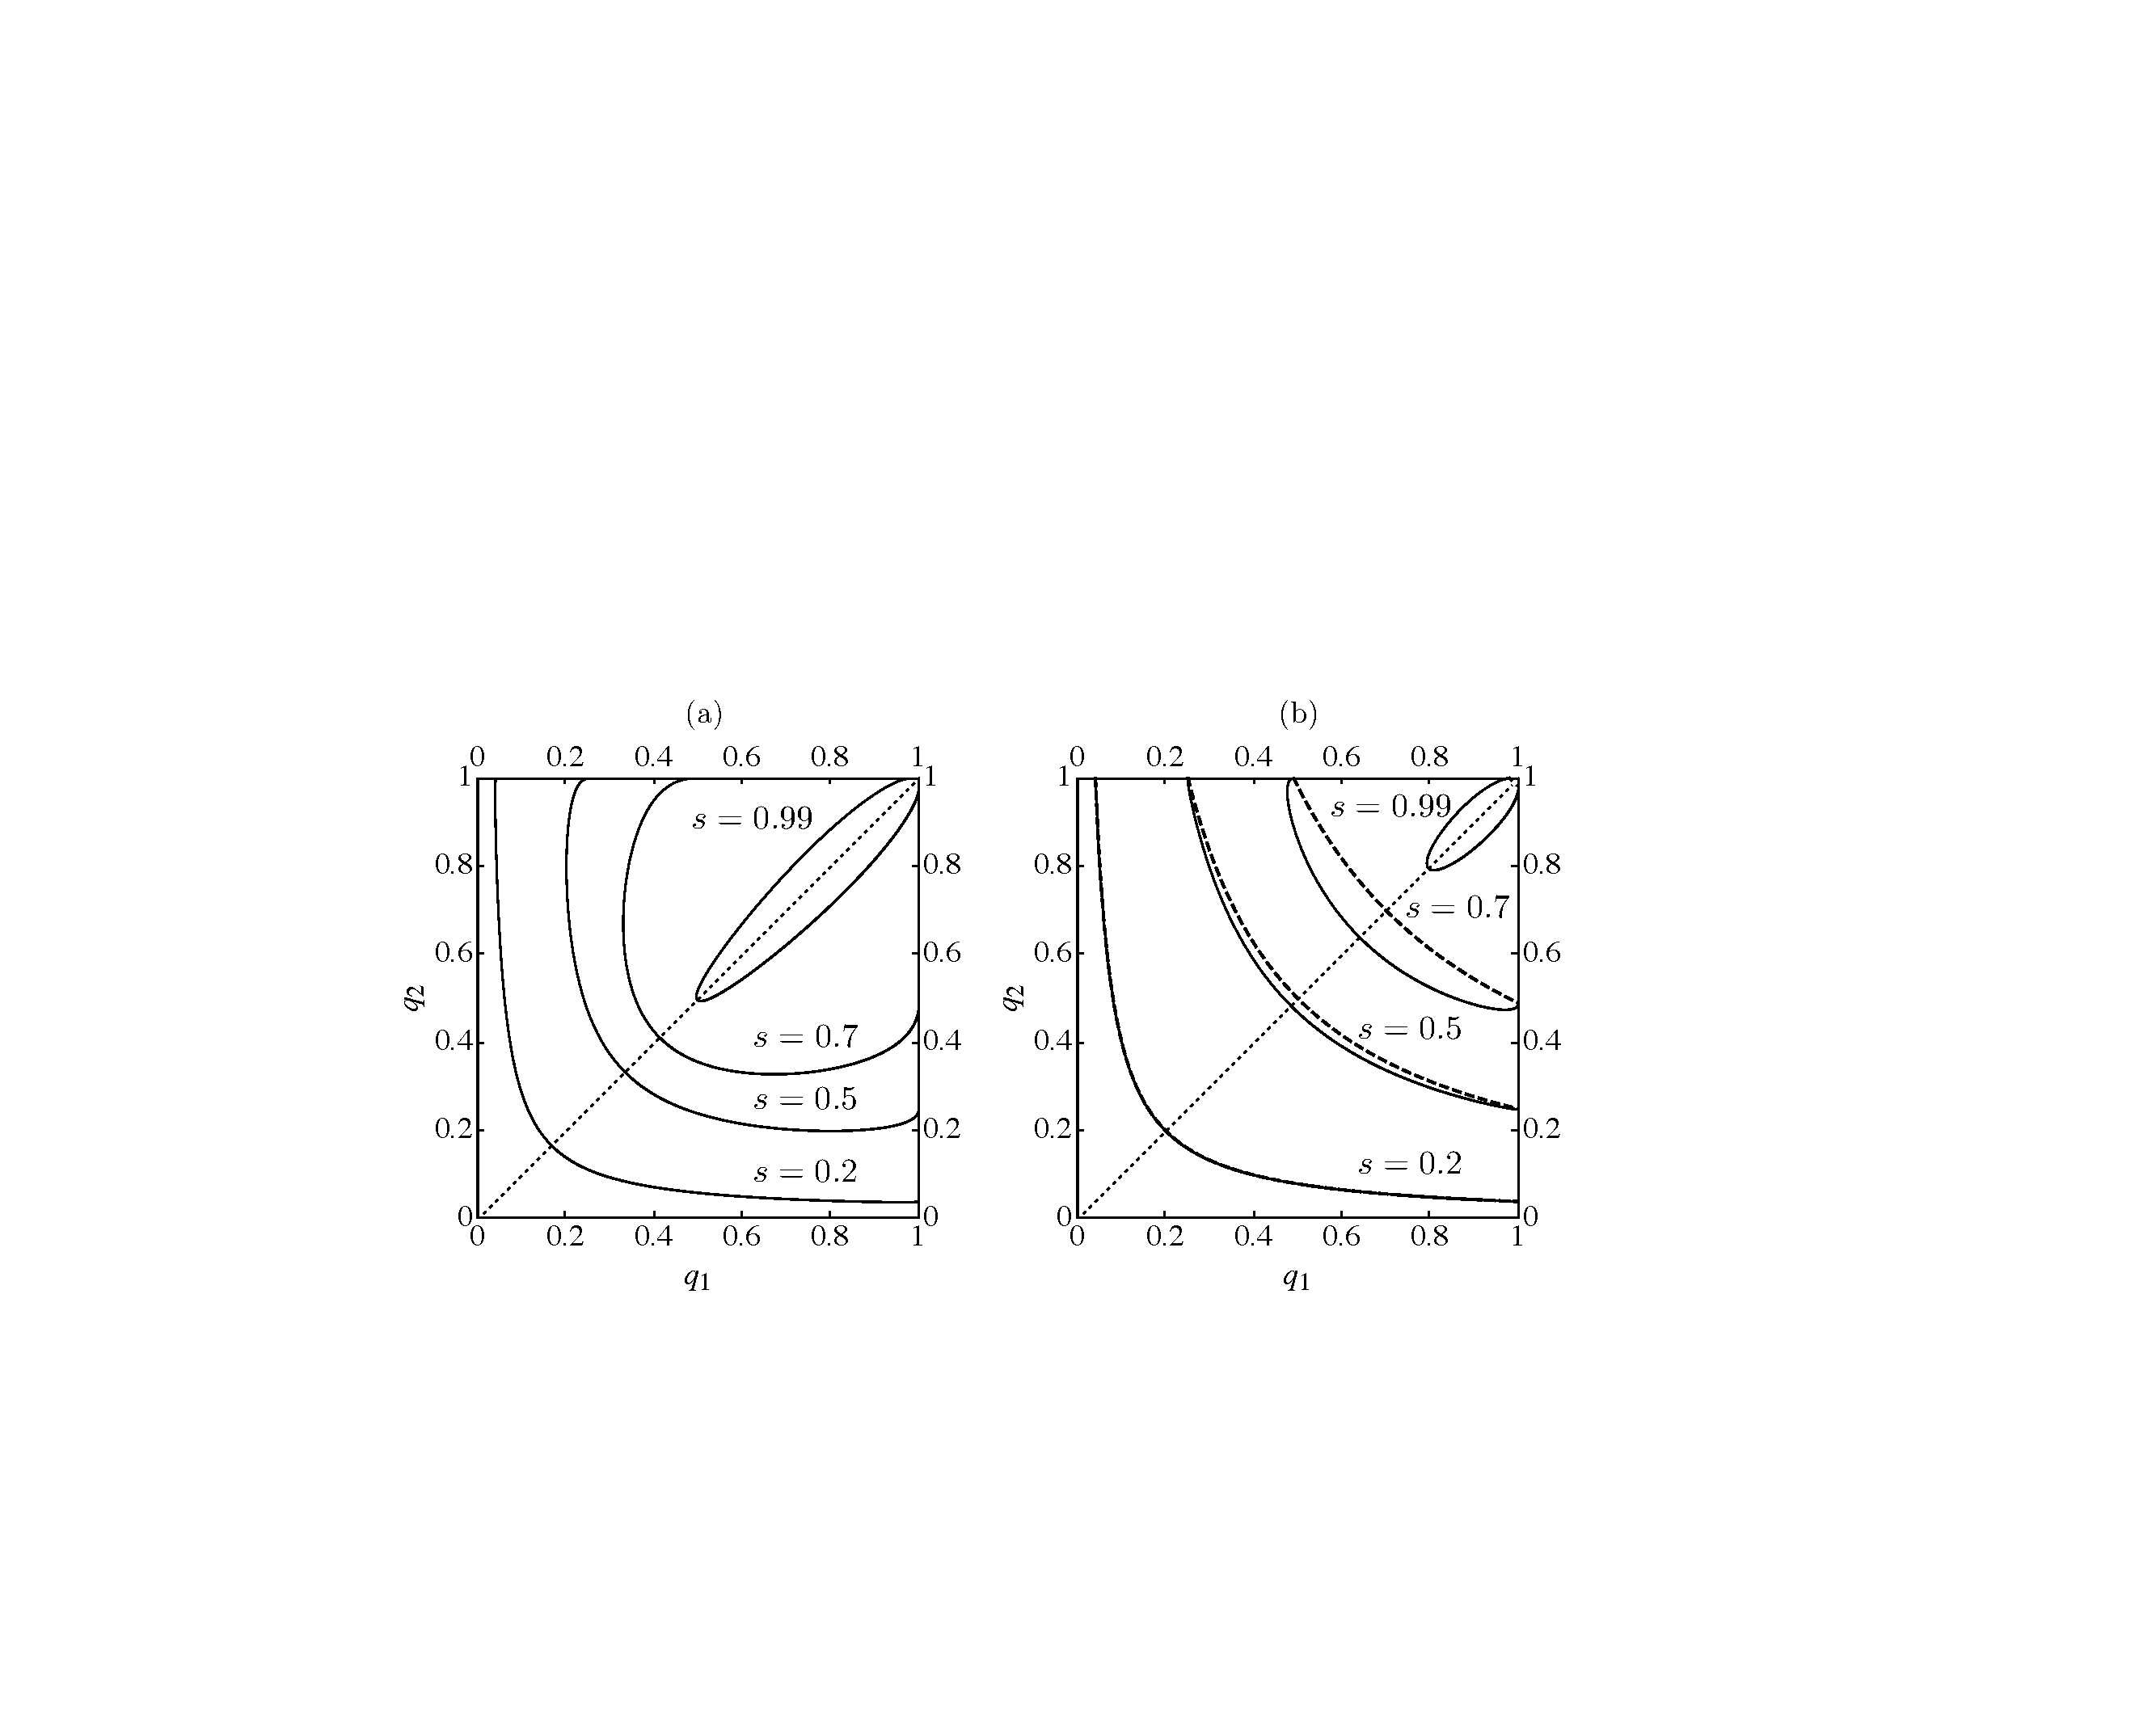
\includegraphics[width=26.8em]{Fig_2NC.pdf}\\
\end{array}%
$%
\caption{Unitarity curves, $q_{2}$ vs. $q_{1}$, from Eq.~(\ref{unit cond}) for different values of~$s$ and for (a) $m=1$, $n=2$ and (b) $m=1$, $n=5$. The curves are symmetric under mirror reflection along the dotted line $q_1=q_2$, i.e., under the transformation~$q_1\leftrightarrow q_2$. The dashed lines in~(b) are the hyperbolae~$q_1 q_2=s^{2m}$.}
\label{fig:2}
\end{figure}

For $n > 2$ the curves closely approximate  {\color{blue} $q_1 q_2=s^{2m}$} (dashed lines) for small and moderate values of $s$, while for $s$ close to $1$ the hyperbolas remain closer to the vertex~$(1,1)$, but retain the same end points. In the limit $n\to\infty$ all  {\color{blue} these} curves become hyperbolic.

We now return to finding the minimum, $Q_{\rm min}$, of the average failure probability $Q$. Despite its apparent simplicity, this involves solving a high-order equation without a simple form. Instead, we will derive a parametric equation for {\color{red}$Q_{\rm min}(\eta_1)$}. Along with the complete description of the unitary curve~(\ref{unit cond}), this provides a complete solution of the problem in parametric form.

With no loss of generality we may assume $\eta_1\le\eta_2$ or, equivalently,  $0\le\eta_1\le 1/2$. Then the slope of the straight line~(\ref{obj fun}), $-\eta_{1}/ \eta_{2}$, satisfies $-1\leq -\eta_{1}/\eta_{2} \leq0$. Hence, it can only become tangent to the lower half of the unitarity curve~(\ref{unit cond}) (see Fig.~\ref{fig:2}). %It is apparent from Fig.~\ref{fig:2} that 
Increasing $q_{1}$, the slope of this lower half increases monotonically from $-1$ at $q_1=q_2$, to $0$ before we reach the line~$q_1=1$. This follows from the properties (a)--(f) above and can be checked using  Eq.~(\ref{par sqrt}). The values of $t$ at which the slope is $-1$ and $0$ are, respectively,
%
\begin{equation}
t_{-1}=\frac{1-s^{n-m}}{1-s^n},\quad
t_0=\frac{1-s^{2(n-m)}}{1-s^{2n}}.
\label{t's}
\end{equation}
%
%where we note that $t_{-1}$ is the lower value of the range of~$t$ in Eq.~(\ref{range t}). 
For any point $(q_1(t),q_2(t))$ with $t\in[t_{-1},t_0]$ there is a line $Q=\eta_1 q_1+\eta_2 q_2$ that is tangent to it, starting with $\eta_1=\eta_2=1/2$ for $t=t_{-1}$ up to $\eta_1=0$, $\eta_2=1$ for $t=t_0$. 

This observation enables us to derive the desired parametric expression for the optimality curve~$Q_{\rm min}(\eta_1)$ as follows. For a given $t$ in the range above, a necessary condition for tangency is \mbox{$\eta_1 q'_1+\eta_2 q'_2=0$}, where $q'_i=d q_i/d t$. In this equation we can solve for $\eta_1$ (or $\eta_2$) using that~$\eta_1+\eta_2=1$. By substituting $q_1$ and~$q_2$ in Eq.~(\ref{obj fun}) with~(\ref{par sqrt}) we enforce contact with the unitarity curve and obtain the expression of $Q_{\rm min}$. The final result can be cast as:
%
\begin{equation}
\eta_1=\frac{q'_2}{q'_2-q'_1},\;\; Q_{\rm min}=\frac{q'_2 q_1-q'_1 q_2}{q'_2-q'_1},\;\; t_{-1}\le t\le t_0,
\label{main}
\end{equation}
%
where $t_{-1}$, $t_0$ and $q_i$ are given in Eqs.~(\ref{t's}) and~(\ref{par sqrt}). The expressions for the derivatives $q'_i$ are %most easily derived from the trigonometric form~(\ref{par trig}) to be
%
\begin{equation}
q'_i=\frac{\sqrt{q_i(1-q_i)}}{s^{n-m}}\left\{\frac{1+s^n}{\sqrt{1-x^2}}-(-1)^i\frac{1-s^n}{\sqrt{1-y^2}}\right\}.
\end{equation}
%

Fig.~\ref{fig:3} shows plots of the curves $Q_{\rm min}(\eta_1)$ for $m=1$ input copies and  (a) $n=2$ or (b) $n=5$ clones, as in the previous figure. We see that $Q_{\rm min}$ is an increasing function of $\eta_1$ in the given range $[0,1/2]$. The values of~$Q_{\rm min}$ at the end points of this range follow by substituting $t_{0}$ and $t_{-1}$, Eq.~(\ref{t's}), into Eq.~(\ref{par sqrt}). They are given by
%
\begin{equation}
Q_{0}=q_2(t_0)=\frac{s^{2m}-s^{2n}}{1-s^{2n}},\quad
Q_{-1}=\frac{s^m-s^n}{1-s^n},
\label{Q's}
\end{equation}
%
where $Q_{\rm min}=Q_{-1}$ holds for equal priors and $Q_{\rm min}=Q_0$ for $\eta_1\to 0$ (i.e., $\eta_2\to 1$).
\begin{figure}[ht]
\centering
$%
\begin{array}{c}
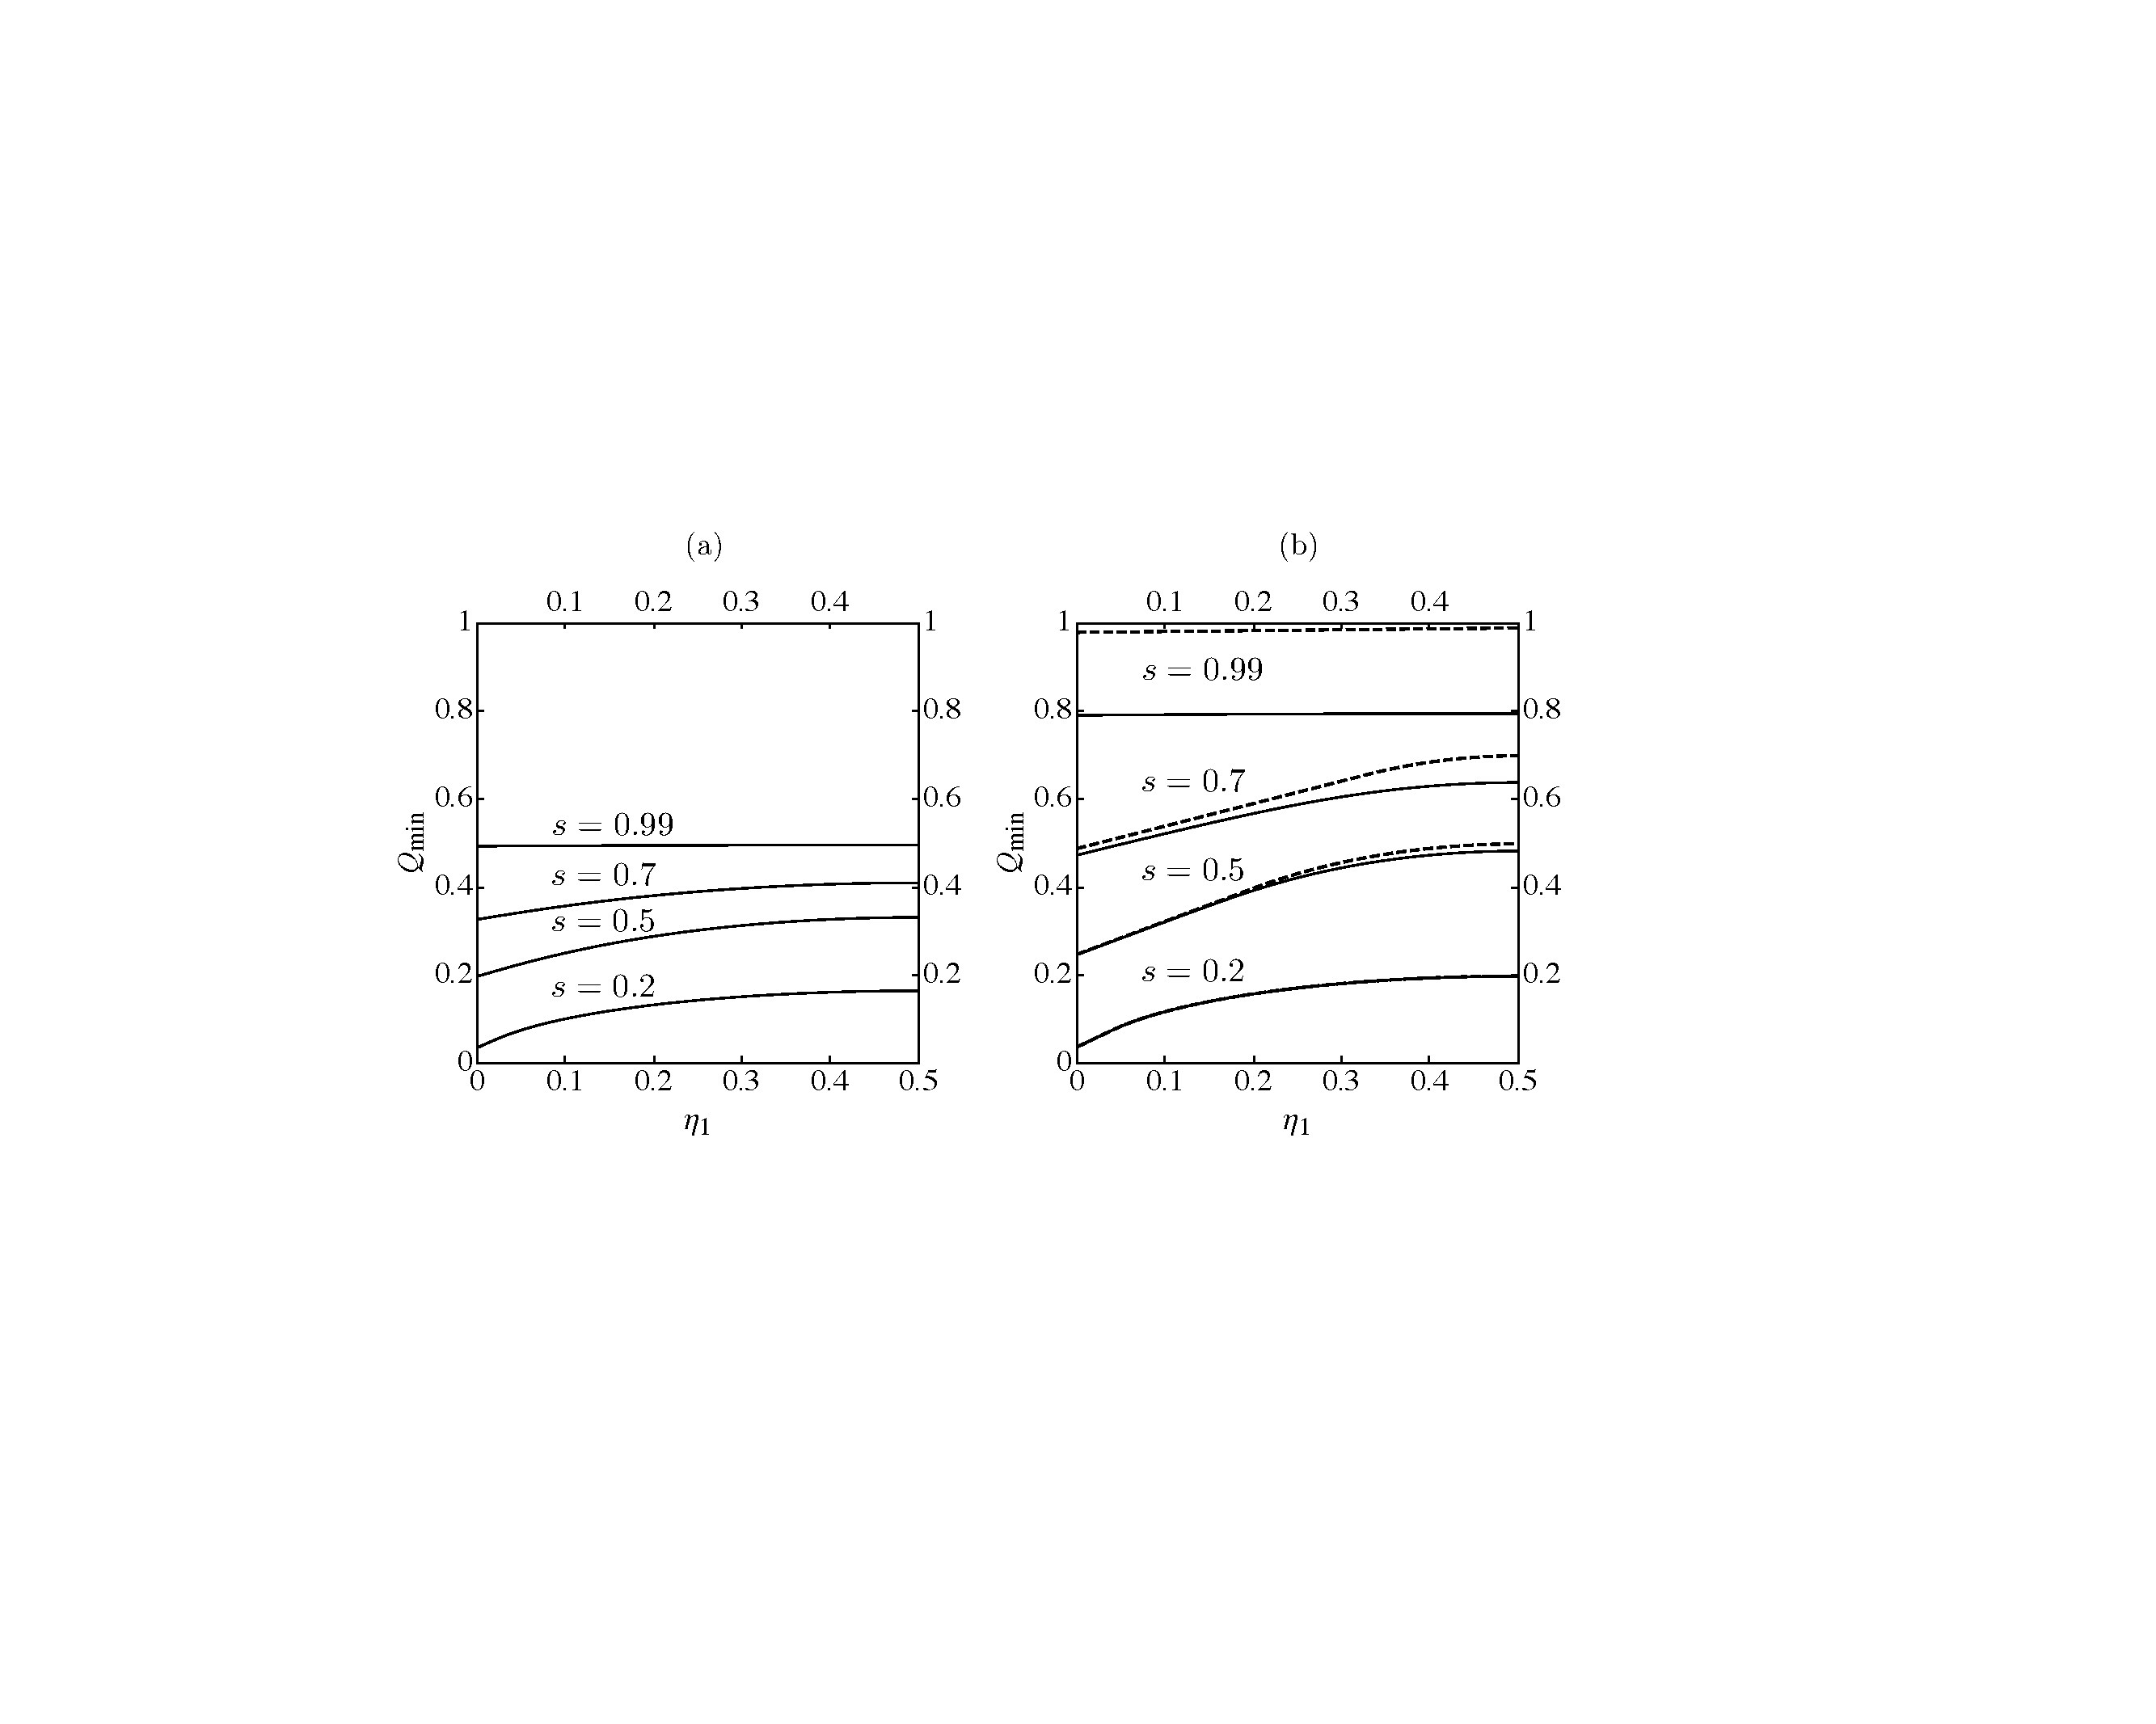
\includegraphics[width=26.7em]{Fig_3NC.pdf}\\
\end{array}%
$%
\caption{Minimum cloning failure probability $Q_{\rm min}$ vs. $\eta_1$ (solid lines) and~UD failure probability $Q_{\rm UD}$ vs. $\eta_1$ (dashed lines) for the same values of $m$, $n$ and $s$ used in the previous figure.}
\label{fig:3}
\end{figure}
The dashed lines in Fig.~\ref{fig:3}~(b) depict the well known optimal UD solution~\cite{Bergou}:
%
\begin{equation}
Q_{\rm UD}=\left\{
\begin{array}{ll}
2\sqrt{\eta_1\eta_2}\, s^m,&\displaystyle \frac{s^{2m}}{1+s^{2m}}\le\eta_1\le \frac{1}{2};\\[.5em]
\eta_1+s^{2m} \eta_2, \quad &\displaystyle 0\le \eta_1\le \frac{s^{2m}}{1+s^{2m}}.
\end{array}
\right.
\label{UD}
\end{equation}
%

It is apparent from these plots that the optimal cloning protocol performs strictly better than cloning by discrimination, as was geometricaly proved in Figs. \ref{fig:1} and \ref{fig:2}. However, the difference in performance decreases with increasing number of clones. In Fig.~\ref{fig:3}~(b), for only $n=5$, a difference is hardly noticeable for $s\le 0.5$. For $s > 0.5$ the convergence is slower but in the limit $n\to\infty$ there is perfect agreement for any $s<1$.

{\color{red}%The complete UD solution in Eq.~(\ref{UD}) 

The convergence of the optimal cloning failure probability, $Q_{\rm min}$, to that of cloning by discrimination, $Q_{\rm UD}$ in Eq.~(\ref{UD})
follows from our geometrical approach. Recall that in the limit $n\to\infty$ (or equivalently $\alpha\to0$)  the right hand side of Eq.~(\ref{unit cond}) describes hyperbolas that we can write as $q_2=s^{2m}/q_1$ (dashed lines in Figs.~\ref{fig:1} and~\ref{fig:2}). Their  {\color{blue}slopes are} in the range $[-1,-s^{2n}]$.  A unique point of tangency with the line~(\ref{obj fun}) can only exists if the slope of this line, $-\eta_1/\eta_2$, is within this same range. This gives the $\eta_1$ interval in the first line of~(\ref{UD}), and one can easily obtain the corresponding expression for~$Q_{\rm UD}$.
%
If the slope of the line~(\ref{obj fun}) is outside the range, tangency is not possible, and the optimal line merely touches the end points of the hyperbolas, so the expression of~$Q_{\rm UD}$ becomes the second line of Eq.~(\ref{UD}). In geometrical terms, the straight line~(\ref{obj fun}) pivots on the end points as we vary~$\eta_1$. Furthermore, note that for the second line in~(\ref{UD}) we have $p_1=1-q_1=0$, which leads to a $2$-outcome projective measurement, as only one success flag state ($|\alpha_2\rangle$) is needed in Eqs.~(\ref{Ui}). 
%
%
%$s^{2m}<\eta_1/\eta_2\le1$, leading the optimal failure rate in the second line of Eq.~(\ref{UD}).  For $0 \leq \eta_1 \leq s^{2m}/(1+s^{2m})$, the straight line~(\ref{obj fun}) pivots on the end point $(1,s^{2m})$, producing the first line of the solution.

Interestingly, in this limit a phenomenon analogous to a second order phase transition takes place. Our geometrical approach shows that the average failure probability $Q_{\rm min}(\eta_1)$ is an infinitely differentiable function of~$\eta_1$ for finite $n$. However, as $n$ goes to infinity (corresponding to $\alpha=0$) the limiting function $Q_{\rm UD}(\eta_1)$ has a discontinuous second derivative. Moreover, the symmetry $q_1\leftrightarrow q_2$ breaks  in the ``phase" corresponding to the first line in Eq.~(\ref{UD}). A~similar phenomenon arises in UD of more than two pure states~\cite{Bergou1}.}

%In the limit  $Q_{\rm min} \to Q_{\rm UD}$ a phenomenon analogous to a second order phase transition takes place. Our geometrical approach shows that the average failure probability $Q_{\rm min}(\eta_1)$ is an infinitely differentiable function of~$\eta_1$ for finite $n$. However, as $n$ goes to infinity (corresponding to $\alpha=0$) the limiting function $Q_{\rm UD}(\eta_1)$ has a discontinuous second derivative. Moreover, the symmetry $q_1\leftrightarrow q_2$ breaks  in the ``phase" corresponding to the first line in Eq.~(\ref{UD}). A~similar phenomenon arises in UD of more than two pure states~\cite{Bergou1}.

%The complete UD solution in Eq.~(\ref{UD}) emerges from our geometrical approach in a straightforward manner. First, we recall that in this case the right hand side of Eq.~(\ref{unit cond}) becomes $q_1 q_2=s^{2m}$ (dashed lines in Figs.~\ref{fig:1} and~\ref{fig:2}). The maximum slopes of these curves are at their end points and all have the value~$-s^{2m}$. This implies that the boundary of $S_0$ has a cusp at $(1,s^{2m})$. It follows that a unique point of tangency with the line~(\ref{obj fun}) exists for $s^{2m}<\eta_1/\eta_2\le1$ (recall that we are assuming~$\eta_1\le1/2$). This condition gives the $\eta_1$ interval for that solution.  At the point of tangency, the normal vectors of the two curves are parallel, $(q_2,q_1)\propto (\eta_1,\eta_2)$, leading to the optimal failure rate in the second line of Eq.~(\ref{UD}). For $s^{2m}>\eta_1/\eta_2\ge0$ tangency is not possible, and the optimal line~(\ref{obj fun}) merely touches the cusp on the boundary of~$S_0$, so the expression of $Q$ becomes the first line of Eq.~(\ref{UD}). In geometrical terms, the straight line~(\ref{obj fun}) pivots on the end point for $0 \leq \eta_1 \leq s^{2m}/(1+s^{2m})$.
%
%For the second case in Eq.~(\ref{UD}), one has $q_1,p_1\in(0,1)$ and there are three orthogonal flag states in Eqs.~(\ref{Ui}), the success states $|\alpha_1\rangle$, $|\alpha_2\rangle$, and the failure state~$|\alpha_{0}\rangle$. This $3$-outcome measurement can be represented by a $3$-element positive operator valued measure (POVM) on ${\mathscr H}^{\otimes m}$. For the first line in Eq.~(\ref{UD}), $p_1=1-q_1=0$, which leads to a $2$-outcome projective measurement, as only one success flag state ($|\alpha_2\rangle$) is needed in Eqs.~(\ref{Ui}). 

%This short re-derivation of Eq.~(\ref{UD}) proves the convergence of the optimal cloning failure probability, $Q_{\rm min}$, to that of cloning by discrimination, $Q_{\rm UD}$ in Eq.~(\ref{UD}). It follows from the convergence of the general unitarity curve in Eq.~(\ref{unit cond}) to the hyperbola $q_1q_2=s^{2m}$, i.e., from $\lim_{{\mathrm n}\to 0} S_\alpha=S_0$. 

%It has been argued above that cloning by discrimination is strictly suboptimal (unless $n\to \infty$). 
%One could likewise wonder if discrimination by cloning can be optimal. On heuristic grounds, one should not expect this to be so, as cloning involves a measurement and some information can be drawn from the observed outcome. However, the equal-prior and the $\eta_1\to 0$ cases provide remarkable exceptions: for $\eta_1 = \eta_2= 1/2$, cloning succeeds with probability $P=1-Q_{-1}$, in which case the produced $n$-clone states are equally likely. The UD of these estates fails with probability $s^{n}$, as follows from Eq.~(\ref{UD}) applied to $n$ copies. The total failure probability is then $Q_{-1}+P s^n=s^m$, which is the optimal UD failure rate of the original input states, Eq.~(\ref{UD}). 
%If  $\eta_1\to 0$ then $P=1-Q_{0}$, and only $|\psi^n_2\rangle$ is produced with non-vanishing probability. Failure in the second step (UD) is given by Eq.~(\ref{UD}) applied to $n$ copies. The total failure rate is $Q_{0}+P s^{2n}=s^{2m}$, also achieving optimality. 

It has been argued above that cloning by discrimination is strictly suboptimal (unless $n\to \infty$).
One could likewise wonder if discrimination by cloning can be optimal. On heuristic grounds, one should not expect this to be so, as cloning involves a measurement and some information can be drawn from the observed outcome. However, the equal-prior and the $\eta_1\to 0$ cases provide remarkable exceptions. For both we may write the total failure rate as $Q_{\rm C} + (1-Q_{\rm C})Q_{\rm UD}$, where C stands for cloning. For $\eta_1 = \eta_2= 1/2$, Eq.~(\ref{Q's}) implies $Q_{\rm C}=Q_{-1}$, in which case the produced $n$-clone states are equally likely. The UD of these states fails with probability $s^{n}$, as follows from Eq.~(\ref{UD}) applied to $n$ copies. The total failure rate is then $s^m$, which is the optimal UD failure rate of the original input states, Eq.~(\ref{UD}). If $\eta_1\to 0$ then only $|\psi^n_2\rangle$ is produced with non-vanishing probability and  $Q_{\rm C}=Q_{0}$. Failure in the second step (UD) is given by the top line in Eq.~(\ref{UD}) applied to $n$ copies. The total failure rate is $s^{2m}$, also achieving optimality. 

Using our main result in Eqs.~(\ref{main}), and~(\ref{par sqrt}) one can check that these are the only cases where discrimination by cloning is optimal. These are also the only cases where no information gain can be drawn from the cloning measurement.  This hints at how special these cases are and justifies the need of the derived solution for arbitrary priors to have a full account of two-state cloning. 

%%%%%%%%%%%%%%%%%%%%%%%%%%%%%%%%%%%%%%%%%%%%%%%%
%%%%%%%%%%%%%%%%%%%%%%%%%%%%%%%%%%%%%%%%%%%%%%%%
\subsection{Equal priors. }

%%%%%%%%%%%%%%%%%%%%%%%%%%%%%%%%%%%%%%%%%%%%%%%%
%%%%%%%%%%%%%%%%%%%%%%%%%%%%%%%%%%%%%%%%%%%%%%%%
\subsection{Unequal priors I}


%%%%%%%%%%%%%%%%%%%%%%%%%%%%%%%%%%%%%%%%%%%%%%%%
%%%%%%%%%%%%%%%%%%%%%%%%%%%%%%%%%%%%%%%%%%%%%%%%
\subsection{Unequal priors II}




%%%%%%%%%%%%%%%%%%%%%%%%%%%%%%%%%%%%%%%%%%%%%%%%
%%%%%%%%%%%%%%%%%%%%%%%%%%%%%%%%%%%%%%%%%%%%%%%%
\section{Exact Cloning then Unambiguous Discrimination. *RENAME* }




%%%%%%%%%%%%%%%%%%%%%%%%%%%%%%%%%%%%%%%%%%%%%%%%
%%%%%%%%%%%%%%%%%%%%%%%%%%%%%%%%%%%%%%%%%%%%%%%%
\section{Hybrid Cloning: Interpolation between exact and approximate cloning }


%%%%%%%%%%%%%%%%%%%%%%%%%%%%%%%%%%%%%%%%%%%%%%%%
%%%%%%%%%%%%%%%%%%%%%%%%%%%%%%%%%%%%%%%%%%%%%%%%
\subsection{Equal priors}


%%%%%%%%%%%%%%%%%%%%%%%%%%%%%%%%%%%%%%%%%%%%%%%%
%%%%%%%%%%%%%%%%%%%%%%%%%%%%%%%%%%%%%%%%%%%%%%%%
\subsection{General case}



%%%%%%%%%%%%%%%%%%%%%%%%%%%%%%%%%%%%%%%%%%%%%%%%
%%%%%%%%%%%%%%%%%%%%%%%%%%%%%%%%%%%%%%%%%%%%%%%%
%%%%%%%%%%%%%%%%%%%%%%%%%%%%%%%%%%%%%%%%%%%%%%%%
%%%%%%%%%%%%%%%%%%%%%%%%%%%%%%%%%%%%%%%%%%%%%%%%
\chapter{State Separation}

We can always imagine that a probabilistic quantum transformation is carried out by a machine with an input port, an output port and two flags that herald the success or failure of the transformation.  The input $|\psi_i\rangle$, $i=1,2$ is fed through the input port for processing. In case of success, states~$|\psi'_i\rangle$, with the desired degree of separation, are delivered through the output port with conditioned probability~$p_i$. Otherwise, the output is in a failure state. Conditioned on the input state being $|\psi_i\rangle$, the failure probability is~$q_i=1-p_i$. 

We address optimality from a Bayesian viewpoint that assumes the states to be transformed are given with some {\it a priori}  probabilities $\eta_1$ and $\eta_2$, $\eta_1+\eta_2=1$. Then a natural cost function for our probabilistic machines is given by the average failure probability 
%
\begin{equation}
Q=\eta_1 q_1+\eta_2 q_2.
\label{obj fun}
\end{equation}
%
If $|\psi_i\rangle$ and the corresponding transformed states $|\psi'_i\rangle$ are given, the optimal machine is one that minimizes the cost function 
%Accordingly, the optimal cloner is one that minimizes the cost function 
$Q$. In this case our aim is to find that optimal machine and the minimum average failure probability $Q_{\rm min}$ for arbitrary priors $\eta_1$ and $\eta_2$.
% This does {\em not} define a universal protocol. 
%The information about the two possible state preparations $|\psi_i\rangle$, their corresponding prior probabilities $\eta_i$, $i=1,2$, and transformed states~$|\psi'_i\rangle$ is hardwired into the machine. 

A different way of approaching optimality may consist in finding the machine (or machines) that achieves the highest degree of separation, namely, minimizes de overlap $s':=|\langle\psi'_1|\psi'_2\rangle|$ for given initial states $|\psi_i\rangle$, subject to the condition that the average probability~$Q$ does not exceed some given value, $Q_{\rm max}$. In this case we could further assume that either the initial overlap $s:=|\langle\psi_1|\psi_2\rangle|$ is given, in which case one can compute the tradeoff curve~$s'_{\rm min}(Q_{\rm max})$, or else assume that $Q_{\rm max}$ is fixed and compute the curve~$s'_{\min}(s)$. It is easy to see that $s'_{\rm min}(Q_{\rm max})$ and $Q_{\rm max}(s'_{\rm min})$ are just inverses of each otrher.

Whether we approach optimality one way or another depends merely on the problem at hand. Hence, e.g., for perfect cloning from one initial copies of either $|\psi_1\rangle$ or~$|\psi_2\rangle$ to $n$ final copies (i.e., $|\psi'_i\rangle=|\psi_i\rangle^{\otimes n}$), the former approach is most suitable since the final overlap is fixed, $s'=s^n$,  and so is the degree of separation attained by the cloner. So, in~\cite{us1} the solution was given in terms of~$Q_{\rm min}$ as a function of the prior probability $\eta_1$. However, one may need to know what is the maximum number of clones that can be produced if the failure rate cannot exceed~$Q_{\rm max}$, in which case one takes the latter approach, and compute $n_{\rm max}=\log[s'(Q_{\rm max})]/\log s$. 

The machine that carries the probabilistic transformation is usually described by two Kraus operators $A_{\rm succ}$, $A_{\rm fail}$, so that~$A^\dagger{}_{\kern-.3em\rm succ}A_{\rm succ}+A^\dagger{}_{\kern-.2em\rm fail}A_{\rm fail}=$~\cite{Chefles+Barnett}. We can think of $A_{\rm succ}$ and $A_{\rm fail}$ as measurement operators. The transformation is successfully applied if the outcome of such (generalized) measurement is ``succ",  and fails otherwise.
Neumark's theorem provides an alternative approach  that turns out to be more convenient for our analysis.  Additional details on this method can be found in \cite{Bergou}. 
In this formulation, %similar to that in~\cite{DuanGuo}, 
the Hilbert space ${\mathscr H}$ of the original states is supplemented with an ancillary space~${\mathscr H}_{\rm extra}\otimes {\mathscr H}_F$ that accommodates both the required extra-dimensions (if necessary) as well as the success/failure flags. Then, a unitary transformation~$U$ (time evolution) from ${\mathscr H}\otimes {\mathscr H}_{\rm extra}\otimes {\mathscr H}_{F}$ onto ${\mathscr H}'\otimes{\mathscr H}_F$ is defined through~\cite{DuanGuo}
%
\begin{eqnarray}
U|\psi_1\rangle|0\rangle&=& \sqrt{p_1}|\psi'_1\rangle|\alpha_1\rangle +\sqrt q_1 |\phi\rangle|\alpha_0\rangle,\label{U1}\\
U|\psi_2\rangle|0\rangle&=& \sqrt{p_2}|\psi'_2\rangle|\alpha_2\rangle +\sqrt q_2 |\phi\rangle|\alpha_0\rangle. \label{U2}
\end{eqnarray}
%
Here the ancillas are initialized in a reference state~$|0\rangle$. The states of the flag associated with successful transformation~$| {\alpha_i}\rangle$ are constrained to be orthogonal to the state~$|\alpha_0\rangle$ that signals failure. Upon performing a projective measurement  on the flag space ${\mathscr H}_F$, the final state delivered through the outport port of our probabilistic machine is either $|\psi'_i\rangle$, in case of success, or $|\phi\rangle$ in case of failure. So, the outcome of this measurement tells us if the machine has succeeded or failed in delivering the right transformed state.  On general grounds, optimality requires $|\alpha_1\rangle=|\alpha_2\rangle$. Here we choose to consider a more general setup where these two states are different
to include state discrimination, for which the success flag states must be fully distinguishable, so $\langle\alpha_1|\alpha_2\rangle=0$.
%
Likewise, we could consider a more general setup with two failure states $|\phi_1\rangle$ and $|\phi_2\rangle$ in Eqs.~(\ref{U1}) and~(\ref{U2}). This is necessarily sub-optimal since we could probabilistically determine whether we received $|{\psi_1}\rangle$ or $|{\psi_2}\rangle$ by applying unambiguous discrimination to the failure states~$| {\phi_i}\rangle$.  Sometimes we would be  certain of the input state, in which case we could  prepare $|\psi'_1\rangle$ or $|\psi'_2\rangle$ accordingly,  thereby increasing the overall success rate.
%
%

%From our analysis the optimality requirement $|\alpha_1\rangle=|\alpha_2\rangle$ will trivially follow.
Taking the inner product of Eqs.~(\ref{U1}) and ~(\ref{U2}) with themselves shows that our probabilities are normalized: $p_i+q_i=1$.
Similarly, by taking the product of Eq.~(\ref{U1}) with Eq.~(\ref{U2}), we find the unitarity constraint,
%
\begin{equation}
s=\sqrt{p_1 p_2}\, \beta+\sqrt{q_1 q_2},
\label{unit cond}
\end{equation}
%
where $\beta=s' |\langle \alpha_1|\alpha_2\rangle|$. Without any loss of generality, in deriving Eq.~(\ref{unit cond}) we have chosen
$\langle {\psi_1}|{\psi_2}\rangle$, $\langle {\psi'_1}|{\psi'_2}\rangle$ and~$\langle\alpha_1|\alpha_2\rangle$ to be real and positive.
%~\footnote{%
%
%
%We may choose $\alpha$ (and $\langle\Phi_1|\Phi_2\rangle=\phi$) to be real, since only their real parts show up in the unitarity condition, Eq.~(\ref{unit cond}), and the additional condition
%$$
%0=\sqrt{p_1p_2}s' \Im\,\alpha+\sqrt{q_1q_2}\Im\,\phi
%$$
%is satisfied by the choice $ \Im\,\alpha=\Im\,\phi=0$.%
%%
%%
%}
%. 
%Furthermore, we can choose $0\le s'\le s\le 1$.  
We note that $0\le\beta\le s$, and~$\beta=0$ for both full separation ($s'=0$) and unambiguous discrimination ($ |\langle \alpha_1|\alpha_2\rangle|=0$), whereas for optimal separation~$|\langle \alpha_1|\alpha_2\rangle|=1$. If Eq.~(\ref{unit cond}) is satisfied, it is not hard to prove that~$U$ has a unitary extension on the whole Hilbert space and the Kraus operators,~\mbox{$A_{\rm succ}$, $A_{\rm fail}$,} can be obtained by tracing out the ancillary degrees of freedom .

\begin{figure}[t]
\centering
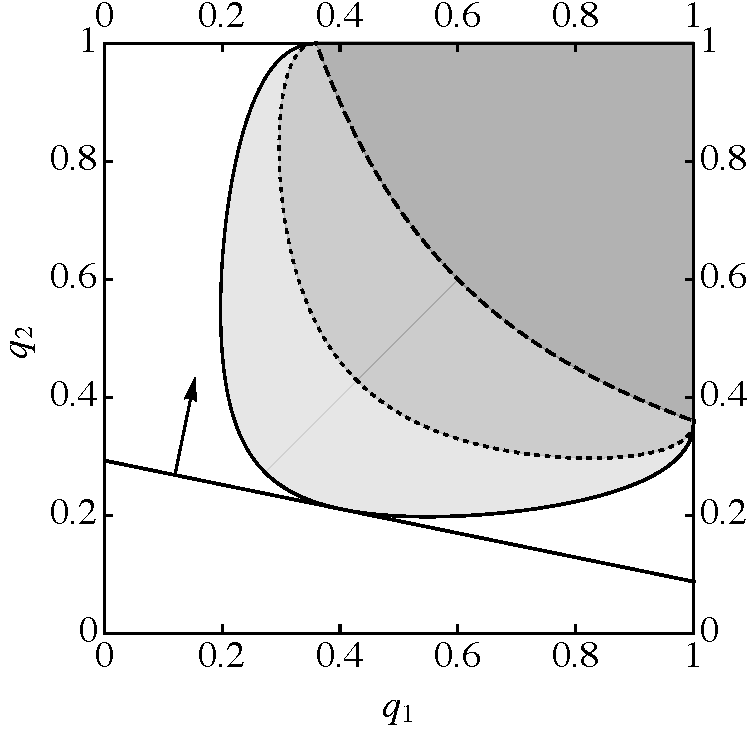
\includegraphics[width=14em]{Separation_F0.pdf}
%
\caption{Unitarity curves in Eq.~(\ref{unit cond}) and the associated sets~$S_\beta$ %, where $\beta= s'|\langle\alpha_1|\alpha_2\rangle|$, 
in Eq.~(\ref{S_alpha}) for $\beta=0.45$ (solid/light~gray), $\beta=0.30$ (dotted/medium gray), and $\beta=0$ (dashed/dark gray). The figure also shows the optimal straight segment \mbox{$Q=\eta_1 q_1+\eta_2 q_2$} and its normal vector~$(\eta_1,\eta_2)$. Plotted for  $s = 0.6$, $\eta_1=0.17$, $\eta_2=0.83$ and~$Q=0.24$.}
\label{fig:1}
\end{figure}


%{\color{red}In the following lemma we gather all the features of the unitary constraint (some of them straightforward)  that provide geometric insight into our optimization problem.}
{\color{blue}For convenient referencing, we gather in a lemma all the features of the unitary constraint that we will need.  Points (a)--(d) are straightforward, so only (e) and (f) are proven below.}

\begin{lemma}
(a)~For fixed $s$, Eq.~(\ref{unit cond}) defines a class of smooth curves on the unit square {\color{red}$0< q_i< 1$} (e.g., solid, dashed or dotted curves in Fig.~\ref{fig:1}). (b)~All these curves meet at their endpoints, $(1,s^{2})$ and $(s^{2},1)$. (c)~At the endpoints  the curves become tangent to the vertical and horizontal lines~$q_1=1$ and~$q_2=1$ respectively, provided~$\beta$ is not zero. %This is due to the square root $\sqrt{p_1p_2}$ in Eq.~(\ref{unit cond}).
%A more detailed analysis shows that f
(d)~For~$\beta=0$ the curve %defined by Eq.~(\ref{unit cond}) 
is an arc of the hyperbola $q_1 q_2=s^{2}$ (dashed line in Fig.~\ref{fig:1}). 
%
(e)~Each of these curves and the segments joining their end points with the vertex~$(1,1)$ enclose the sets (any of the gray regions in Fig.~\ref{fig:1})
%
\begin{equation}
S_\beta\!=\!\{ (q_1,\!q_2){\color{red}\in\![0,\!1]\!\times\![0,\!1]}:\!  \sqrt{p_1 p_2}\,\beta+\sqrt{q_1 q_2}-s\!\ge\! 0\}.
\vspace{1em}
\label{S_alpha}
\end{equation}
%
They satisfy $S_{\beta}\subset S_{\beta'}$ if $\beta<\beta'$.
(f)~Moreover, the sets~$S_\beta$ are convex. % if $\beta\ge0$ (i.e., if $\alpha\ge0$). In particular~$S_{s'}$ is convex.
%For $\alpha\ge0$ the set $S_\alpha$ is convex, as follows from the observation that~$(xy)^{1/2}$ is a concave function of its two (non-negative) arguments~$x$ and~$y$. 
\end{lemma}

\noindent{\bf Proof.} {\color{blue}(e)~The curve~(\ref{unit cond}) is readily seen to be part of the boundary of $S_\beta$. }%The segment joining $(1,s^2)$ with~$(1,1)$ is defined by $q_1=1$ and $q_2\ge s^2$, so it belong to $S_\beta$, and so does the segment joining $(s^2,1)$ with $(1,1)$.
Assume that~$\beta\le\beta'$ and $(q_1,q_2)\in S_\beta$. Then 
%
\begin{equation}
\sqrt{p_1 p_2}\,\beta'+\sqrt{q_1 q_2}-s\ge \sqrt{p_1 p_2}\,\beta+\sqrt{q_1 q_2}-s\ge0,
\end{equation}
%
and thus $(q_1,q_2)\in S_{\beta'}$. (f)~To prove convexity let us assume that $(q_1,q_2)$ and $(q'_1,q'_2)$ belong to $S_\beta$. We define $\bar q_i=\lambda q_i+(1-\lambda)q'_i$, where $0\le\lambda\le1$. It follows that $\bar p_i:=1-\bar q_i=\lambda p_i+(1-\lambda)p'_i$. Since~$f(x,y)=\sqrt{xy}$ is a concave function in the unit square $\{(x,y)\, |\, 0\le x,y\le 1\}$, we have $\sqrt{\bar q_1\bar q_2}\ge \lambda \sqrt{q_1q_2}+(1-\lambda)\sqrt{q'_1q'_2}$ and, since~$\beta\ge0$, $\sqrt{\bar p_1\bar p_2}\,\beta\ge \lambda \sqrt{p_1p_2}\,\beta+(1-\lambda)\sqrt{p'_1p'_2}\,\beta$. Then
%

\begin{equation}
\sqrt{\bar p_1 \bar p_2}\,\beta+\sqrt{\bar q_1 \bar q_2}-s\ge \lambda\left(\sqrt{p_1p_2}\beta+\sqrt{q_1q_2}-s\right)+(1-\lambda)\left(\sqrt{p'_1p'_2}\beta+\sqrt{q'_1q'_2}-s\right)\ge 0.
\end{equation}

%
Thus, $(\bar q_1,\bar q_2)\in S_\beta$, which proves the convexity of $S_\beta$ for~$\beta\ge0$.
$\blacksquare$

 Now that we have characterized the geometry of the unitarity constraint, a geometrical picture of the optimization problem emerges (See Fig.~\ref{fig:1}). 
Eq.~(\ref{obj fun}) defines a straight segment  on the square $0\le q_i\le 1$ with a normal vector in the first quadrant parallel to $(\eta_1,\eta_2)$. For fixed {\em a priori} probabilities, the average failure probability~$Q$ is proportional to the distance from this segment to the origin~$(0,0)$. The intersection of such a straight segment %~(\ref{obj fun}) 
with the boundary %~(\ref{unit cond}) 
of $S_\beta$ provides an admissible unitary transformation $U$ and its corresponding failure probability $Q$.
Since $S_{\beta}$ is convex and the stretch of its boundary given by Eq.~(\ref{unit cond}) is smooth, the optimal transformation, for which $Q$ is minimal, is defined by the unique point~$(q_1,q_2)$ of tangency with the segment~(\ref{obj fun}) that exists for any value of the priors and for $\beta>0$.
So, this tangency point determines the minimum failure probability $Q_{\rm min}$ and defines the optimal separation strategy through Eqs.~(\ref{U1}) and~(\ref{U2}). %(See Fig.~\ref{fig:1}). 

For $\beta=0$ (full separation/unambiguous discrimination),  the right hand side of Eq.~(\ref{unit cond}) describes hyperbolas that we can write as $q_2=s^{2}/q_1$ (dashed lines in Figs.~\ref{fig:1}). Their  slopes, $q'_2=-s^2/q_1^2$, are in the range~$[-s^{-2},-s^{2}]$.  A unique point of tangency with the line~(\ref{obj fun}) can only exists if the slope of this line,~$-\eta_1/\eta_2$, is within this same range, namely if $s^2/(1+s^2)\le \eta_1\le1/(1+s^2)$.
%%
%\begin{equation}
%{s^2\over1+s^2}\le\eta_1\le{1\over 1+s^2}.
%\end{equation}
%%
The tangency point is then seen to be $(q_1,q_2)=\sqrt{\eta_1\eta_2}\,s\, (\eta^{-1}_1,\eta^{-1}_2 )$. This leads to an minimum average failure probability given by {\color{red}$Q_{\rm min}=Q_{\rm UD}:=2\sqrt{\eta_1\eta_2}s$, where the subscript UD stands for unambiguous discrimination.}
%
If the slope is outside the range tangency is not possible, and then the optimal line merely touches the end points of the hyperbolas. For $\eta_1<s^2/(1+s^2)$, the straight segment~(\ref{obj fun}) pivots on the lower end point, $(1,s^2)$, as we vary~$\eta_1$ and we have the minimum average failure probability {\color{red}as} {\color{red}$Q_{\rm UD}=\eta_1+\eta_2 s^2$}. Likewise, for $\eta_1>1/(1+s^2)$, the pivoting point is the upper end point of the hyperbola, $(s^2,1)$, which leads to {\color{red}$Q_{\rm UD}=\eta_1 s^2+\eta_2$. The above can be summarized by
%
\begin{equation}
Q_{\rm UD}=\left\{
\begin{array}{ll}
2\sqrt{\eta_1\eta_2}\, s,&\displaystyle \frac{s^{2}}{1+s^{2}}\le\eta_1\le \frac{1}{1+s^{2}};\\[.8em]
\eta_1+s^{2} \eta_2, \quad &\displaystyle 0\le \eta_1\le \frac{s^{2}}{1+s^{2}};\\[.8em]
\eta_1 s^2+ \eta_2, \quad &\displaystyle \frac{1}{1+s^{2}}\le\eta_1\le  1.
\end{array}
\right.
\label{UD}
\end{equation}
%
}
We immediately recognize that this expression is the average failure probability of unambiguously discriminating the input states $|\psi_1\rangle$ and $|\psi_2\rangle$, as it was anticipated. 

Furthermore, we note that for the second (third) line in~(\ref{UD}) we have $p_1=1-q_1=0$ ($p_2=1-q_2=0$), which leads to a $2$-outcome projective measurement, as only the success flag state $|\alpha_2\rangle$  ($|\alpha_1\rangle$) is needed in Eqs.~(\ref{U1}) and~~(\ref{U2}). The solution in the first line of Eq.~(\ref{UD}) is manifestly symmetric under the exchange of the input states, i.e., under~$\eta_1\leftrightarrow\eta_2$. However, this symmetry is lost in the other lines. Instead,  the effect of swapping the states turns the solution in the second line of Eq.~(\ref{UD}) into the solution in the third line.  One can also check that~{\color{red}$Q_{\rm UD}$} is a twice differentiable function of $\eta_1$ (or $\eta_2$), with discontinuous second derivative at $\eta_1=s^2/(1+s^2)$ and $\eta_1=1/(1+s^2)$. Our geometrical approach shows that the average failure probability $Q_{\rm min}$ is an infinitely differentiable function of~$\eta_1$ for $\beta>0$, since according to our lemma, the boundary curve~(\ref{unit cond}) merges smoothly into the lines $q_1=1$ and $q_2=1$. 
%
So, it turns out that at $\beta=0$ a phenomenon similar to a second order symmetry breaking phase transition takes place. A~similar phenomenon was observed in unambiguous discrimination of more than two pure states~\cite{Bergou1}. 

Our lemma can likewise be used to address optimality for given priors~$\eta_1$ and~$\eta_2$ and average failure probability not exceeding~$Q_{\rm max}$, with $0\le Q_{\rm max}< {\color{red}Q_{\rm UD}}$. First, since the unitary curve is a function of~$\beta=s' \langle\alpha_1|\alpha_2\rangle$, we set $|\alpha_1\rangle=|\alpha_2\rangle$, i.e., $\langle\alpha_1|\alpha_2\rangle=1$, to ensure the minimum value of $s'>0$ for a given $\beta$. Then, it follows from the lemma that the minimum final overlap $s'>0$ (the maximum degree of separation attainable), which we call~$s'_{\rm min}$, is that for which the segment~(\ref{obj fun}), with $Q=Q_{\rm max}$, and the boundary of $S_{\beta=s'}$ become tangent. Setting the margin $Q_{\rm max}$ in the  range~{\color{red}$[Q_{\rm UD}, 1]$} leads, obviously, to the trivial solution $s'_{\rm min}=0$, for such margin would allow full separation using unambiguous discrimination with a failure rate of exactly {\color{red}$Q=Q_{\rm UD}$}, below the given margin. 
%The case $s'=0$, which is equivalent to unambiguous discrimination, is special and will be treated separately. We will show that state separation exhibits a second order phase transition at this particular value of output-state overlap.
%We note in passing that the inclusion hierarchy of the sets $S_\beta$ provides a simple geometrical proof that $\alpha=1$, i.e., $|\alpha_1\rangle=|\alpha_2\rangle$, is indeed the optimal choice.

In summary, our lemma provides the solution to optimal state separation from a geometrical viewpoint by showing that it is a convex optimization problem, for which a unique solution exists. Unfortunately,  a closed form for this solution does not exist for arbitrary prior probabilities, since finding the tangency point of the segment in Eq.~(\ref{obj fun}) with the curve in Eq.~(\ref{unit cond}) requires solving a six degree polynomial equation, as one can easily check. In the next sections, we give an analytic solution to state separation in parametric form. This solution contains all the information one may need in a simple and straightforward fashion. In particular, it enables us to easily draw plots of the relevant quantities for the various cases we will consider. 

%%%%%%%%%%%%%%%%%%%%%%%%%%%%%%%%%%%%%%%%%%%%%%%%
%%%%%%%%%%%%%%%%%%%%%%%%%%%%%%%%%%%%%%%%%%%%%%%%

\section{Minimum failure probability for a fixed degree of separation}\label{Q(eta)}

When the overlap of the final states is fixed, as in perfect cloning, we argued above that a natural problem consists in deriving the minimum failure rate of the optimal protocol, $Q_{\rm min}$, as a function of one of the priors, say $\eta_1$. In this section we address this problem by following the method employed in our derivation for cloning  in~\cite{us1}. All the expressions below can be obtained from their analogs in~\cite{us1} with the simple replacements~$s^m\to s$ and~$s^n\to s'$, starting with
the symmetric parametrization of the curve~(\ref{unit cond}). Its lower half (for which $q_2\le q_1$) is parametrized as
%
\begin{equation}
q_i={1-xy-(-1)^i\sqrt{1-x^2}\sqrt{1-y^2}\over2} ,\quad i=1,2,
\label{par sqrt}
\end{equation}
where
%
\begin{equation}
x={1-(1+s')t\over s'/s},\qquad y={1-(1-s')t \over s'/s}.
\label{x & y}
\end{equation}
%
This parametrization arises from a change of variables that linearizes the unitary constraint, which proved very convenient in~\cite{us1}, where the advantages of its highly symmetric form were also apparent. The upper half of the curve~(\ref{unit cond}) can be obtained by applying the transformation $q_1\leftrightarrow q_2$. However, without any loss of generality, we can assume that $0\le \eta_1\le 1/2$  (thus, $1/2\le\eta_2\le1$), so only the lower half given by Eq.~(\ref{par sqrt}) can actually become tangent to the straight segment in Eq.~(\ref{obj fun}). 

Fig.~\ref{fig:2}~(a) shows plots of the unitarity curve [Eq.~(\ref{par sqrt}) plus the reflection $q_1\leftrightarrow q_2$] for $s=0.6$ and $s'=0.05$, $0.3$, $0.5$, $0.59$. For $s'=0.59$, very close to the value of $s$ (small separation), the vertex of the curve approaches the origin, which becomes a singular point in the limit \mbox{$s'\to s$}. As~$s'$ decreases (increasing separation), the curves approach the hyperbola $q_1 q_2=s^2$. It is apparent from the figure that the curves merge smoothly onto the lines~$q_1=1$ and~$q_2=1$ for the larger values of $s'$. It becomes less obvious for small values of $s'$, such as $s'=0.05$. However a blowup of {\color{red}Fig.~\ref{fig:2}~(a)} would reveal that this is so. A~cusp at $(s^2,1)$ and $(1,s^2)$ arises only for $s'\to0$.
%

It follows from our lemma, and it can be checked using  Eq.~(\ref{par sqrt}), that the slope of the lower half of the unitarity curve increases monotonically as we move away from the line~$q_1=q_2$, where it has the value~$-1$, and vanishes before we reach the line~$q_1=1$. The values of $t$ at which the slope is $-1$ and $0$ are, respectively,
%
\begin{equation}
t_{-1}={1-s'/s\over 1-s'},\quad
t_0={1-s'{}^2/s^2\over 1-s'{}^{2}}.
\label{t's}
\end{equation}
%
So, there is a straight segment~(\ref{obj fun}), with slope $-\eta_1/\eta_2$, that is tangent to each point $(q_1(t),q_2(t))$, $t\in[t_{-1},t_0]$, of the unitarity curve parametrized by Eq.~(\ref{par sqrt}). Since the slope of this curve is $q'_2(t)/q'_1(t)$, where the prime stands for derivative with respect to $t$, a parametric expression for $\eta_1$ can be obtained from the equal slope condition~$-\eta_1/\eta_2=q'_2(t)/q'_1(t)$. The parametric expression for $Q_{\rm min}$ follows from imposing that $(q_1(t),q_2(t))$ must be a point of the straight segment~(\ref{obj fun}), so $Q_{\rm min}=\eta_1q_1(t)+\eta_2 q_2(t)$.
% 
The final result can be cast as
%
\begin{equation}
\eta_1={q'_2\over q'_2-q'_1},\;\; Q_{\rm min}={q'_2 q_1-q'_1 q_2\over q'_2-q'_1},\;\; t_{-1}\le t\le t_0,
\label{main}
\end{equation}
%
where we have dropped the argument of $q_i(t)$ and $q'_i(t)$ to simplify the equation. Further, one can check that the derivatives of $q_i(t)$ can be written as
%where $t_{-1}$, $t_0$ and $q_i$ are given in Eqs.~(\ref{t's}) and~(\ref{par sqrt}). The expressions for the derivatives $q'_i$ are %most easily derived from the trigonometric form~(\ref{par trig}) to be
%
\begin{equation}
q'_i={\sqrt{q_i(1-q_i)}\over s'/s}\left\{{1+s'\over\sqrt{1-x^2}}-(-1)^i{1-s'\over\sqrt{1-y^2}}\right\}.
\end{equation}
%
Eq.~(\ref{main}) gives $Q_{\rm min}(\eta_1)$ in parametric form for $0<s'<s$. The solution for $s'=0$ was already derived in the previous section and for $s'=s$ we have the trivial solution $Q_{\rm min}=0$. These special cases can also be derived from Eq.~(\ref{main}) by carefully taking the corresponding limits.
The values of~$Q_{\rm min}$ at the end points of this range follow by substituting $t_{0}$ and $t_{-1}$, Eq.~(\ref{t's}), into Eq.~(\ref{par sqrt}). They are given by
%
\begin{equation}
Q_{0}=q_2(t_0)={s^{2}-s'{}^{2}\over 1-s'{}^{2}},\quad
Q_{-1}={s-s'\over 1-s'},
\label{Q's}
\end{equation}
%
where $Q_{\rm min}=Q_{-1}$ holds for equal priors and $Q_{\rm min}=Q_0$ for $\eta_1\to 0$ (i.e., $\eta_2\to 1$).

Fig.~\ref{fig:2}~(b) shows plots of the curves $(\eta_1,Q_{\rm min})$ for the same values of $s$ and $s'$ as the ones given above (solid lines). We see that $Q_{\rm min}$ is an increasing function of $\eta_1$ in the given range $[0,1/2]$, as one should expect. The figure also shows the failure rate for unambiguous discrimination (dashed line), which coincides with $Q_{\rm min}$ for $s'=0$. From the plots, it is clear that $Q_{\rm min}$ is a decreasing function of~$s'$, again as it should be. 
%
\begin{figure}[t]
\centering
$%
\begin{array}{c}
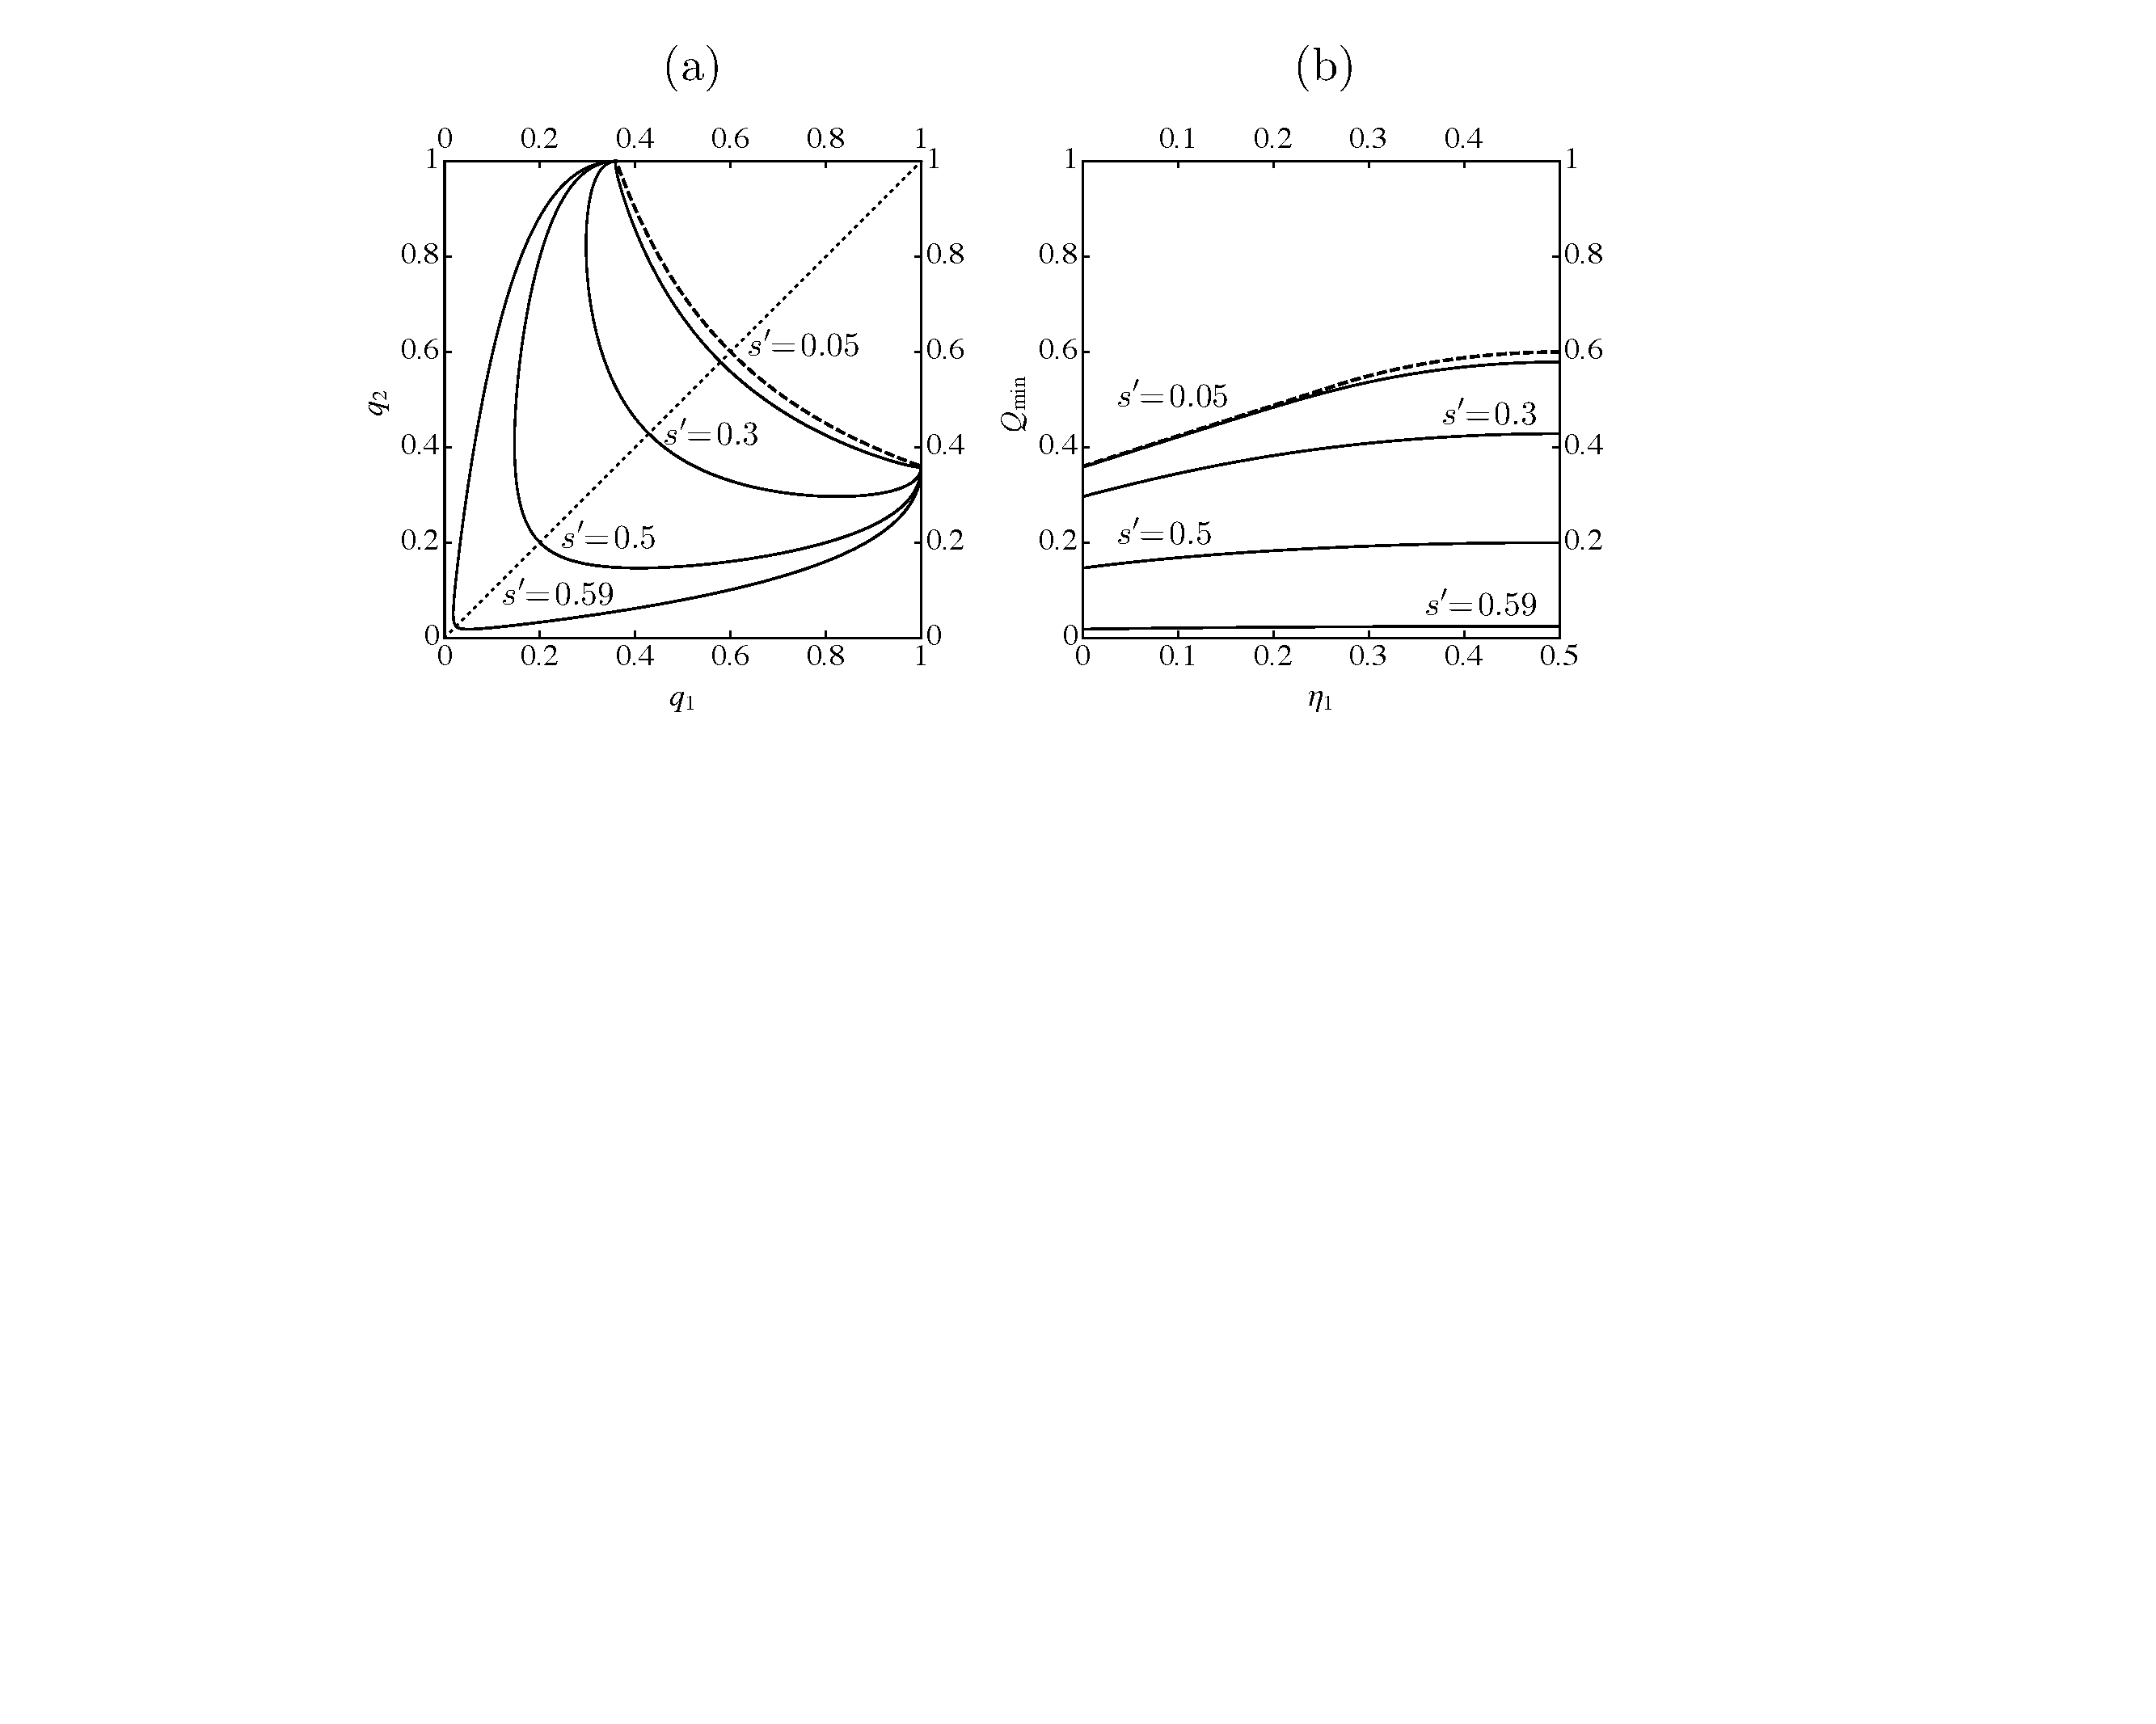
\includegraphics[width=26em]{Separation_F1d.pdf}\\
\end{array}%
$%
\caption{{\color{red}(a) Unitarity curves for different values of~$s'$. The curves are symmetric under mirror reflexion along the  (dotted) straight line $q_1=q_2$, i.e., under the transformation~\mbox{$q_1\leftrightarrow q_2$}.  (b) Minimum separation failure probability~$Q_{\rm min}$ vs. $\eta_1$ (solid lines), for the same values of $s'$ used in~(a). The dashed lines corresponds to full separation/unambiguous discrimination ($s'=0$) in both figures.}}
\label{fig:2}
\end{figure}
%

\section{State Separation: unequal priors }

%%%%%%%%%%%%%%%%%%%%%%%%%%%%%%%%%%%%%%%%%%%%%%%%
%%%%%%%%%%%%%%%%%%%%%%%%%%%%%%%%%%%%%%%%%%%%%%%%

\section{Maximum separation}

In this section, we assume $\eta_1$, $\eta_2$ are fixed given quantities and we focus on the relationship among the initial overlap, the final overlap and the maximum allowed failure rate. To find the explicit form of these relationships, we will need to develop a new geometric view of both the unitarity constraint, Eq.~(\ref{unit cond}), and $Q= \eta_1 q_1+\eta_2 q_2$. %We aim at a simple geometry that would allow both a
We aim at a geometric representation simple enough to grasp visually the solution and yet powerful enough to provide this solution analytically. We show below that the unitary curve and the straight segment of the previous sections can be mapped into conic curves, in particular into families of parabolas and ellipses respectively. This is arguably the simplest extension to our geometric description of state separation. The desired transformation is defined in terms of the new variables $u$ and $v$ as
%
\begin{equation}
u=\sqrt{q_1 q_2};\quad v={q_1+q_2\over 2}.
\label{transf}
\end{equation}
%
They are just the geometric  and arithmetic means of the failure probabilities, $q_1$ and $q_2$. Under this transformation the unitary constraint becomes a parabola that can be conveniently written as
%
\begin{equation}
v={1+u^2\over2}-{(u-s)^2\over2s'^2}.
\label{unit cond conic}
\end{equation}
%
From this expression, one can immediately check that as~$s$ varies we obtain a family of parabolas whose envelope is yet another parabola, $v=(1+u^2)/2$, independently of $s'$. As $s'$ decreases from its maximum value $s'=s$, the parabolas in Eq.~(\ref{unit cond conic}) become thinner. For $s'=0$ they degenerate into the vertical segment $u=s$, $0\le v\le (1+s^2)/2$. These features are illustrated in~Fig.~\ref{fig:3}~(a).

Under the same transformation, {\color{red}Eq.~(\ref{transf})}, the line $Q=\eta_1 q_1+\eta_2 q_2$ becomes an ellipse, which is most easily expressed parametrically in terms of the polar angle $\theta$, measured relative to the axis $v=0$ from the center of the ellipse. It is given by
%
\begin{eqnarray}
u&=&{Q\over\sqrt{1-\Delta^2}}\cos\theta,\nonumber\\
v&=&{Q\over1-\Delta^2}+{Q\Delta\over1-\Delta^2}\sin\theta,
\label{obj fun conic}
\end{eqnarray}
%
where we have defined $\Delta=\eta_2-\eta_1$.  %The semi-major and semi-minor axes can be read of from this equation to be 
It is clear from this expression that the eccentricity of the ellipse is only a function of the priors. For equal priors, $\Delta=0$, the ellipse degenerates into the horizontal segment $v=Q$, $0\le u\le Q$, whereas for $Q=0$ it collapses into the origin $(u,v)=(0,0)$. As one increases $Q$, a family of similar ellipses is obtained. As they increase in size, their center moves up along the axis $u=0$. The line $u=v$ is the envelope of this family, as one can easily check using~Eq.~(\ref{obj fun conic}). Fig.~\ref{fig:3}~(a) also illustrates these features.
%
\begin{figure}[t]
\centering
$%
\begin{array}{c}
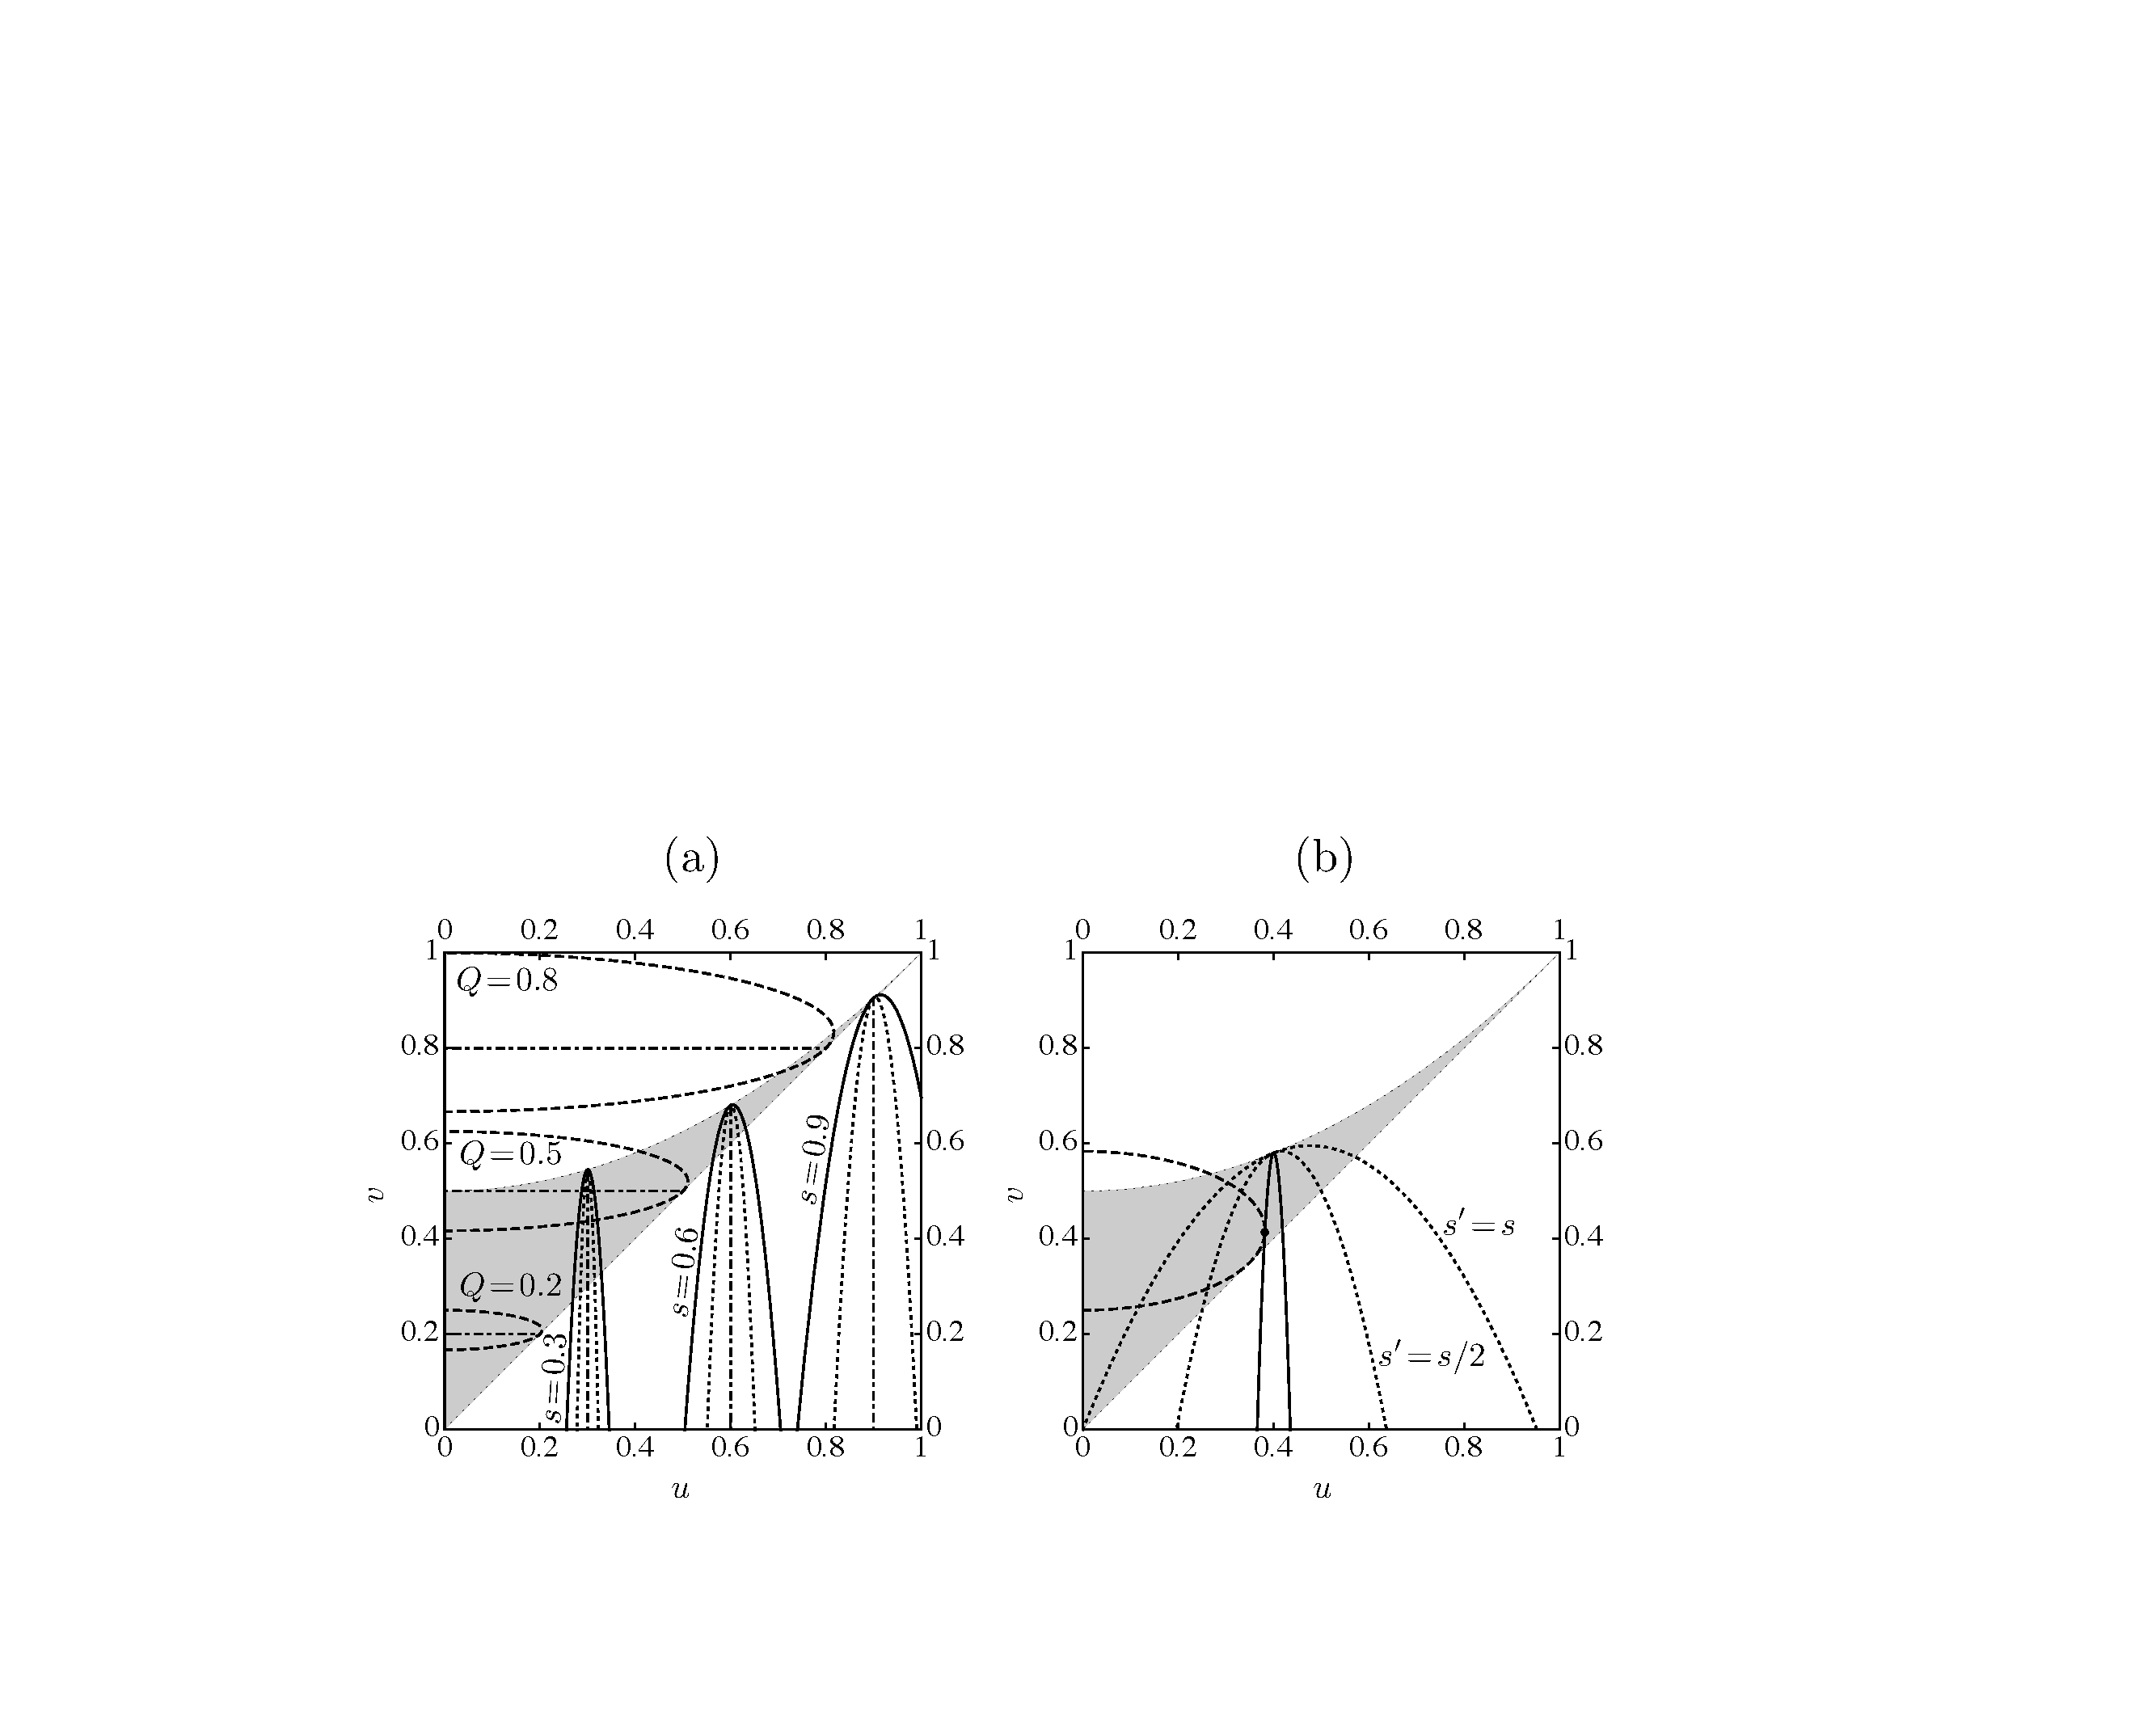
\includegraphics[width=26em]{Separation_F2d.pdf}\\
\end{array}%
$%
\caption{{\color{red}(a) Unitarity parabolas, Eq.~(\ref{unit cond conic}), for different values of~$s$, $s'=s/7$ (solid lines) and $s'=s/14$ (dotted lines). The dashed lines are the ellipses in Eq.~(\ref{obj fun conic}) for various values of the failure rate $Q$. The top boundary line to the gray region, given by $v=(1+u^2)/2$, is the envelope of the solid and dotted parabolas. The bottom boundary line, i.e., the straight line~$v=u$, is the envelope of the family of ellipses (dashed lines). The geometric solution to optimal separation falls in the gray region. In this figure $\eta_1=0.4$. The degenerate curves for $s'=0$ (dot-dashed vertical line) and $\Delta=0$ (dot-dashed horizontal line) are also shown.   (b) Optimal (solid) and suboptimal (dotted) parabolas. The tangency point is also displayed. In this figure $\eta_1=0.3$, $s=0.4$ and $Q=Q_{\rm max}=0.35$. The optimal (minimum) value of $s'$, which gives the solid parabola, turns out to be $s'=0.032$. }}
\label{fig:3}
\end{figure}
%

In terms of this conic geometry,  optimality is again given by a tangency point, this time between ellipses and parabolas. Because of the features of these families of conics, these points of tangency necessarily lie in the region between their envelopes,  which is the gray area in Fig.~\ref{fig:3}. Fig.~\ref{fig:3}~(b) illustrates optimality. Given a maximum failure rate $Q_{\rm max}$ and some initial overlap~$s$ ($Q_{\rm max}=0.35$ and $s=0.4$ in the example considered in the figure), we plot the corresponding ellipse defined by Eq.~(\ref{obj fun conic}) (dashed line). Among the various parabolas, characterized by the final overlap $s'$ (the figure shows two of them, for $s'=s$ and $s'=s/2$), the one that minimizes~$s'$ (solid line) has a unique point of tangency with the ellipse, thus giving us the solution{\color{red}, $s'_{\rm min}$.  To keep the notation simple we will drop the subscript ``$\rm min$'' wherever no confusion arises. }

To find the condition that {\color{red}gives} the tangency point, we first note that {\color{red}the} slopes of the ellipse and the parabolas are given respectively by
%
\begin{eqnarray}
{dv\over du}&=&{v'\over u'}=-{\Delta\over\sqrt{1-\Delta^2}}\cot\theta,\nonumber\\
{dv\over du}&=&u-{u-s\over s'^2},
\label{slopes}
\end{eqnarray}
%
where the prime stands for derivative with respect to the polar angle $\theta$. The right hand side of these two equations must be equal at the tangency point. Moreover, the tangency point must belong to both the ellipse and the optimal parabola. Hence
%
\begin{eqnarray}
Q{1\!+\!\Delta \sin\theta\over 1-\Delta^2}\!&=&\!{1\over2}\!+\!{Q^2\!\cos^2\theta\over2(1\!-\!\Delta^2)}
\!-\!{1\over2 s'^2}\!\!\left(\!{Q\cos\theta\over\sqrt{1\!-\!\Delta^2}}\!-\!s\!\!\right)^{\!\!2}\!\!,\nonumber
%\label{eb21.04.15-1}
\\[.5em]
%
{\Delta\cot\theta\over	\sqrt{1-\Delta^2}}&=&{1-s'^2\over s'^2}{Q\cos\theta\over\sqrt{1-\Delta^2}}-{s\over s'^2}.
\label{eb21.04.15-2}
\end{eqnarray}
%
where to obtain the first (second) equation we have simply substituted Eq.~(\ref{obj fun conic}) into Eq.~(\ref{unit cond conic}) [Eq.~(\ref{slopes})].
Ideally, we would like to solve this system of equations by eliminating $\theta$, which would lead to a closed expression relating~$s$, $s'$ and $Q$. Unfortunately,  this involves solving a high degree polynomial equation in $\cos\theta$. Instead, 
we look at it as a system of two equations with two unknowns, $s$ and $s'$ (or $Q$ and $s'$) and keep $\theta$ as a parameter describing the curve $(s,s')$ [or $(Q,s')$] in parametric form. After some algebra, we obtain the simple expressions:
%
\begin{eqnarray}
s'\!&=&\!- {\sqrt{(1\!-\!Q)^2\!-\!(\Delta\!+\!Q\sin\theta)^2}\over \Delta\!+\!Q\sin\theta}\tan\theta,
\label{eb04.05.15-1}\\[1em]
s\!&=&\!{Q\Delta(1\!+\!\sin^2\theta)\!-\!(1\!-\!\Delta^2\!-\!2Q)\sin\theta\over\sqrt{1\!-\!\Delta^2}(\Delta\!+\!Q\sin\theta)\cos\theta} .
\label{eb04.05.15-2}
\end{eqnarray}
%
The range of values of the parameter $\theta$ in this equation is~$
-\arcsin\Delta\le\theta\le\theta_{\rm max}
$,
where
%
\begin{equation}
\theta_{\rm max}\!=\!\left\{
\!
\begin{array}{lll}
0&\mbox{if}&\displaystyle Q\le 1-\Delta,\\[.7em]
\displaystyle
\arcsin{1-Q-\Delta\over Q}
&\mbox{if}&\displaystyle Q\ge 1-\Delta.
\end{array}
\right.
\label{eb21.04.15-3}
\end{equation}
%
One can easily check the given minimum value of $\theta$ by substituting in Eqs.~(\ref{eb04.05.15-1}) and~(\ref{eb04.05.15-2}) to obtain $s'=s=1$, as it should be. Likewise, one can check that for $\theta=\theta_{\rm max}$ one has $s'=0$.  The two cases in Eq.~(\ref{eb21.04.15-3}) reveal the appearance of the phase transition in the limit $s'\to0$ that we discussed in previous sections. If $Q\ge1-\Delta$, substituting the second line of Eq.~(\ref{eb21.04.15-3}) in Eq.~(\ref{eb21.04.15-2}) we obtain $s=[(2Q+\Delta-1)/(1+\Delta)]^{1/2}$. Solving for $Q$, we find that $Q=\eta_1+s^2\eta_2$. This means that the condition $Q\ge1-\Delta$  is equivalent to $\eta_1+s^2\eta_2\ge 1-\Delta$, which can be immediately seen to give $\eta_1\le s^2/(1+s^2)$. So we obtain the second line in Eq.~(\ref{UD}), corresponding to the ``symmetry-broken phase". If $Q\le 1-\Delta$, namely, if $ s^2/(1+s^2)\le\eta_1$, we have instead $s=Q/\sqrt{1-\Delta^2}$. This equation can be written as $Q=2\sqrt{\eta_1\eta_2}s$. So, Eq.~(\ref{eb21.04.15-3}) has the same content as Eq.~(\ref{UD}). Recall that we are assuming $\eta_1\le1/2\le 1/(1+s^2)$. The third line in Eq.~(\ref{UD}) never applies under this assumption.

\begin{figure}[t] %  figure placement: here, top, bottom, or page
   \centering
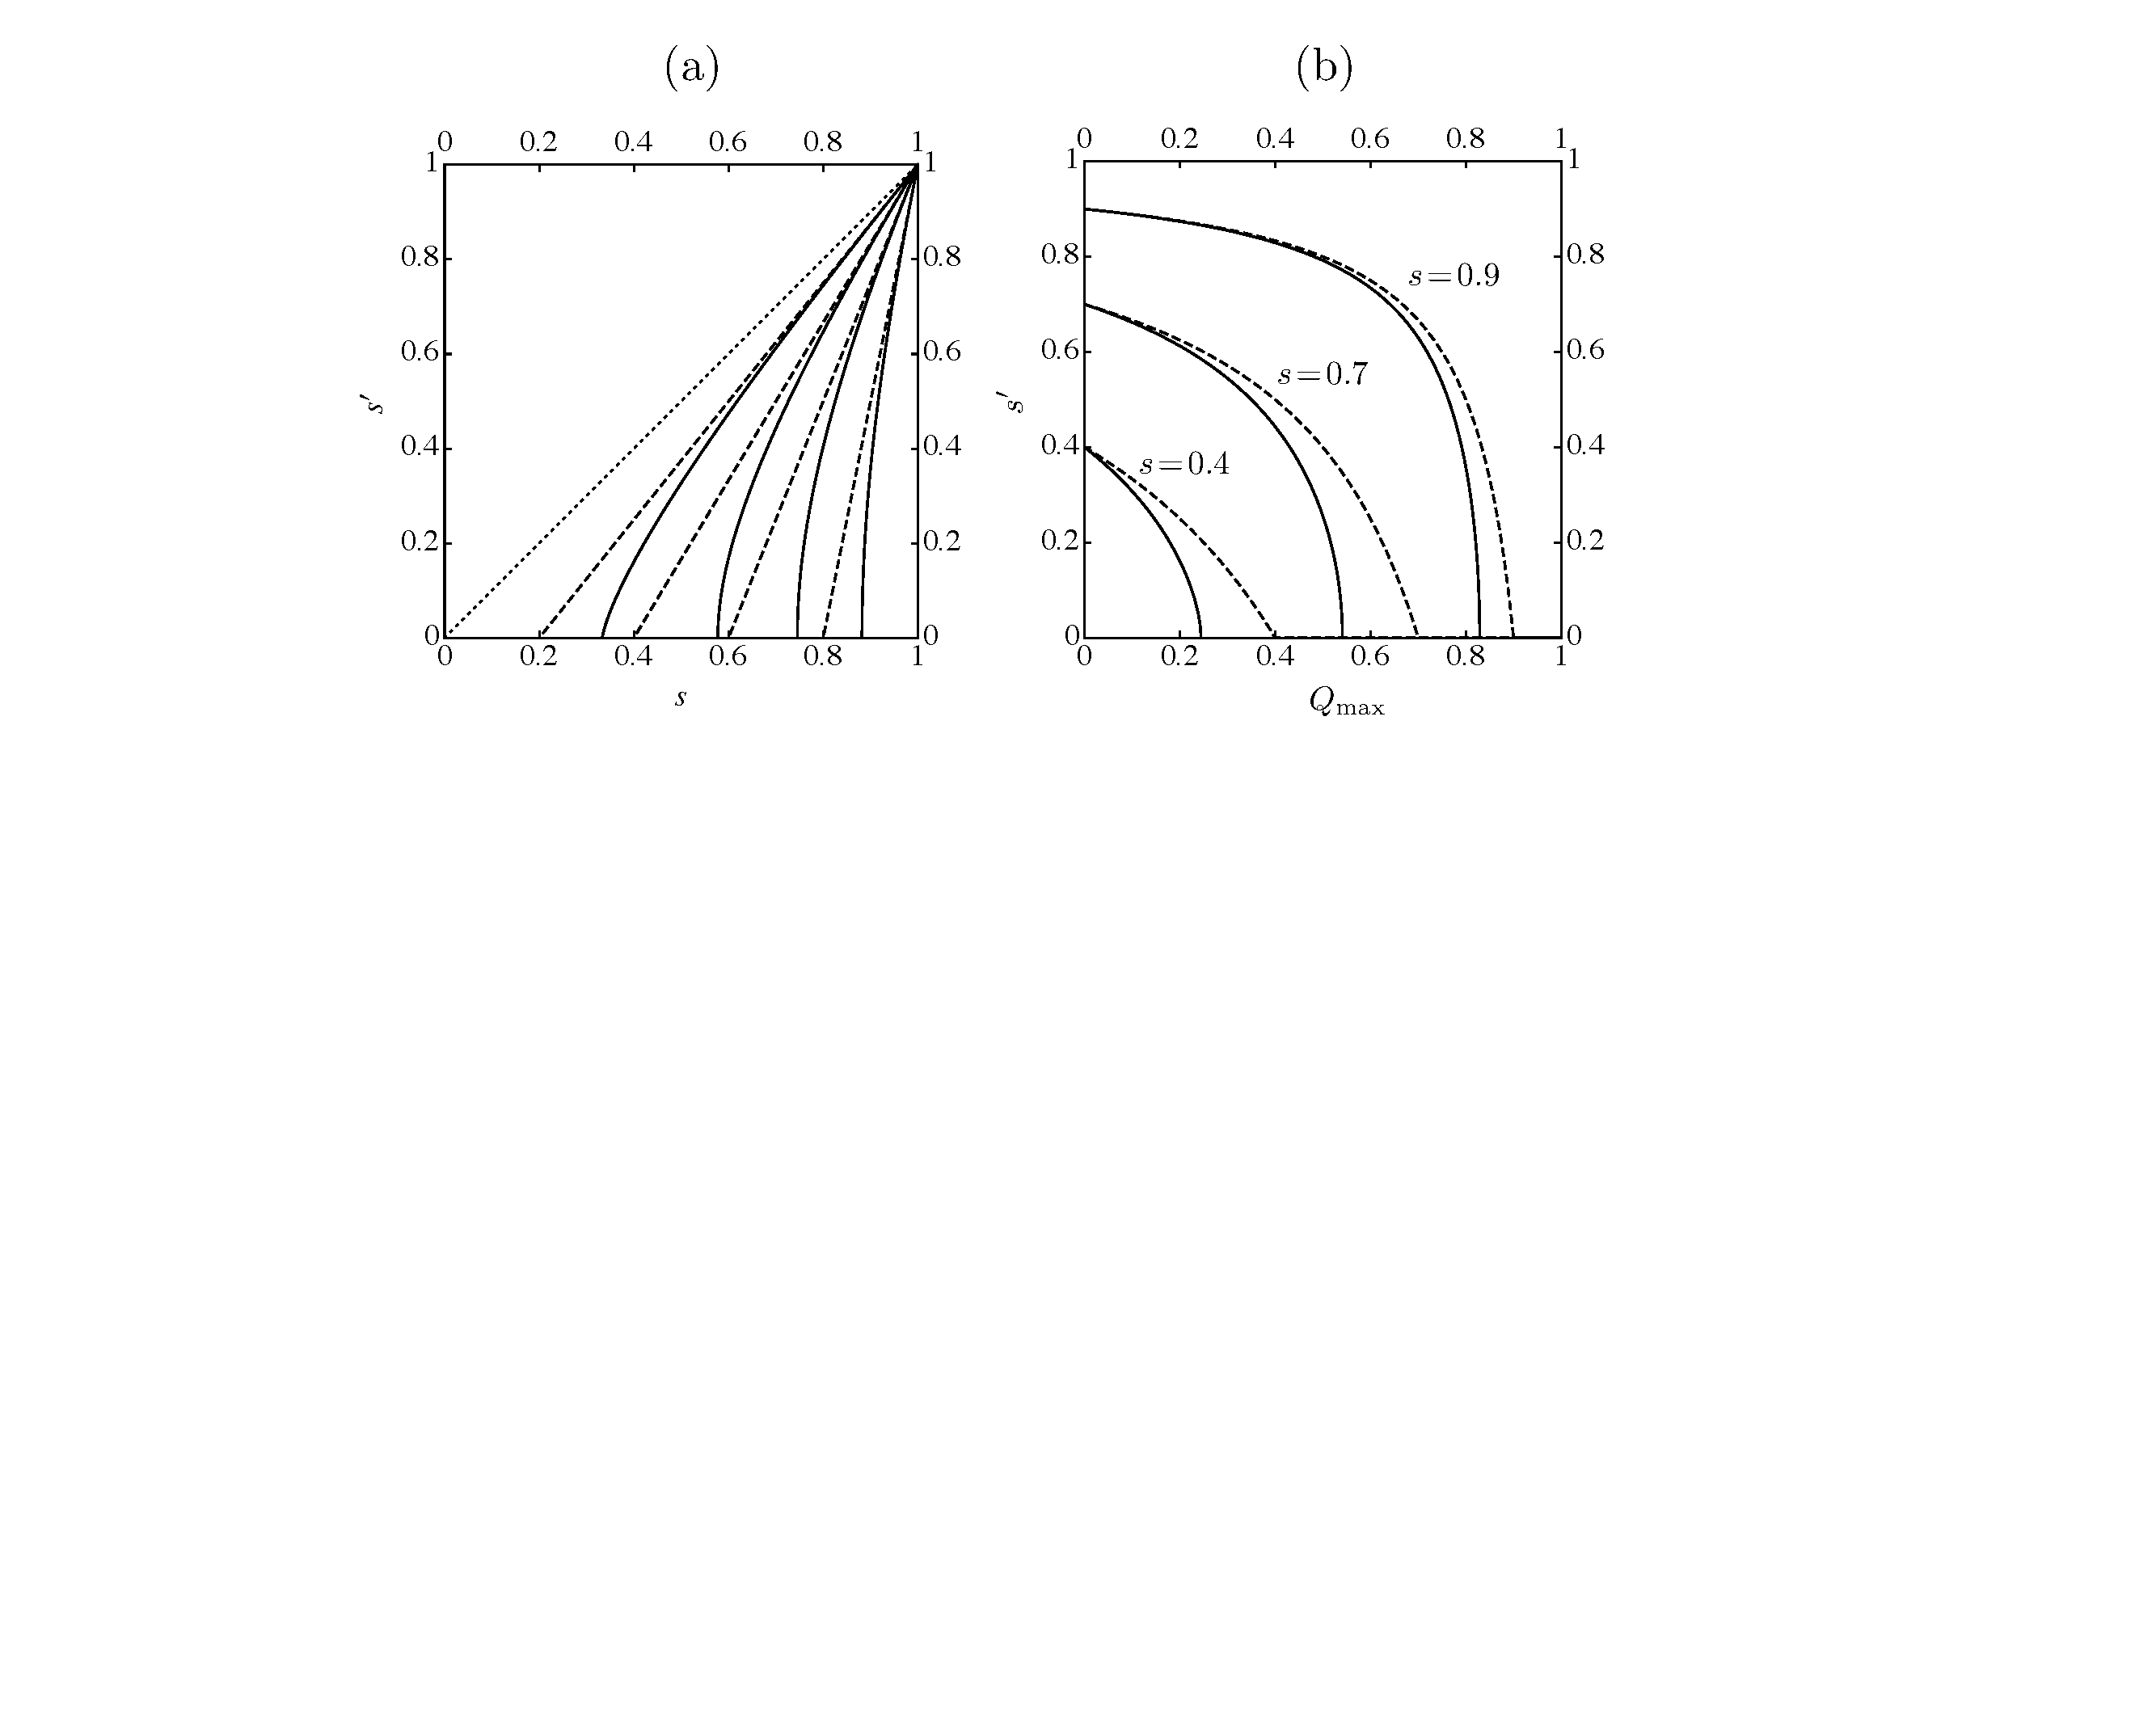
\includegraphics[width=26em]{Separation_F3_4}
   \caption{(a) Plots of $s'$ vs. $s$ for $\eta_1=0.1$ (solid lines) and $\eta_1=0.5$ (straight dashed lines) and for values of the failure rate. From left to right $Q_{\rm max}=0.2$, $0.4$, $0.6$, $0.8$. The dotted line is the (trivial) curve for $Q_{\rm max}=0$, which is the straight line $s'=s$. (b)~Minimum final overlap vs. maximum failure probability for various values of the initial overlap and the same two values of $\eta_1$ used in~(a).\vspace{-1em}
   }
   \label{fig:4}
\end{figure}

Eqs.~(\ref{eb04.05.15-1}) and~(\ref{eb04.05.15-2}) are plotted in Fig.~\ref{fig:4}~(a) for two possible priors: $\eta_1=0.1$ (solid lines) and $\eta_1=0.5$, i.e., for equal priors  (dashed lines). From left to right, the maximum allowed failure rate~$Q_{\rm max}$ is $0.2$, $0.4$, $0.6$ and~$0.8$. We see that for small values of the initial overlap, $s$, one can attain full separation ($s'=0$). Past the critical value,
%%
%\begin{equation}
%s_{\rm cr}=
%\left\{
%\begin{array}{lll}
%\displaystyle {Q_{\rm max}\over\sqrt{1-\Delta^2}}={Q_{\rm max}\over 2\sqrt{\eta_1\eta_2}}&\mbox{if}&\displaystyle Q\le 1-\Delta,\\[1em]
%\displaystyle
%\sqrt{2Q_{\rm max}+\Delta-1\over1+\Delta}
%&\mbox{if}&\displaystyle Q\ge 1-\Delta,
%\end{array}
%\right.
%\end{equation}
%%
%
\begin{equation}
s_{\rm cr}=
\left\{
\begin{array}{lll}
\displaystyle{Q_{\rm max}\over 2\sqrt{\eta_1\eta_2}}&\mbox{if}&\displaystyle Q\le 2\eta_1,\\[1.2em]
\displaystyle
\sqrt{Q_{\rm max}-\eta_1\over\eta_2}
&\mbox{if}&\displaystyle Q\ge 2\eta_1,
\end{array}
\right.
\end{equation}
%
 full separation is no longer possible and~$s'$ increases (quite abruptly for small $\eta_1$). In the region $s<s_{\rm cr}$, the margin $Q_{\rm max}$ is not necessarily saturated,  since the unambiguous discrimination failure probability $Q_{\rm UD}$ is  smaller than $Q_{\rm max}$. For $s\ge s_{\rm cr}$ we necessarily have to saturate the margin, $Q=Q_{\rm max}$. For equal priors (dashed lines) one can obtain the curves in explicit form from Eq.~(\ref{unit cond}) using that $q_1=q_2=Q$:
%
\begin{equation}
s'=
\left\{
\begin{array}{lll}
\displaystyle0 &\mbox{if}& s\le Q_{\rm max},\\[.7em]
\displaystyle
{s-Q_{\rm max}\over 1-Q_{\rm max}}
&\mbox{if}&\displaystyle s\ge Q_{\rm max}.
\end{array}
\right.
\label{tradeoff equal}
\end{equation}
% 
This expression could also be obtained by carefully taking the limit $\Delta\to 0$ in Eqs.~(\ref{eb04.05.15-1})  through~(\ref{eb21.04.15-3}).
The figure clearly shows that separation becomes less demanding as we move away from the equal prior case. For \mbox{$Q_{\rm max}=0$}, i.e., in the deterministic limit, we recover the trivial solution $s'=s$ (dotted line).

\vspace{10em}

\section{Tradeoff between Maximum separation and failure rate}

By solving the system Eq.~(\ref{eb21.04.15-2}) for $Q$ and $s'$ , we obtain a parametric expression for the tradeoff curve $(Q,s')$ in terms of the polar angle $\theta$:
%
%\begin{widetext}
%%%
%%\begin{eqnarray}
%%s'^2&=&\sqrt{1-\Delta^2}\,{\sqrt{1-\Delta^2}(1+s^2)\cos\theta-2s\left(1+\Delta \sin\theta\right)\over(\Delta+\sin\theta)^2} {\sin^2\theta\sec\theta},\label{eb29.04.15-1}\\[.5em]
%%%
%%Q&=&{s\sqrt{1-\Delta^2}+\Delta\,s'^2\cot\theta\over(1-s'^2)\cos\theta}.
%%\label{eb29.04.15-2}
%%\end{eqnarray}
%%%
%%
%\begin{equation}
%s'^2=\sqrt{1-\Delta^2}\left({\sin\theta\over\Delta+\sin\theta}\right)^2{\sqrt{1-\Delta^2}(1+s^2)\cos\theta-2s\left(1+\Delta \sin\theta\right)\over\cos\theta} ;\qquad
%%
%Q={s\sqrt{1-\Delta^2}+\Delta\,s'^2\cot\theta\over(1-s'^2)\cos\theta}.
%\label{tradeoff}
%\end{equation}
%%
%\end{widetext}
%
%
\begin{eqnarray}
s'^2\!&=&\!\sqrt{1\!-\!\Delta^2}\left({\sin\theta\over\Delta\!+\!\sin\theta}\right)^2\nonumber
\\
\!&\times&\!{\sqrt{1\!-\!\Delta^2}(1\!+\!s^2)\!\cos\theta\!-\!2s\!\left(1\!+\!\Delta \sin\theta\right)\over\cos\theta} ,
\label{tradeoff1}\\[.5em]
%
Q&=&\!{s\sqrt{1\!-\!\Delta^2}\!+\!\Delta\,s'^2\!\cot\theta\over(1\!-\!s'^2)\cos\theta}.
\label{tradeoff2}
\end{eqnarray}
%
Note that Eq.~(\ref{tradeoff1}) is an expression for the square of the final overlap. To keep the formula for~$Q$, Eq.~(\ref{tradeoff2}), %, for $Q$, 
short, we use~$s'^2$ as a shorthand for Eq.~(\ref{tradeoff1}).  %in the formula for $Q$ in Eq.~(\ref{tradeoff}). It is understood that one has to substitute the first formula for $s'$. 
%
The range of $\theta$ in Eqs.~(\ref{tradeoff1}) and~(\ref{tradeoff2}) is:
$$
-\arctan\,{s\Delta\over\sqrt{1-\Delta^2}}\le\theta\le\theta_{\rm max},
$$
where the upper limit  of the interval can be written as
%
\begin{equation}
\theta_{\rm max}\!=\!\left\{
\!
\begin{array}{lll}
0&\mbox{if}&\displaystyle \eta_1\!\ge\!{s^2\over1\!+\!s^2},\\[1em]
\displaystyle \!-\!\arccos\!{2s\sqrt{1-\Delta^2}\over1\!-\!\Delta\!+\!s^2(1\!+\!\Delta)}
&\mbox{if}&\displaystyle \eta_1\!\le\!{s^2\over1\!+\!s^2}.
\end{array}
\right.
\label{tradeoff cases}
\end{equation}
%
The lower limit  in the range of allowed $\theta$  can be derived from Eqs.~(\ref{tradeoff1}) and~(\ref{tradeoff2}) by imposing that $Q=0$ at $s'=s$. The upper limit can be derived from Eq.~(\ref{tradeoff1}) by imposing $s'=0$. Once again, we see that a second order phase transition occurs in the limit of full separation: by substituting the first (second) line of Eq.~(\ref{tradeoff cases}) in Eq.~(\ref{tradeoff2}) we obtain $Q=s\sqrt{1-\Delta^2}$\ ($Q=[1-\Delta+s^2(1+\Delta)]/2$), which is the first (second) case in Eq.~(\ref{UD}).

Fig.~\ref{fig:4}~(b) shows various plots of the separation vs. failure-rate tradeoff curve. As in Fig.~\ref{fig:3}, the plots are for~$\eta_1=0.1$ (solid lines) and for equal priors, $\eta_1=\eta_2=0.5$ (dashed lines). For equal priors, there is the explicit formula for the curves given in Eq.~(\ref{tradeoff equal}). Again, we see that as $\eta_1$ gets smaller, departing from the equal prior value~$1/2$, the states can be separated more for the same maximum rate of failure. As $Q_{\rm max}$ increases, the minimum overlap gets smaller, as it should. When~the margin~$Q_{\rm max}$ reaches the unambiguous discrimination value~$Q_{\rm UD}$ we have $s'=0$, attaining full separation. Larger values of~$Q_{\rm max}$ are rather meaningless in this context, since they will never be saturated by an optimal protocol, which requires  a failure rate of only $Q=Q_{\rm UD}$~($<Q_{\rm max}$) to fully separate the input states.

%%%%%%%%%%%%%%%%%%%%%%%%%%%%%%%%%%%%%%%%%%%%%%%%
%%%%%%%%%%%%%%%%%%%%%%%%%%%%%%%%%%%%%%%%%%%%%%%%
\chapter{Linear Optical Experimental Realizations}
\section{Implementation of Pure State Interpolative Discrimination}

Our experimental implementation is similar to the one derived for Unambiguous Discrimination by Bergou, Hillery and Sun \cite{Bergou}. We derive first the implementation of the intermediate scheme for pure states with equal a-priori probabilities, then we obtain the general result.  We use a six-port and the 'rail representation' of optical axes;  three input ports, or rails, and three output ports each represent a degree of freedom.  In this two-step measurement process the first step produces the failure rate or makes the input state more distinguishable.  The second step measures the state if the first step did not produce a failure result.  Our Hilbert space differs from the previous section in that we use a direct sum to add a single degree of freedom to the qubit space, instead of a tensor product ancilla.

\section{First Measurement}
For the first step, our equations are:

\[U \ke {\psi_1}= \sqrt{p_1} \ke {\phi_1} + \sqrt{q_1} \ke 3\]
\[U \ke {\psi_2}= \sqrt{p_2} \ke {\phi_2}  + \sqrt{q_2} \ke 3\] 

Here the 'ancilla' , $ \ke 3$, is the empty portion of the input state $\ke {\psi_i} = \alpha \ke 1 + \beta \ke 2 + 0 \ke 3$, and if it remains empty  then we have successfully transformed the input state into a more orthogonal state where we define $ \bk {\phi_1} {\phi_2} = \gamma$ as the overlap of the output states..  However if it becomes occupied then the measurement failed. 

For our implementation scheme we consider the input states

\[ \ke {\psi_1} = cos \theta \ke 1 + sin \theta \ke 2\]
\[ \ke {\psi_2} = \ke 1\]


The output of the six-port for $\ke {\psi_1}$ is

\[\ke {out_1} = \sum^3 (cos\theta  U_{j1}  + sin \theta U_{j2}) \ke j\]
and for $\ke {\psi_2}$ is
\[\ke {out_2} = \sum^3 ( U_{j1}) \ke j\]


where the U matrix represents the action of the Unitary operator acting on the system.
If we measure output three we get the failure as

\[q = \vert \alpha U_{31} + \beta U_{32} \vert ^2\] 
This depends on the input state.

The outputs of the other two rails are

\[ \ke {\phi_1} = \]
\[ (U_{11} cos \theta + U_{12} sin \theta) \ke 1 + (U_{21} cos\theta + U_{22} sin \theta)\ke 2\]

\[ \ke {\phi_2} = U_{11} \ke 1 + U_{21} \ke 2\]

For UD we wanted the output states to be orthogonal.  For the general IM scheme we want to vary the overlap of the output states, so we call the output overlap $ \bk {\phi_1} {\phi_2} = \gamma$ 

This is also a condition on U:

\[(1- \abs U_{31}^2) cos\theta - U_{31}^* U_{32} sin \theta = \gamma\]

The failure probabilites for the states are:

\[q_1 = \abs {U_{31} cos \theta + U_{32} sin \theta}^2\]
\[q_2 = \abs  U_{31}^2\]

Now their product is

\[q_1 q_2 =   \abs { \abs U_{31}^2 cos \theta + U_{31}1^*  U_{32} sin \theta}^2 = \abs { cos\theta - \gamma}^2\]

Where we used the $\gamma$ identity above.
\subsection{Equal A-priori Probabilities}
The first solution we attempt is for equal priors $\eta_1 = \eta_2$ where we know the optimal solution is $q_1 = q_2 = cos\theta - \gamma$ since we can assume $cos \theta > \gamma$

We can now determine the first two matrix elements from the preceding equations. Immediately 

\[U_{31} = (cos\theta - \gamma)^{1/2}\]
From $q_1$ and from $ q_2$ we get
\[U_{32} = \frac{(cos \theta - \gamma)^{1/2}[1-cos\theta]}{sin\theta} =  (cos \theta - \gamma)^{1/2} tan \frac{\theta}{2}\]
Using $ sin \theta = [(1+cos \theta)(1-cos \theta)]^{1/2}$ and $\tan \frac{\theta}{2} = (\frac{1-cos \theta}{1+cos \theta})^{1/2}$

From the unitary requirement of U we know $\abs {U_{31}}^2 + \abs {U_{32}}^2 + \abs {U_{33}}^2 = 1$ so we find 

\[\abs {U_{33}}^2  = \frac{1- cos \theta + 2 \gamma}{1+cos \theta}\]

This is where our solution departs from the original paper.  The reason is that the assumption of the same two beam splitters doesn't work, so we start with the general formalism of decomposing a 3x3 matrix with real elements into 3 beam splitters.

The diagramatic approach to the 3 rail representation is shown below.


\begin{figure}[th]
\centering
$%
\begin{array}{c}
\includegraphics[height=4 cm]{ud.jpg} \\ 
 
\end{array}
$%
\end{figure}

We see that at each interseciton of rails, of which there are 3, a beam splitter is necessary.  We call the three beam splitters M1, M2 and M3 such that $U = M3*M2*M1$ and

\[ M1= \begin{pmatrix} 
1 & 0 & 0\\
0 &x1 & -x2\\
0&x2 & x1\\
\end{pmatrix}\]

\[ M2= \begin{pmatrix} 
y1&0&-y2\\
0&1&0\\
y2&0&y1\\
\end{pmatrix}\]

\[ M3= \begin{pmatrix} 
z1&-z2&0\\
z2&z1&0\\
0&0&1\\
\end{pmatrix}\]

This gives us the general expression for U to be

\[ U= \begin{pmatrix} 
z1y1&-z1y2x2+z2x1&z1y2x1+z2x2\\
-z2y1&z2y2x2+z1x1&-z2y2x1+z1x2\\
-y2&-y1x2&y1x1\\
\end{pmatrix}\]

Where we can use the property of reflection/transmittion coefficients of beam splitters to simplify them as: $x1^2 + x2^2 =1$, $y1^2+y2^2=1$, $z1^2+z2^2 =1$

Since we have the terms for the last row of M, we can solve for x1 and y1 to find

\[x1 = [\frac{1-cos \theta +\gamma - (cos \theta -\gamma)tan ^2 \frac{\theta}{2}}{1-cos \theta + \gamma}]^{1/2}\]
\[y1 = (1-cos \theta + \gamma)^{1/2}\]

Now only the z values are undetermined and curiously, the unitarity of M does not depend on the z values hence we can conclude that the M3 beam splitter is unnecessary, and leave it as the identity. 

This concludes the equal priors case.
\subsection{General A-priori Probabilities}
For the general case we have to consider $\eta_1 q_1 + \eta_2 q_2 = Q$ as the equation from which we draw our solutions.   There exists a single-state domain region where the POVM solution does not hold but we will not discuss it here. The optimal solution otherwise, as was derived in the previous section of the paper, was shown to be $\eta_1 q_1 = \eta_2 q_2$.  . We can apply this constraint to the problem to solve for each $q_i$ separately:

\[\frac{\eta_1}{\eta_2} q_1^2 = \frac{\eta_2}{\eta_1} q_2^2= (cos \theta - \gamma)^2\]

hence

\[q_1 = \sqrt{  \frac{\eta_2}{\eta_1} } (cos \theta -\gamma)\]

\[q_2 =\sqrt{\frac{\eta_1}{\eta_2}  } (cos \theta -\gamma)\]

It is interesting that we can simply find the relation between the fixed failure rate of the problem and the overlap of the output states:

\[Q = 2 \sqrt{\eta_1 \eta_2} (cos \theta - \gamma)\]

This correctly meets both bounds: at $\gamma = 0$ we have $Q = Q_0$ and we have attained the UD bound for failure rate.  At $\gamma = cos \theta$ we have the ME limit where $Q = 0$.

We continue with our solution to find the first matrix elements:

\[ U_{31} = \delta (cos \theta - \gamma)^{1/2}\]

\[U_{32} = \frac{(cos \theta - \gamma)^{1/2} (1 - \delta^2 cos \theta)}{\delta sin \theta}\]

where $\delta = (\frac{\eta_1}{ \eta_2})^{1/4}$

We can again solve for the x1 and y1 terms:

\[x1 = [\frac{\delta^2 sin^2 \theta - (cos \theta -\gamma)[\delta ^4 -2 \delta^2 cos \theta +1]}{\delta^2 sin^2 \theta(1-\delta^2(cos \theta -\gamma))}]^{1/2}\]
\[y1 = (1-\delta^2(cos\theta -\gamma))^{1/2}\]

Interestingly, agian the z terms are unimportant so the general solution needs only two beam splitters.
\subsection{Second Measurement}
The second measurement is a minimum error strategy that discriminates optimally between the two input states.  We use the same method as for the first measurement, except with only two rails.

Our input states are $\ke {\phi_1} = \alpha_1 \ke 1 + \beta_2 \ke 2$ and $\ke {\phi_2} = \alpha_2 \ke 1 + \beta_2 \ke 2$ where we've kept the coefficients arbitrary for now.The output states are $\ke {\xi_1}$ and $\ke {\xi_2} $ respectively.

The effect of the unitary is

\[U\ke {\phi_1} = \sqrt{p_1} \ke 1 + \sqrt{r_1} \ke 2\]
\[U \ke {\phi_2} = \sqrt{p_2} \ke 2 + \sqrt{r_2} \ke 1\]

and the output states  are

\[ \ke {\xi_1} = \]
\[ (U_{11} \alpha_1 + U_{12}\beta_1) \ke 1 + (U_{21} \alpha_1 + U_{22}\beta_1)\ke 2\]
\[ \ke {\xi_2} = \]
\[ (U_{11} \alpha_2 + U_{12}\beta_2) \ke 1 + (U_{21} \alpha_2 + U_{22}\beta_2)\ke 2\]

the error rates are associated with detector 1 clicking for state $\phi_2$ and detector 2 clicking for state $\phi_1$, hence

\[r_1 =  (U_{21} \alpha_1 + U_{22}\beta_1)\]
\[r_2 =  (U_{11} \alpha_2 + U_{12}\beta_2)\]

\subsubsection{Example}

For completeness' sake we present an example of the previous implementation.  We plot the x1 and y1 coefficients vs $\gamma$ for $cos \theta = \pi /4 $ and $\eta_1 = 3/5$.   We can see from Fig. 1 that the M1 beam splitter remains very nearly the identity for all ranges of output angles.  The main effect is in fact in the work of the M2 BS.

%%%%%%%%%%%%%%%%%%2D GRAPHS

%%%%%%%%%%%%%%%%%%%%%%%%%%%%%%%%% 3D GRAPHS

  To fully exhibit the relationship between the initial overlap, final overlap and beam splitter coefficients we include Fig. 3 and 4, where the limited functionality of M1 is fully visible.  These plots are for the POVM region, which must satisfy the condition \cite{Bagan}

\[\frac{cos^2 \theta}{1+ cos^2 \theta} \leq \eta_1 \leq \frac{1}{1+cos^2\theta}\]



%%%%%%%%%%%%%%%%%%%%%%%%%%%%%%%%%%%%%%%%%%%%%%%%
%%%%%%%%%%%%%%%%%%%%%%%%%%%%%%%%%%%%%%%%%%%%%%%%
\section{Implementation of State Separation }

In this chapter we propose a straightforward proof-of-principle implementation of {\color{red}optimal} separation, sketched in Fig.~\ref{fig:5}. The implementation uses only %the straightforward 
linear optics elements, namely, a mirror and two beam splitters, BS1 and~BS2. The measurement are carried out  by three photodetectors. %The setup is sketched in Fig.~\ref{fig:5}. 
The three income ports, labeled \mbox{$1$, $2$, $3$} in the figure, are in a superposition of zero and/or one photons, corresponding to the orthogonal states~$|0\rangle$, i.e., the vacuum state, $|1\rangle=a_1^\dagger|0\rangle$,  $|2\rangle=a_2^\dagger|0\rangle$ and $|3\rangle=a_3^\dagger|0\rangle$, where~$a_i^\dagger$ is the creation operator of the electromagnetic field in port~$i$, $i=1,2,3$. Similarly, for the output ports we have~$|1'\rangle=a_1'{}^\dagger|0\rangle$,  $|2'\rangle=a_2'{}^\dagger|0\rangle$ and $|3'\rangle=a_3'{}^\dagger|0\rangle$.

In terms of these basis states, Eqs.~(\ref{U1}) and~(\ref{U2}) can be written as
\begin{eqnarray}
U |1\rangle&=&\sqrt{p_1}|1'\rangle+\sqrt{q_1}|3'\rangle,\label{U1 impl}\\[.2em]
U\left( s|1\rangle+\sqrt{1-s^2} |2\rangle\right)&=&\sqrt{p_1}\left( s'|1'\rangle+\sqrt{1-s'^2} |2'\rangle\right)+\sqrt{q_1}|3'\rangle,\label{U2 impl}
\end{eqnarray}

%
which corresponds to the choice: $|\psi_1\rangle|0\rangle=|1\rangle$, $|\psi_2\rangle|0\rangle=s|1\rangle+\sqrt{1-s^2}|2\rangle$, $|\psi'_1\rangle|\alpha_1\rangle=|1'\rangle$, $|\psi'_2\rangle|\alpha_2\rangle=s'|1'\rangle+\sqrt{1-s'^2}|2'\rangle$ and $|\phi\rangle|\alpha_0\rangle=|3'\rangle$. So, input port $3$ is always in the vacuum state. The detection of a photon in the output port $3'$ signals that separation failed. The state~$|\psi_2\rangle$ can be produced  in a standard way by sending a photon into a beam splitter with suitable transmission and reflection coefficients.
%
\begin{figure}[h] %  figure placement: here, top, bottom, or page
   \centering
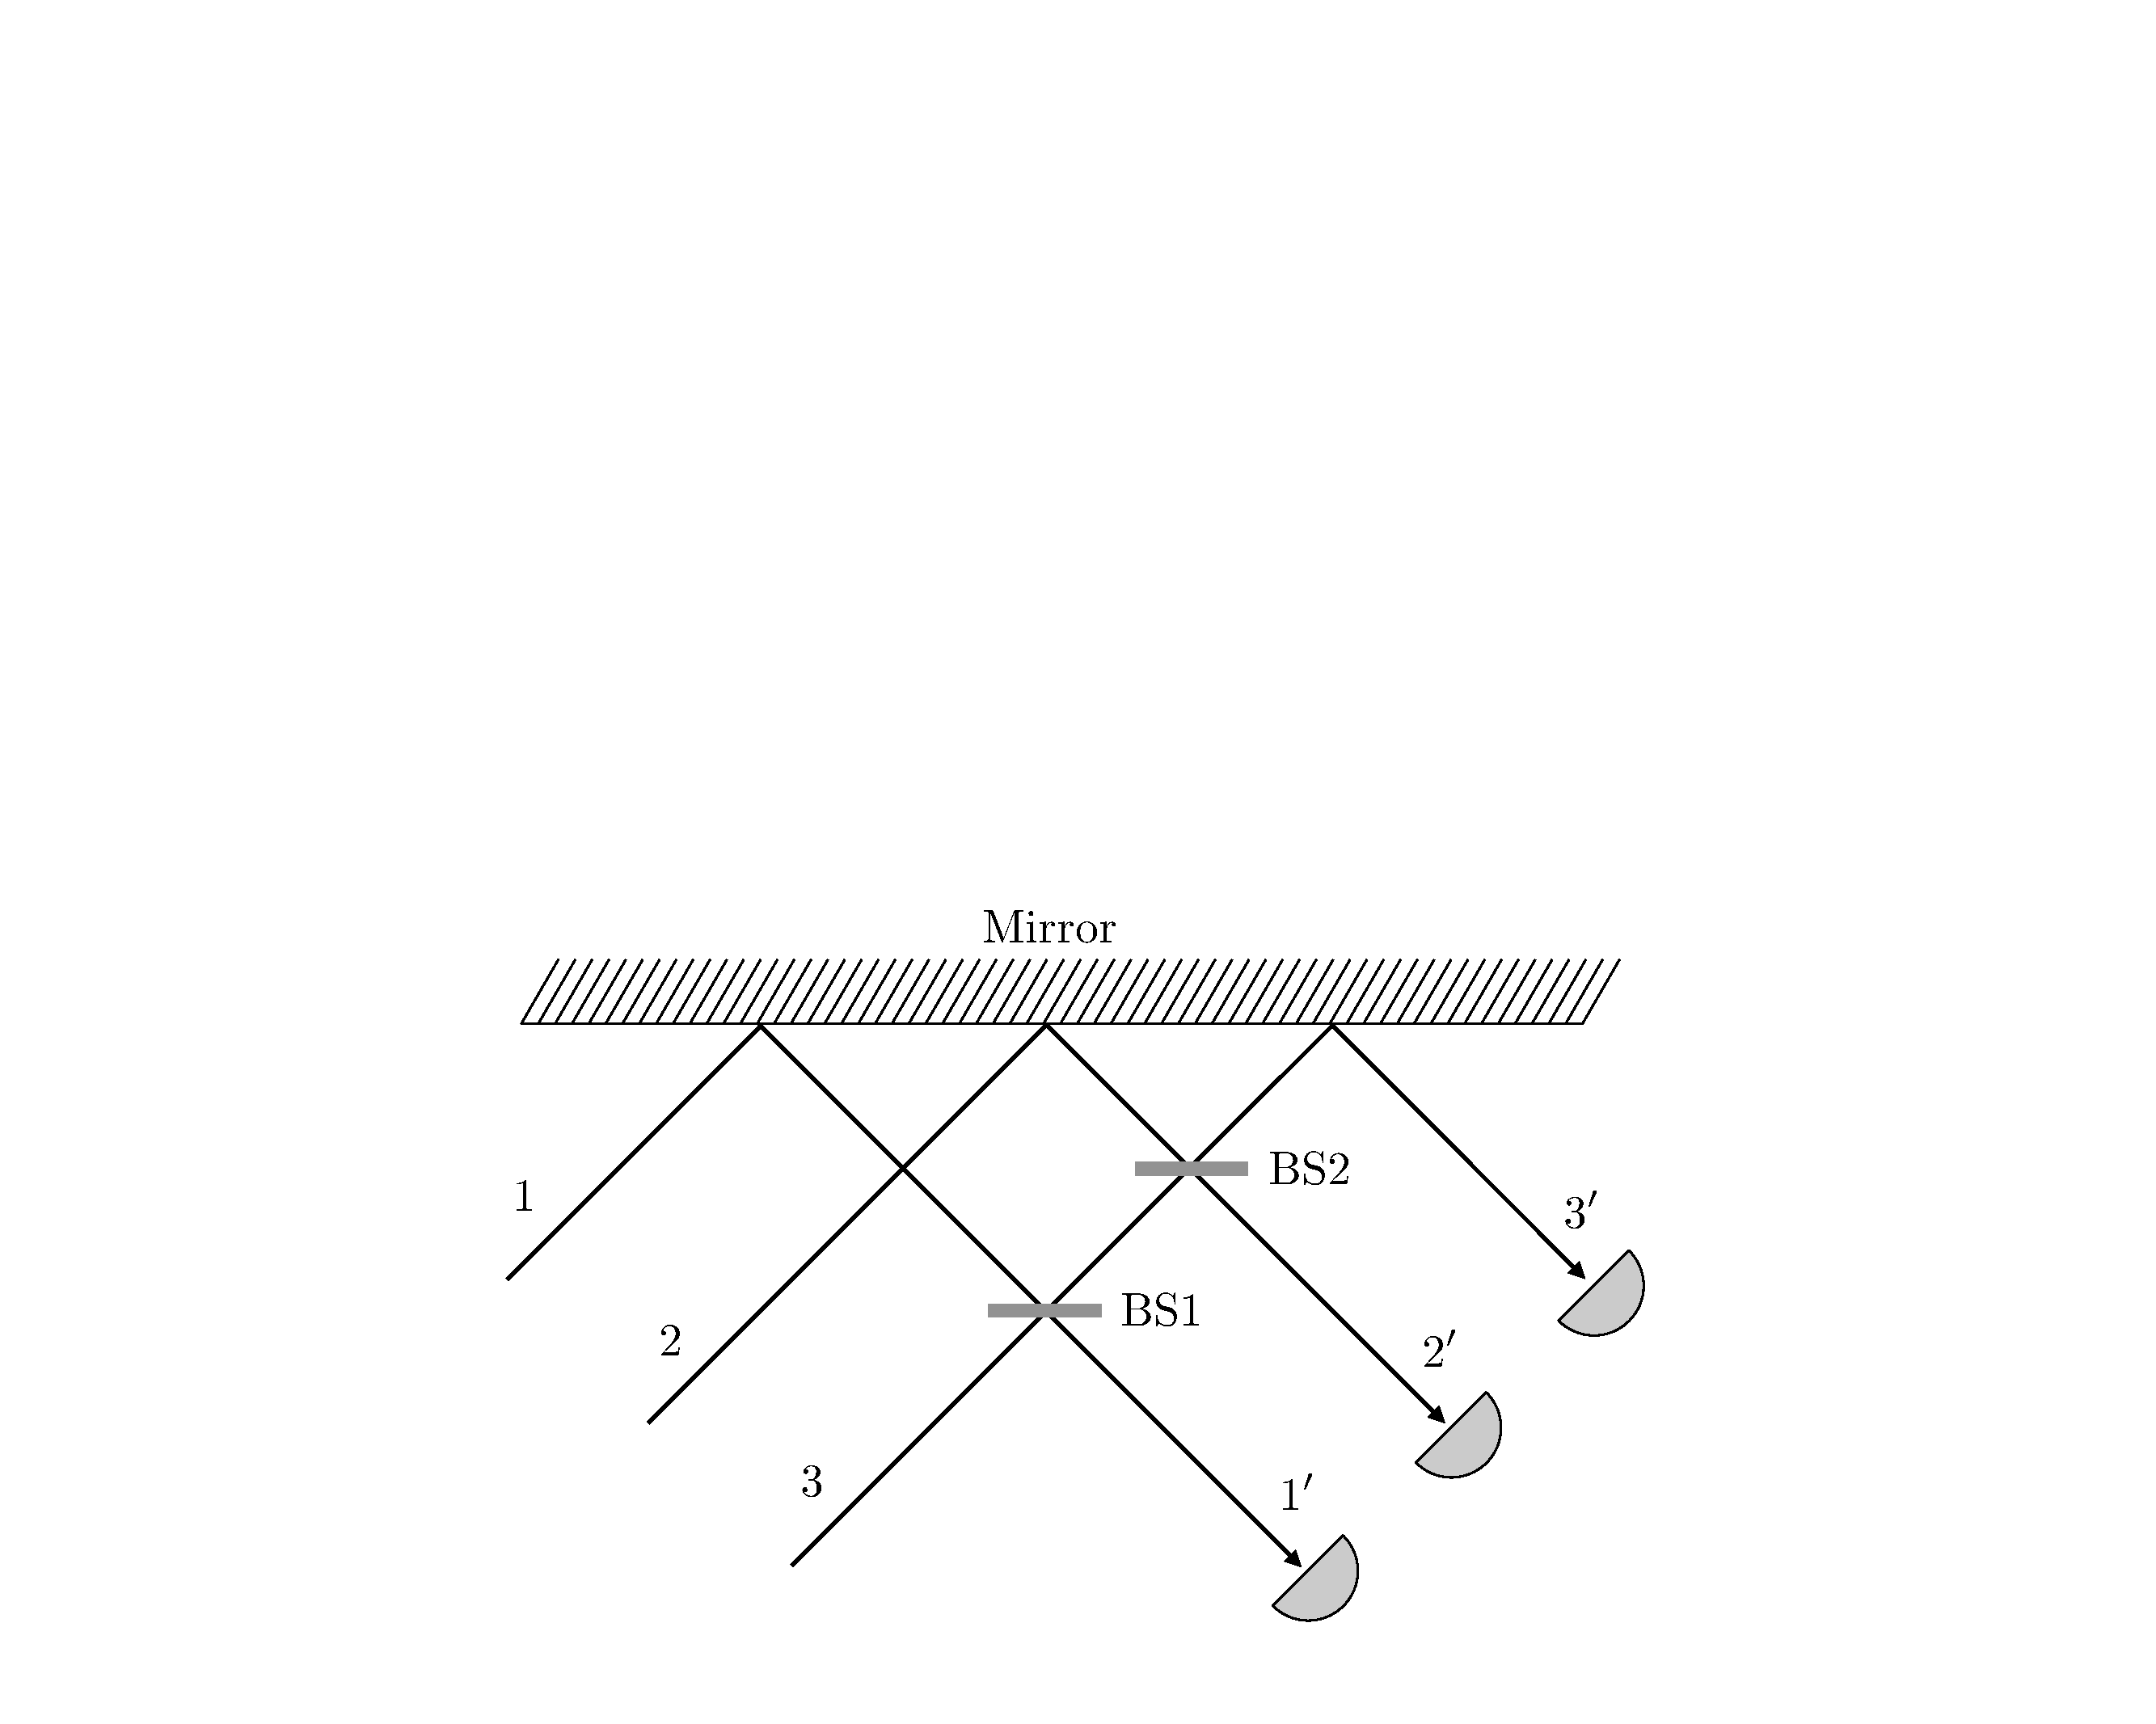
\includegraphics[width=18em]{Separation_F5}\vspace{2em}
   \caption{Six-port linear optics implementation of a proof-of-principle separation protocol. The transmission (reflexion) coefficients of the beamsplitters, BS1 and BS2 are given by the (off-)diagonal entries of the matrices in Eqs.~(\ref{M1}) and~(\ref{M2}), respectively. The input states are feed through ports $1$ and $2$ as a superposition of zero and one photons in each port. The separated states are output through ports $1'$ and $2'$. Port $3$ is in the vacuum state. A click in the photodetector placed in port $3'$ signals failure.}
   \label{fig:5}
\end{figure}
%

For simplicity, we consider equal prior probabilities $\eta_1=\eta_2=1/2$, but the same setup can be used in the general case. As mentioned above, for equal priors we must have $q_1=q_2=Q$ and $p_1=p_2=1-Q$ and the unitarity condition Eq.~(\ref{unit cond}) can be solved explicitly. The solution is given by $Q=Q_{-1}$ in Eq.~(\ref{Q's}). Substituting in Eqs.~(\ref{U1 impl}) and~(\ref{U2 impl}) we obtain two columns of the matrix of the unitary transformation $U$ in the basis introduced above. The remaining  column can be easily obtained imposing unitarity. After some algebra we have
%
\begin{equation}
[U]=\begin{pmatrix}\sqrt{\frac{1-s}{1-s'}} & -\frac{s-s'}{\sqrt{(1-s')(1+s)}} & -\sqrt{\frac{(1+s')(s-s')}{(1-s')(1+s)}}\\[.7em]
0 & \sqrt{\frac{1+s'}{1+s}} & -\sqrt{\frac{s-s'}{1+s}}\\[.7em]
\sqrt{\frac{s-s'}{1-s'}} & \sqrt{\frac{(1-s)(s-s')}{(1+s)(1-s')}} & \sqrt{\frac{(1-s)(1+s')}{(1-s')(1+s)}}
\end{pmatrix}.
\end{equation}
%
Using~\cite{reck,BergouImp} we can write $U$ as the product $U=M_1 M_2$, where the matrices of $M_1$ and $M_2$  are
%
\begin{eqnarray}
{}[M_1]&=&\begin{pmatrix}\sqrt{\frac{s-s'}{1-s'}} & 0 & \sqrt{\frac{s-s'}{1-s'}}\\
0 & 1 & 0\\
\sqrt{\frac{s-s'}{1-s'}} & 0 & -\sqrt{\frac{s-s'}{1-s'}}
\end{pmatrix},\label{M1}\\[1em]
{}[M_2]&=&
\begin{pmatrix}1 & 0 & 0\\
0 & \sqrt{\frac{1+s'}{1+s}} & -\sqrt{\frac{s-s'}{1+s}}\\
0 & -\sqrt{\frac{s-s'}{1+s}} & -\sqrt{\frac{1+s'}{1+s}}
\end{pmatrix}.
\label{M2}
\end{eqnarray}
%
%
%\begin{equation}
%[U]=\begin{pmatrix}\sqrt{\frac{s-s'}{1-s'}} & 0 & \sqrt{\frac{s-s'}{1-s'}}\\
%0 & 1 & 0\\
%\sqrt{\frac{s-s'}{1-s'}} & 0 & -\sqrt{\frac{s-s'}{1-s'}}
%\end{pmatrix}\\
%\begin{pmatrix}1 & 0 & 0\\
%0 & \sqrt{\frac{1+s'}{1+s}} & -\sqrt{\frac{s-s'}{1+s}}\\
%0 & -\sqrt{\frac{s-s'}{1+s}} & -\sqrt{\frac{1+s'}{1+s}}
%\end{pmatrix}
%\end{equation}
%
We immediately recognize that the transformation $M_1$ and $M_2$ can be implemented with beamsplitters, labeled in Fig.~\ref{fig:5} by  BS1 and BS2, respectively. The corresponding matrix elements provide the transmission (diagonal) and reflection  (off-diagonal) coefficients of these beamsplitters.

The degree of separation attained by the protocol can be certified by statistical analysis of the photon counts in the detectors placed in the ports $1'$ and $2'$, whereas those in the detector placed in port $3'$ provide the failure rate~$Q$. 

We should stress that this is a proof-of-principle protocol. The transformation $U$ is design with the only aim of decreasing the overlap of the initial states, and no other communication or computational task is intended to be carried out by this implementation. However, we might consider removing the detectors in $1'$ and $2'$ and feed the output states into some other optical setup for further processing. Hence, this implementation can be thought of as a separation module in a larger experimental setup.

%%%%%%%%%%%%%%%%%%%%%%%%%%%%%%%%%%%%%%%%%%%%%%%%
%%%%%%%%%%%%%%%%%%%%%%%%%%%%%%%%%%%%%%%%%%%%%%%%
\section{Implementation of Probabilistic Approximate Cloning}
In order to clone N copies of state $\ke {\psi}$ approximately we need N+1 ports for our interferometer.
This results in very complicated applications of the R-Z algorithm when N becomes large.  We therefore
demonstrate the solution on $1 \rightarrow 2$ cloning with equal prior probabilities.  If we perform this
operation as a one-shot measurement we need a 5x5 matrix and up to XXX beamsplitters.  

However we can probabilistically optimally separate the two input states using the results of the previous section,
then apply a cloning unitary to make the desired copies.  Since we know the optimal relationship
between input and ouput overlaps from the previous chapter, the first step is choosing the desired final overlap
and failure rate.  Given the final overlap we optimally deterministically transform these states into the clones.
This reduces the complexity of the problem since now we are working with a 4x4 matrix.  The unitary transformation
for the second step is
\begin{eqnarray}
U\ke {\psi_1} \ke 0 = \ke{\phi_1}\ke{\phi_1}\\
U\ke {\psi_2} \ke 0 = \ke{\phi_2}\ke{\phi_2}
\end{eqnarray}

%%%%%%%%%%%%%%%%%%%%%%%%%%%%%%%%%%%%%%%%%%%%%%%%
%%%%%%%%%%%%%%%%%%%%%%%%%%%%%%%%%%%%%%%%%%%%%%%%
\section{Implementation: Unequal priors}


%%%%%%%%%%%%%%%%%%%%%%%%%%%%%%%%%%%%%%%%%%%%%%%%
%%%%%%%%%%%%%%%%%%%%%%%%%%%%%%%%%%%%%%%%%%%%%%%%
%%%%%%%%%%%%%%%%%%%%%%%%%%%%%%%%%%%%%%%%%%%%%%%%
%%%%%%%%%%%%%%%%%%%%%%%%%%%%%%%%%%%%%%%%%%%%%%%%
\chapter{Appendix}
\section{Appendix 1: Reck-Zeilinger Algorithm }


%%%%%%%%%%%%%%%%%%%%%%%%%%%%%%%%%%%%%%%%%%%%%%%%
%%%%%%%%%%%%%%%%%%%%%%%%%%%%%%%%%%%%%%%%%%%%%%%%
%%%%%%%%%%%%%%%%%%%%%%%%%%%%%%%%%%%%%%%%%%%%%%%%
%%%%%%%%%%%%%%%%%%%%%%%%%%%%%%%%%%%%%%%%%%%%%%%%
\section{Appendix 2: Lagrange Multipliers}




\bibliographystyle{unsrt}
\bibliography{/Users/ashehu/Desktop/mendeley}

\end{document}
